%% Reviewed 7 march 2016
%% Compatible with TexLive 2015
% !TEX TS-program = LuaLaTeX
% !BIB program = Biber
%----------------------------------------------------------------------------------------
% PACKAGES AND OTHER DOCUMENT CONFIGURATIONS
%----------------------------------------------------------------------------------------
\documentclass[a4paper,sfsidenotes,notitlepage,justified,nobib]{tufte-book}

%% Backend
\usepackage{fontspec}
\usepackage[english]{babel}
\usepackage[autostyle]{csquotes}
\usepackage{graphicx}
    \graphicspath{{gfx/}}

%% Commands for cites to work with biblatex
\usepackage{hyperref}
% \hypersetup{colorlinks}
\usepackage{hyphenat}

%% Table stuff
\usepackage{booktabs} % Better horizontal rules in tables
\usepackage{tabularx} % Table control
\usepackage{multirow} % multiple rows and columns

%% Typography
\usepackage{microtype} % Improves character and word spacing.
\usepackage{xspace} % Used for printing a trailing space better than using a tilde (~) using the \xspace command

%% Music
\usepackage{xpiano}
    \keyboardsetup{
      numbers,
      single,
      color=gray,
      size=0.6cm,
      ratio=0.67,
      font=\small,
      10=$t$, 11=$e$,
    }
\usepackage{lilyglyphs}

%% PDF
\usepackage{pdfpages} % insert pdf's
\usepackage{pdflscape} % rotate pages

%% Math
\usepackage{mathtools}

%% Utilities
\usepackage{lipsum} % Inserts dummy text
\usepackage{scrtime} % Prints the time with \thistime
% \usepackage[firstpage]{draftwatermark}
\usepackage[printonlyused]{acronym}
% \usepackage{makeidx} % Used to generate the index
% \makeindex % Generate the index which is printed at the end of the document

\usepackage{listings}
\definecolor{backcolour}{rgb}{0.95,0.95,0.92}
\lstdefinestyle{mystyle}
{
    backgroundcolor=\color{backcolour},
    numberstyle=\small,
    basicstyle=\normalsize\ttfamily,
    breakatwhitespace=false,
    breaklines=true,
    captionpos=b,
    keepspaces=true,
    numbers=left,
    numbersep=5pt,
    showspaces=false,
    showstringspaces=false,
    showtabs=false,
    tabsize=2
}
\lstset{style=mystyle}

%% Bibliography APA 6th edition
\usepackage[style=apa,backend=biber,language=english,natbib=true]{biblatex}
    \DeclareLanguageMapping{english}{english-apa}
    \addbibresource{Bibliography.bib}

%%
\setcounter{secnumdepth}{0}
\setcounter{tocdepth}{2}
\usepackage{tocbibind}

%----------------------------------------------------------------------------------------
% Custom Commands
%----------------------------------------------------------------------------------------
%% Tufte-Latex Spacing Work around for XeLaTeX/LuaLaTeX. Turn off when using a different class
\renewcommand{\allcapsspacing}[1]{{\addfontfeature{LetterSpace=20.0}#1}}
\renewcommand{\smallcapsspacing}[1]{{\addfontfeature{LetterSpace=5.0}#1}}
\renewcommand{\textsc}[1]{\smallcapsspacing{\textsmallcaps{#1}}}
\renewcommand{\smallcaps}[1]{\smallcapsspacing{\scshape\MakeTextLowercase{#1}}}

\newcommand{\blankpage}{\newpage\hbox{}\thispagestyle{empty}\newpage} % Command to insert a blank page

\newcommand{\tinysharpx}[1][0.10ex]{\hspace*{#1}\sharp[scale=.65,raise=.1]\hspace*{#1}}
\newcommand{\tinyflatx}[1][0.10ex]{\hspace*{#1}\flat[scale=.6,raise=.1]\hspace*{#1}}
\newcommand{\flatx}[1][0.18ex]{\hspace*{#1}\flat\hspace*{#1}}
\newcommand{\sharpx}[1][0.18ex]{\hspace*{#1}\sharp\hspace*{#1}}

\newcommand\bigchord[4]{\(\text{#1}^{#2}\mkern-3mu\relax(\mathop{}\limits\mkern-3mu\relax{}^{#3}_{#4})\)}
\newcommand\chord[2]{\(\text{#1}^{#2}\)}

\newcommand{\aflat}{A\(\flatx\)\xspace}
\newcommand{\bflat}{B\(\flatx\)\xspace}
\newcommand{\cflat}{C\(\flatx\)\xspace}
\newcommand{\dflat}{D\(\flatx\)\xspace}
\newcommand{\eflat}{E\(\flatx\)\xspace}
\newcommand{\fflat}{F\(\flatx\)\xspace}
\newcommand{\gflat}{G\(\flatx\)\xspace}

\newcommand{\aflatm}{A\(\flatx\)m\xspace}
\newcommand{\bflatm}{B\(\flatx\)m\xspace}
\newcommand{\cflatm}{C\(\flatx\)m\xspace}
\newcommand{\dflatm}{D\(\flatx\)m\xspace}
\newcommand{\eflatm}{E\(\flatx\)m\xspace}
\newcommand{\fflatm}{F\(\flatx\)m\xspace}
\newcommand{\gflatm}{G\(\flatx\)m\xspace}

\newcommand{\aiss}{A\(\sharpx\)\xspace}
\newcommand{\biss}{B\(\sharpx\)\xspace}
\newcommand{\ciss}{C\(\sharpx\)\xspace}
\newcommand{\diss}{D\(\sharpx\)\xspace}
\newcommand{\eiss}{E\(\sharpx\)\xspace}
\newcommand{\fiss}{F\(\sharpx\)\xspace}
\newcommand{\giss}{G\(\sharpx\)\xspace}

\newcommand{\aissm}{A\(\sharpx\)m\xspace}
\newcommand{\bissm}{B\(\sharpx\)m\xspace}
\newcommand{\cissm}{C\(\sharpx\)m\xspace}
\newcommand{\dissm}{D\(\sharpx\)m\xspace}
\newcommand{\eissm}{E\(\sharpx\)m\xspace}
\newcommand{\fissm}{F\(\sharpx\)m\xspace}
\newcommand{\gissm}{G\(\sharpx\)m\xspace}

%----------------------------------------------------------------------------------------
\begin{document}
\frontmatter
% \SetWatermarkText{\today \(\cdot\) \thistime}
% \SetWatermarkScale{0.5}
%----------------------------------------------------------------------------------------

\includepdf{pdf/Forside.pdf}
\blankpage
% !TEX root = ../Masterthesis.tex

%----------------------------------------------------------------------------------------
%	BOOK META-INFORMATION
%----------------------------------------------------------------------------------------
% \newcommand{\theauthor}{Carl-Henrik Buschmann}
% \newcommand{\thetitle}{The Musical Conventions \\ of Star Trek}
% \newcommand{\theedition}{\sffamily\textls[200]{\MakeTextUppercase{A Search For Musical Syntax in Science Fiction}}\normalfont}
% \newcommand{\thepublisher}{Master Thesis~\(\cdot\)~Department of Musicology~\(\cdot\)~Nesna University College~\(\cdot\)~June 2015}

%----------------------------------------------------------------------------------------
%	Titlepage design
%----------------------------------------------------------------------------------------

\begin{fullwidth}

\thispagestyle{empty}
\setlength{\parindent}{0pt}
\fontsize{24}{24}\selectfont\textit{Carl-Henrik Buschmann}

\vspace{1.75in}\fontsize{36}{54}\selectfont{The Musical Conventions \\ of Star Trek}

\vspace{0.5in}\fontsize{14}{14}\selectfont{\sffamily{\MakeTextUppercase{A Search For Musical Syntax in Science Fiction}}\normalfont}

\vfill\fontsize{14}{14}\selectfont\textit{Master Thesis~\(\cdot\)~Department of Musicology~\(\cdot\)~Nesna University College~\(\cdot\)~June 2015}

\end{fullwidth}

% Reviewed

% !TEX root = ../Masterthesis.tex
~\vfill
\thispagestyle{empty}

\begin{fullwidth}
\setlength\parindent{0pt}
\begin{minipage}{0.22\linewidth}

\includegraphics{by.png}
\end{minipage}
\begin{minipage}{0.8\linewidth}
This thesis, \textit{The Musical Conventions of Star Trek}, is licensed under the Creative Commons Attribution 4.0 International License. To view a summary of this license, see page \pageref{ch:creativecommons} or visit \url{http://creativecommons.org/licenses/by/4.0/}.
\end{minipage}

\vspace{0.5cm}

Thesis submitted in partial fulfillment of the requirements for the degree of Master in Musicology.

\vspace{0.5cm}
1. edition june 2015. Initial release as found on \url{http://hdl.handle.net/11250/286447}.

2. edition january 2016. Techincal update. Added abstract, corrected spelling and mistakes throughout, updated some graphics to higher resolution, changed from bibtex to biblatex, cleaned up source code.
\end{fullwidth}

% Reviewed
\thispagestyle{empty}
\chapter*{Abstract}
Short summary of the contents, in klingon (no, not really)\ldots


% !TEX root = ../Masterthesis.tex

\thispagestyle{empty}
\begin{fullwidth}
\chapter*{Orthography and Examples}\label{ch:orthography}

Due to the fact that procuring the original scores was beyond my reach, I have chosen to transcribe all of the musical examples provided in this thesis. I have done my utmost to provide as accurate a rendition as possible; however, some things may have been omitted for the sake of clarity or because they simply were not heard. There are a few challenges worth nothing: Octave doublings and woodwinds are especially hard to hear through the thick orchestration. Time signatures and enharmonisism will, at all times, reflect the current mood of the author and might differ from the original scores.

\begin{table*}
	\begin{tabularx}{\textwidth}{ll}
	\textbf{Symbol} & \textbf{Translation} \\
\toprule
	C & C major triad \\
	Cm & C minor triad \\
	\chord{C}{maj7} & C with added diatonic 7 \\
	\chord{C}{7} & C with added flat 7 \\
	C\(^{7(\tinysharpx 5)}\) & C with added flat 7 and sharp 5 \\
	\bigchord{C}{7}{\tinysharpx 9}{\tinysharpx 5}& C with added flat 7 and sharp 9 and sharp 5 \\
	\chord{C}{11} & C with added flat 7, 9, 11 \\
	\chord{C}{13} & C with added flat 7, 9, 11 and 13 \\
	C/B\flatx & C with B\flatx{} in bass \\
	\(\frac{C}{D} \) & C major over D major \\
	C\(^{7}_{(a)b/c/d}\) & (root), first, second, third inversion \\
	\textit{pc} [0,2,4,T] & Absolute pitch: C, D, E, B\flatx \\
	\(\hat{1}\) & Relative to chord \\
	\fbox{C}: & The key of C \\
	\(\int\) & Substitute symbol: \((\int){m}^{7(\tinyflatx{5})}\) \\
\bottomrule
\end{tabularx}  
    \label{tb:orthography}
\end{table*}

\end{fullwidth}
\tableofcontents \thispagestyle{empty}
\listoffigures
\listoftables
% !TEX root = ../Masterthesis.tex
\chapter*{Acronyms}
\thispagestyle{empty}

\begin{acronym}

\acro{nRT}{\textit{neo-Riemannian theory}}
\acro{ST:TMP}{\textit{Star Trek: The Motion Picture}}
\acro{TOS}{\textit{The Original Series}}	
\acro{MTTP}{\textit{Major Tritone Progression}}


\end{acronym}

% Reviewed
% !TEX root = ../Masterthesis.tex

\thispagestyle{empty}
\chapter*{Acknowledgements}

\begin{fullwidth}
My tenacious professors, Bjørn Andor Drage and Svein-Halvard Jørgensen, thank you for the music, and the pigeons.
The amazing Frank Lehman of Tufts University. 
The resolute technical support at \url{www.overleaf.com}, courtesy of Lian Tze Lim. 
My friend, Timothy, who proof read the entire thing!
The support from the Reddit communities of \texttt{r/startrek}, \texttt{r/DaystromInstitute} and \texttt{r/musictheory}.
The amazing \LaTeX{} experts at \texttt{tex.stackoverflow.com}.

\vspace{0.5cm}

\noindent My Aphrodite and muse
\\
\noindent My daughter

\end{fullwidth}



\cleardoublepage\thispagestyle{empty}
~\vfill

\begin{doublespace}
\noindent\fontsize{18}{22}\selectfont\itshape

Tea, Earl Grey, Hot.

\end{doublespace}

% Reviewed
%----------------------------------------------------------------------------------------
\mainmatter
% \fancyfoot[C]{\framebox{The Musical Conventions of Star Trek~\(\cdot\)~REVISION~\(\cdot\)~\today~\(\cdot\)~\thistime}} % for drafting details in footer

%----------------------------------------------------------------------------------------
%   Part 1
%----------------------------------------------------------------------------------------
% !TEX encoding = UTF-8 Unicode
% !TEX root = ../../Masterthesis.tex

\chapter{Introduction}\label{ch:introduction}

When setting out to write this thesis it was with the purpose to understand modern film scoring. The question I was asking myself was in the lines of: ``What is going on with modern film music? This does not sound like it used to!'' What I was trying to formulate back then was that I had noticed a change of focus in film music of today, i.e. how composers now choose to ``talk'' to the audience. My theory was that film music was moving away from the strong concept of melody given to us with \textit{John Williams} and \textit{Star Wars}, to make room for texture: Enormous walls of sound featuring huge orchestras with lots and lots of synths and sound effects. This made me think that perhaps the new \textit{leitmotif} was texture. My wanderings aside however, the scope of a single thesis is not enough to cover such an extensive topic. But, one must start some place and I landed on figuring out how film music has evolved. To further narrow it down I chose to study \textit{science fiction}, specifically the music of \textit{Star Trek}. Star Trek is a special case in movie history. It has been running since 1969 in one form or another. The first movie came out in 1979 and the last one in 2013. It is ideal to use as a case tracking its evolution over time. The most available material to conduct research on is the Star Trek motion pictures. All of the scores has been released as special edition CD's containing most cues from the motion pictures, making it easy to focus on the music. I will discuss Star Trek in depth in chapter \ref{ch:star trek}.

\begin{figure}
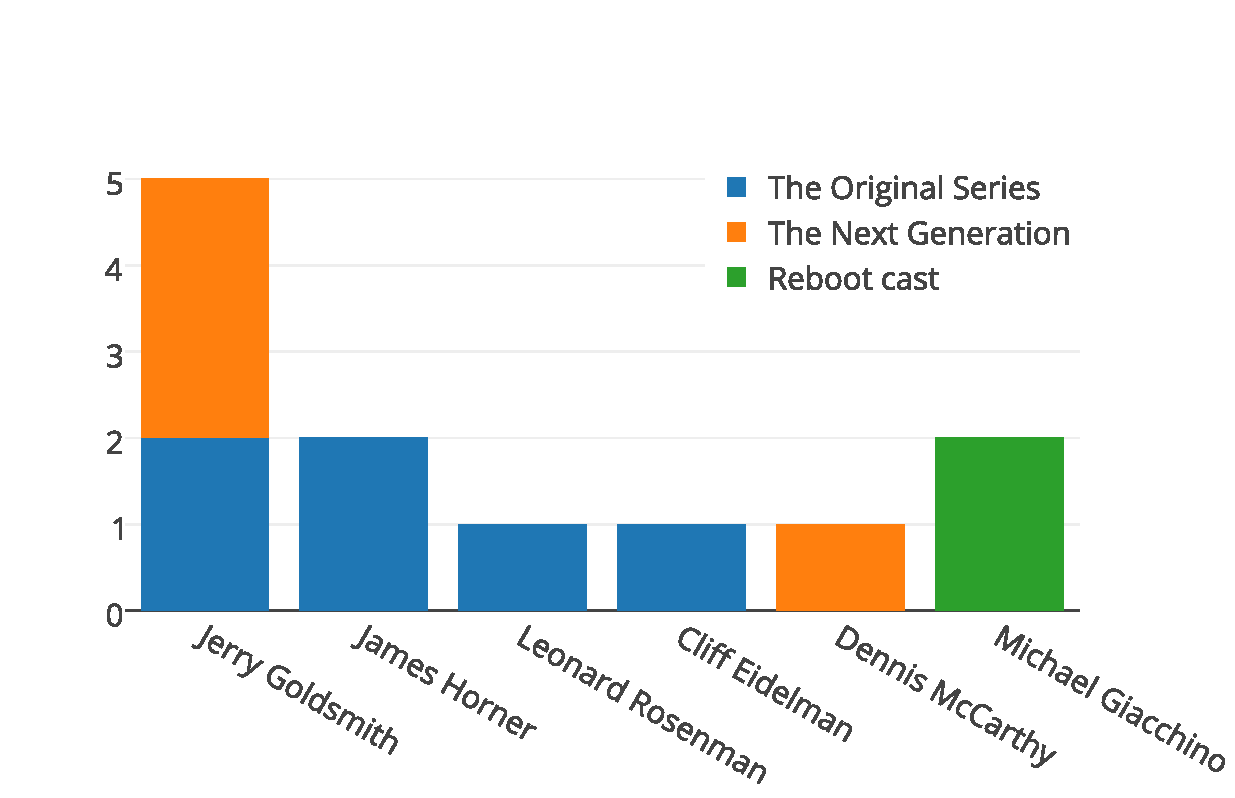
\includegraphics[width=\linewidth]{star_trek_composers_and_movies}
	\caption{Star Trek composers and movies}
	\label{fg:st composers}
	\setfloatalignment{b}
\end{figure}

But even so, there are no official scores to procure. I was able to get in touch with people able to help me get a look at the actual scores used during the different recording sessions, but that meant traveling to Hollywood and Paramount studios. By the time I had gotten this information any window to apply for funding was past. Therefore I chose to transcribe the music myself. One challenge of transcribing music this detailed is the amount of time required transcribing the examples. With twelve movies to chose from the question regarding what I was going to focus on arose. Star Trek, the movies is divided into three epochs: The Original Series, The Next Generation and the Reboot. I thought it best to choose two movies from each epoch. One composer in the Star Trek universe stands out: \textit{Jerry Goldsmith}. He has scored five of the twelve movies during a timespan of 23 year making him part of the quintessential \textit{sound} of Star Trek. The choice fell on the two first films, \textbf{''The Motion Picture''}, by Goldsmith and \textbf{''The Wrath of Kahn''}, by \textit{James Horner}. Both critically acclaimed for their music. The next obvious candidates was the newest films from the reboot series: \textbf{''Star Trek''} and \textbf{''Into Darkness''} featuring composer \textit{Michael Giacchino}. What to chose from ``The Next Generation'' era was harder. I wanted to study how the music has evolved over time therefore looking for some sort of continuity. The choice fell on Goldsmiths scores for \textbf{''First Contact''} and \textbf{''Nemesis''}. I present my analysis in chapter \ref{ch:sttmp} through \ref{ch:into_darkness}. That being said, the other scores are well worth the attention and should be included in a later research. A table containing the complete list of Star Trek movies can be found on page \pageref{tb:filmography} and the complete list of all composers associated with the Star Trek universe can be found on page \pageref{tb:star trek composers}.

\marginnote{
\textbf{The filmography in question:
}
\begin{itemize}
\item The Motion Picture, \textit{1979}, TOS 
\item The Wrath of Kahn, \textit{1982}, TOS 
\item First Contact, \textit{1996}, TNG 
\item Nemesis, \textit{2002}, TNG
\item Star Trek, \textit{2009}, Reboot 
\item Into Darkness, \textit{2013}, Reboot
\end{itemize}
}

Now my quest was crystalizing, I wanted to study the musical conventions of Star Trek. How to go about it? My formal training is for the most part traditional so the analytical tools I already knew was not ideal to handle the diverse tonality of movie scores. I knew ``Hollywoodian'' movie scores since \textit{Erich Wolfgang Korngold} and \textit{John Williams} had their roots in nineteen century classical music, also know as the romantic period of classical music. \textit{Romantic} music is mostly tonal, meaning it uses major and minor chords and scales to build the tonality, but it is not necessarily functional. By that I mean progressions build upon the \textit{circle of fifths} and the famous \(I-IV-V^{7}-I\). This brings us to the idea of a \textit{tonic}, a tonal ``home'' where we feel at peace after pursuing the chord furthest away from the tonic, the \textit{dominant}. It would be wrong to say that romantic music does not utilize the idea of a tonic, but it was not a concept expanded upon as they did in the classical era. Instead they had what I call \textit{tonal centers}. These are focal point for any given progression and stands as the root of origin. This differentiation is necessary because harmonic progressions can be made with a different logic than that of the circle of fifths. There are plenty of analytic tools to chose from when working with functional music and atonal music but I was having a hard time finding the right tool for non-unified tonal music.

During my research I came upon Frank Lehman's dissertation on \textit{''Reading Tonality Through Film: Transformational Hermeneutics and the Music of Hollywood'' (2012)}. His research was focusing on \textit{neo-Riemannian Theory}, a theory made to address the analytical challenges nineteen century music presented, applied to film music. I will discuss the application and execution of this theory in chapter \ref{ch:nrt}. To further explain how my analysis is constructed, I will discuss music analysis in general in chapter \ref{ch:musical analysis}. 

To aid the reader in analytic process I have chosen to include the transcriptions immediately following the corresponding analysis. The analytic legend will be discussed on page \pageref{fg:analysis legend} and finally I will present my conclusions in chapter \ref{ch:the musical conventions}.

As a final note I want to talk about what I am not covering in this thesis. First of all, I have chosen to use musical terms and notation to explain my findings. This means the reader will have to have a fairly advanced understanding of musical theory to fully appreciate the content of this thesis. I will not talk about film music history in general: How the film music traditions has evolved from live music to Korngold to Steiner to Williams and even Zimmer is extremely interesting, but it is covered to such an extent elsewhere there simply is no point including it and secondly, I do not believe being reminded of this knowledge will have an impact on the understanding of the main topic of this thesis. My goal is that the content of this thesis provides ample understanding of the main analysis and that the reader will come to appreciate the inner workings of the music in question and how it has evolved. 

% Revidert jan 2016
% !TEX encoding = UTF-8 Unicode
% !TEX root = ../../Masterthesis.tex

\chapter{Star Trek}\label{ch:star trek}

\begin{center}
\textit{Space: the final frontier. \\ These are the voyages of the starship Enterprise. Its continuing mission: \\ to explore strange new worlds, to seek out new life and new civilizations, \\ to boldly go where no one has gone before.}
\end{center}
\begin{flushright}
--- As narrated by Captain. Jean-Luc Picard \\
\parencite{day_boldly_2005}
\end{flushright}

%-----------------------------------------------------------------------------
% These Are The Voyages...
%-----------------------------------------------------------------------------

\section{These Are The Voyages...}

\begin{figure}
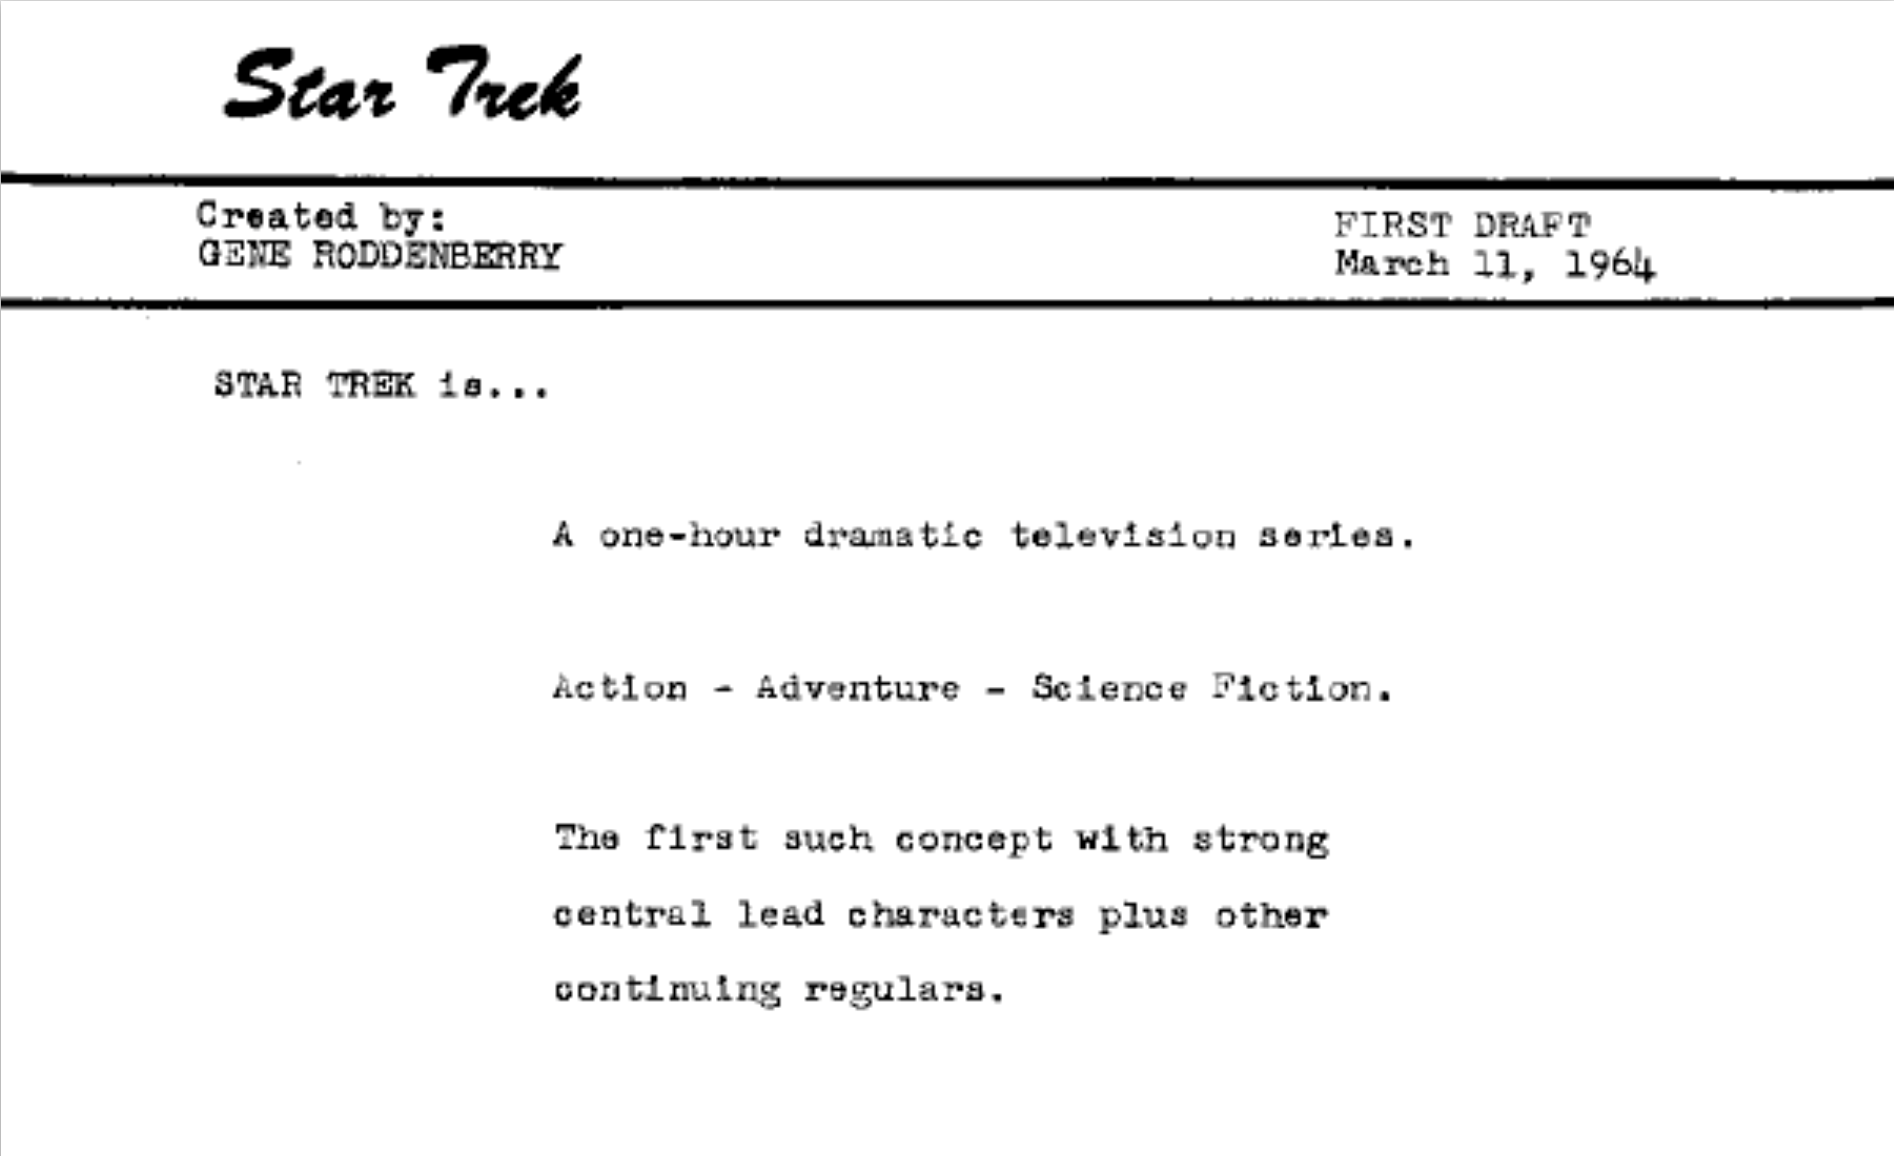
\includegraphics[width=\linewidth]{star_strek_roddenberry_pitch}
\caption{Gene Roddenberry's original pitch for Star Trek to NBC}
\end{figure}

\newthought{Star Trek is an} American science fiction TV and motion picture franchise, created by \textit{Gene Roddenberry}. It debuted with the pilot ``The Cage'' in 1966 on NBC and has since evolved into hundreds of books and novels, several computer games, six TV series\footnote{See table \ref{tb:tv series}}, and twelve motion pictures\footnote{See table \ref{tb:filmography}}. The basic premise of the show is an interstellar adventure in the beginning of the 23rd century where we follow the actions of the captains and crew on the starship Enterprise.\footnote{Except DS9 which takes place on a space station rather then a starship.} They follow the orders of \textit{Starfleet}, which is the scientific and exploratory branch of \textit{The United Federation of Planets}, a multi-planetary alliance. Star Trek displays a rather philanthropic view on the human race. The economy has moved away from capitalism, the crime rate is essentially zero. Religion is essentially obsolete. According to Roddenberry, humans in the 23rd century are,
\blockquote[{\cite{roddenberry_star_1987}}]
{
(...)intelligent, witty, thoughtful, compassionate, caring (...) -- but they have human faults and weaknesses too -- although not as many or as severe as in our time. (...)The major problems facing the human species have been resolved and the Earth has since been transformed into a human paradise.
}
The crew on the Enterprise consists of both humans and aliens, and the hierarchy and terminology used is in direct parallel with the Navy: they have ranks like Chief Petty Officer, Ensign, Captain, and Admiral and they use terms like ``port'' and ``starboard'' and the bridge is the main control room. 

\begin{margintable}
\small
\begin{tabular}{ll}
\toprule
	\textbf{TV-show}		& \textbf{Running}	\\
\midrule
    	The Original Series		& 1966-1969		\\
        The Animated Series		& 1973-1974		\\
        The Next Generation 	& 1987-1994		\\
        Deep Space Nine 		& 1993-1999		\\
        Voyager					& 1995-2001		\\
        Enterprise				& 2001-2005		\\
\bottomrule
\end{tabular}
	\caption{Star Trek TV series}
	\label{tb:tv series}
\end{margintable}

While Star Trek is widely regarded as a successful franchise, it had a rough start. \textit{The Original Series} ran for only three years. Even though the fan base was substantial, ever increasing budget cuts and tighter time schedules caused the show to finally call it quits in 1969. It would be 10 years before Paramount dared commit to a large scale motion picture. \parencite[87]{bond_music_1998}


%-----------------------------------------------------------------------------
% The Music of Star Trek
%-----------------------------------------------------------------------------

\begin{figure}
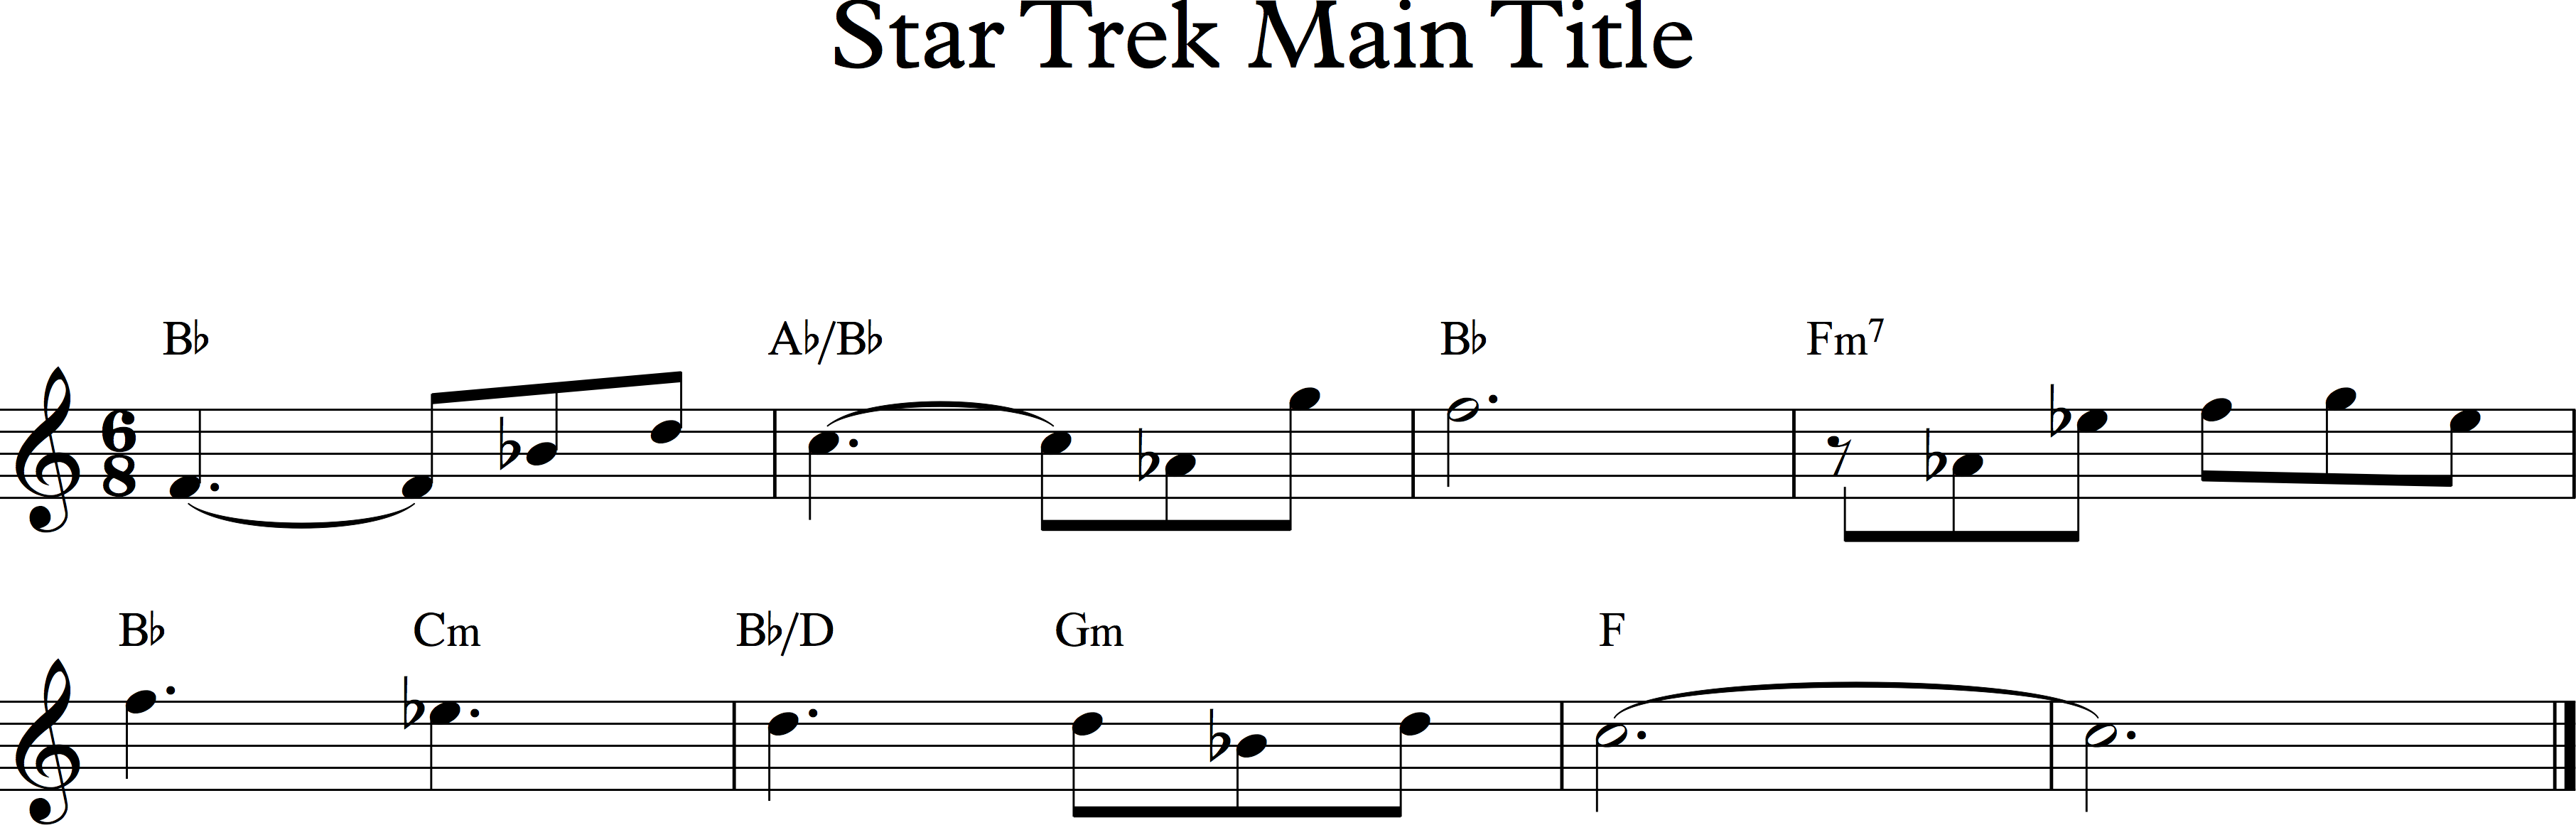
\includegraphics[width=\linewidth]{gfx/snippet_main_theme}
\caption{Goldsmith's ``Star Trek Theme''}
\end{figure}

\section{The Music of Star Trek} 

\marginnote{\textbf{Jerry Goldsmith} selected filmography: 
\begin{itemize}
\item Planet of the Apes (1968)
\item The Omen (1976)
\item Alien (1979)
\item Poltergeist (1982)
\item First Blood (1982)
\item Twilight Zone: The Movie (1983)
\item Total Recall (1990)
\item Basic Instinct (1992)
\item Mulan (1998)
\end{itemize}
}
Much like the Super Mario theme, the Star Trek theme is nearly ubiquitous in pop culture and is immediately recognized by most. In fact, Star Trek catch phrases have taken root in english vernacular. There are few that have not heard the phrase ``Beam me up, Scotty!'' or ``Damn it man. I'm a doctor, not a [\ldots]''. With similar influence, the music of Star Trek has pioneered what the ``future'' sounds like. The first Star Trek movie: \ac{ST:TMP}, directed by \textit{Robert Wise}, was planed as early as 1973, but Paramount did not have the confidence to finance an expensive and risky production. It was not until \textit{George Lucas}' space epic \textit{Star Wars (1977)}, scored by \textit{John Williams}, hit the theaters to enormous applause that Paramount gave \ac{ST:TMP} the green light \parencite{bond_music_1998}. \textit{The Original Series} had new music written for every episode, bearing the signature of some of the all time greatest composers in Hollywood\footnote{See table \ref{tb:star trek composers}}. However, when choosing who would compose the very first Star Trek motion picture, Paramount looked for a composer that could match the epic score of John Williams. \textit{Jerry Goldsmith (1929-2004)} had just finished the acclaimed 20th Century Fox production \textit{Alien (1979)} and had scored several science fiction blockbusters already, making him the perfect candidate \parencite[87]{bond_music_1998}. 

Much of the stylistic elements in \ac{ST:TMP} are borderline avant-garde and full of romantic elements. Goldsmith utilizes synthesizers, church organs, and a custom made instrument called ``Blaster Beam''.\footnote{
A musical instrument refined and made famous by Craig Huxley.
}
Some of the movie scenes are fairly long making some of the musical cues fairly long as well. Goldsmith utilizes this by building cues matching the slow tempo and thus bringing more traditional compositional couplings into the cue. In \nameref{sec:leaving drydock} (analyzed on p.~\pageref{sec:leaving drydock}) we see a cue 3:32 minutes long accompanying ``The drydock sequence''. Jeff Bond notes the following: \blockquote[{\cite[88]{bond_music_1998}}]
{
Maintaining interest in the scene was a task that mainly fell to Goldsmith, and the challenge resulted in a pice of music with an unusual amount of classical development and structure, a hallmark of Goldsmiths's epic style of the late `70s and early `80s.
}  
The now famous march Goldsmith composed later became the title track for the TV-series \textit{``The Next Generation''} making it what we could call the ``Star Trek Theme''.

\begin{table*}
\small
\begin{tabularx}{\linewidth}{p{5.2cm} p{3.2cm} l l}
		\multicolumn{4}{c}{Star Trek, movies and composers}\\
\toprule
		\textbf{Film} 					& \textbf{Composers}		& \textbf{Date Released}	& \textbf{Series}		\\
\midrule
		Star Trek: The Motion Picture		& Jerry Goldsmith			& 1979, 7 December 	& The Original Series 	\\
		ST II: The Wrath of Khan  			& James Horner				& 1982, 4 June  		& 					\\
		ST III: The Search for Spock  		& James Horner				& 1984, 1 June 			&  					\\
		ST IV: The Voyage Home				& Leonard Rosenman			& 1986, 26 November 	&  					\\
		ST V: The Final Frontier			& Jerry Goldsmith			& 1989, 9 June 			&  					\\
		ST VI: The Undiscovered Country		& Cliff Eidelman			& 1991, 6 December		&  					\\
		ST VII: Generations					& Dennis McCarthy			& 1994, 18 November		& The Next Generation	\\
		ST VIII: First Contact  			& Jerry Goldsmith\(\dagger\)& 1996, 22 November		&  					\\
		ST IX: Insurrection    				& Jerry Goldsmith			& 1998, 11 December		&  					\\
		ST X: Nemesis     					& Jerry Goldsmith			& 2002, 13 December		&  					\\
		Star Trek XI     					& Michael Giacchino			& 2009, 8 May			& Reboot Cast			\\
		ST XII: Into Darkness  				& Michael Giacchino			& 2013, 16 May			& 					\\
\bottomrule
    \(\dagger\) With his son Joel Goldsmith	&							&					&					\\
\end{tabularx}
    \caption{Star Trek filmography}
    \label{tb:filmography}
\end{table*}

\marginnote[2cm]{\textbf{James Horner} selected filmography: 
\begin{itemize}
\item Aliens (1986)
\item Honey, I Shrunk the Kids (1989)
\item Searching for Bobby Fischer (1993)
\item Braveheart (1995)
\item Apollo 13 (1995)
\item Titanic (1997)
\item Avatar (2009)
\item The Karate Kid (2010)
\end{itemize}}

\textbf{Star Trek II: The Wrath of Khan} was \textit{James Horner's (1953-2015)} big breakthrough as a feature film composer. The main reason Goldsmith was not utilized for this offering was budget cuts, making Horner -the ``new guy''- much cheaper to hire. Horner had scored a number of low-budget science fiction films previously, like \textit{``Humanoids From the Deep''} and \textit{''Battle Beyond the Stars''}, which incidentally has a striking similarity to the Star Trek II score.

The overall tone of the score owes much to Goldsmith and Williams; however, the score is manifestly Horneresque. The score is well loved by fans and critiques, despite the poor orchestral performance, which is under balanced and poorly executed.

Although not part of my thesis as such, it is worth noting some of the quite serious critique Horner has received for his compositional works. He is one of the most used composers in Hollywood but he has had to endure a lot of critique over the years for plagiarism. The case of artists ``borrowing'' from one another is not new and perhaps is impossible to avoid. The TED talk ``Embrace the Remix'' \footnote{\textcite{Ferguson2012}} discusses this phenomenon thoroughly. I believe no motif can be copyrighted as such, but they are part of a composers signature. In Horner's case the evidence would suggest that he not only borrows motives and harmonic progressions, but also references entire passages without giving credit to the original composer, like \textit{Sergei Prokofiev's - Alexander Nevsky: part 5}, which he references extensively in both his Star Trek scores, and Sergei Rachmaninov's theme from his first symphony. It is also very clear that he reuses his own material quite frequently, like the example mention earlier in which the similarity between \textit{``Battle Beyond the Stars''} main title and the main title of \textbf{Star Trek II} are quite striking.

\begin{marginfigure}
\center
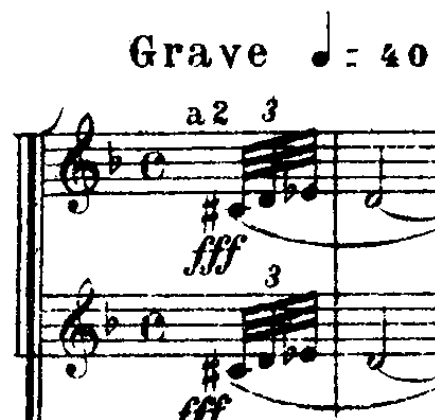
\includegraphics[width=0.7\linewidth]{rach_danger_motiv}
	\caption[Rachmaninov's 1st Symphony]{Snippet from the first bar of Rachmaninov's 1st Symphony. Exactly the same as Horner's ``Danger Theme'' which he has used throughout his career, and notedly in \textbf{Star Trek II}: ``Surprise Attack''}
	\label{fg:danger theme}
\end{marginfigure}

\textbf{Star Trek: First Contact} was directed by Star Trek actor \textit{Jonathan Frakes}, released in 1996 and was subject to high expectations because the previous \textbf{Star Trek: Generations} had been less of a success. While the overall looks of \textbf{Generations} was beautiful, the story had several weak points and distanced it self from the audience. The music got negative critique as well: \blockquote[{\cite[152]{bond_music_1998}}]
{MacCarthy's overture theme was memorable and his Nexus music quite beautiful, but the lack of repeated motifs and melodies in many of the other scenes lent a somewhat disconnected quality to the score as a whole.} 
The pressure was therefor on to remedy the damage done. Jerry Goldsmith was hired to do the job, but because of time pressure Goldsmith hired his son, \textit{Joel Goldsmith} to do the majority of action cues for the score. Joel produced total of 22 minutes of music for \textbf{First Contact}. 

\marginnote[-3cm]{\textbf{Michael Giacchino} selected filmography: 
\begin{itemize}
\item Medal of Honor: Underground (2000)
\item The Incredibles (2004)
\item Lost (2004)
\item Mission: Impossible III (2006)
\item Ratatouille (2007)
\item Up (2009)
\item Dawn of the Planet of the Apes (2014)
\end{itemize}}

\textbf{Star Trek: Nemesis} was the tenth, and last in the line of Star Trek films for some years to come. It was the third film featuring the cast of \textbf{The Next Generation} and was the mark of the end of an era. It was directed by \textit{Stuart Baird} and was released in 2002. Jerry Goldsmith was hired to score \textbf{Nemesis}, his fifth Star Trek movie (see figure \ref{fg:st composers}) and had long since become synonymous with the music of Star Trek \parencite{bond_2013}. Much of the score focuses on \textit{Shinzon's theme} (see figure \ref{shinzons_theme}), the main antagonist. Goldsmith treats his theme through several variations throughout the score\footnote{Hint's of it may be heard at the end of the main title \textit{Remus} and first heard clearly in the second half of \textit{Positronic Signal.}}. Goldsmith revisits themes from his past Star Trek movies in bits and pieces throughout, they are after all an important part of Star Trek lore, but he also created new themes that stand out as highlights of the movie. Like the new, heroic march in \textit{Battle Stations} \textquote[{\cite[215]{bond_2013}}]{(\ldots)that encapsulates Picard's sense of duty and his inherent nobility perfectly.}

\begin{marginfigure}
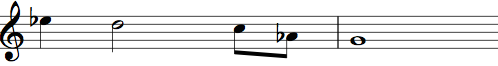
\includegraphics[width=\linewidth]{shinzons_theme}
	\caption{Part of Shinzon's Theme}
	\label{shinzons_theme}
\end{marginfigure}

In 2009 \textbf{Star Trek}, directed by \textit{J.J. Abrams}, came to cinemas across the world. Michael Giacchino, a regular collaborator of Abrams', was to pick up the mantle after Goldsmith. With almost 30 years of Star Trek history, expectations for Giacchino's score was high. The score turned out to strike out in a new branch leaving the old thematic material behind for a new, omnipresent theme Giacchino uses in virtually every major cue. All over, Giacchino's score use a simpler harmonic language, and lacks the ``sci-fi adventure'' found in Goldsmith and Horner's Star Trek scores. \textbf{Star Trek} did suffer from post production difficulties regarding the sound FX and music. The music got reworked extensively on the cutting floor, making analyzing the music from the source harder, due to the layers of dialogue and special-effects.
\footnote{
\textquote[\cite{takis_score_2010}]{In some cases, cues that had been displaced from their intended positions were replaced or supplemented by editorial creations.}
}
Fortunately a ``Deluxe'' edition CD was released which figured many of the original, unaltered cues. This, combined with the altered cues we hear in the movie score, gives us a reasonable view of the overall sonority.

\textbf{Star Trek: Into Darkness} is the second of the rebooted series, and was released in 2013 with J.J. Abrams and Giacchino at the helm. Now a defined part of something new, the sweeping romantic grandeur from Goldsmith's time is part of the \textit{Ars Antiqua}. Apart from the overall flattened harmonic complexity the score suffers from a low and lifeless mix in the final movie. Nevertheless, the score is more intricate than the 2009 movie and shows that Giacchino now had the time to evolve the sound and adapt it to the new universe. 

\begin{table*}
\small
\begin{tabularx}{\linewidth}{lllX}
\toprule
	\textbf{Composer}	& \textbf{Movie score} 				& \textbf{Series theme} 			& \textbf{Incidental music} \\
\midrule
	Alexander Courage 	& 								& The Original Series 			& The Original Series \\
	Cliff Eidelman 		& ST VI: The Undiscovered Country 		&  							&  \\     
	David Bell			&  								&  							& Deep Space Nine, Voyager, Enterprise \\ 
	Dennis McCarthy 	& ST VII Generations 				& Deep Space Nine 				& The Next Generation, Deep Space Nine, Voyager, Enterprise \\
	Diane Warren 		&  								& Enterprise 					&  \\    
	Fred Steiner 		&  								&  							& The Original Series, The Next Generation \\     
	George Duning 	&  								&  							& The Original Series \\     
	Gerald Fried 		& 								&  							& The Original Series \\     
	James Horner 		& ST II: The Wrath of Khan			&  							&  \\   
					& ST III: The Search for Spock 			&  							&  \\     
	Jay Chattaway 		&  								& 							& The Next Generation, Deep Space Nine, Voyager, Enterprise  \\    
	Jerry Goldsmith 	& ST: The Motion Picture				& The Next Generation   			&  \\     
					& ST V: The Final Frontier				& Voyager						&  \\     
					& ST VIII: First Contact				& 		 					&  \\     
					& ST: IX Insurrection					&  							&  \\     
					& ST X: Nemesis 					&  							&  \\     
	Leonard Rosenman 	& ST IV: The Voyage Home 			&  							&  \\     
	Michael Giacchino 	& Star Trek XI						&							&  \\
					& ST XII: into Darkness 				&  							&  \\     
	Paul Baillargeon 	&  								& 							& Deep Space Nine, Voyager, Enterprise \\ 
	Ron Jones 		&  								&  							& The Next Generation \\ 
	Sol Kaplan 		&  								&  							& The Original Series \\ 
	Velton Ray Bunch 	&  								&  							& Enterprise \\     
\bottomrule
\end{tabularx}
\caption{List of Star Trek composers}
\label{tb:star trek composers}
\end{table*}

% Reviewd jan 2016

% !TEX encoding = UTF-8 Unicode
% !TEX root = ../../Masterthesis.tex

\chapter{Musical analysis}\label{ch:musical analysis}

\newthought{The analysis portion} of this thesis is organized into cues chronologically. Each subject cue is treated in two parts. The first part contains the primary analytical body. Following is the transcription, which ranges from a plain harmonic analysis to full-on orchestral transcriptions. The reason they are located here, and not in the end as an appendix, is because it will be handy to refer to them while reading through the analysis.

My analysis will cover several angles of approach. Mostly I will be looking at harmonic patterns, i.e. the relationship and logic between harmonic transformations, but I will comment on tonality and sonority produced by melodies and/or orchestration. Although the main body of this understanding stems from Frank Lehman's work on \acf{nRT} applied to film music, traditional analysis is very much part of the total picture. However, as I will try do describe throughout chapter \ref{ch:nrt}, the traditional way of explaining tonal progressions in relation to a traditional tonic in regard to film music is forfeit.

\begin{marginfigure}[-6cm]
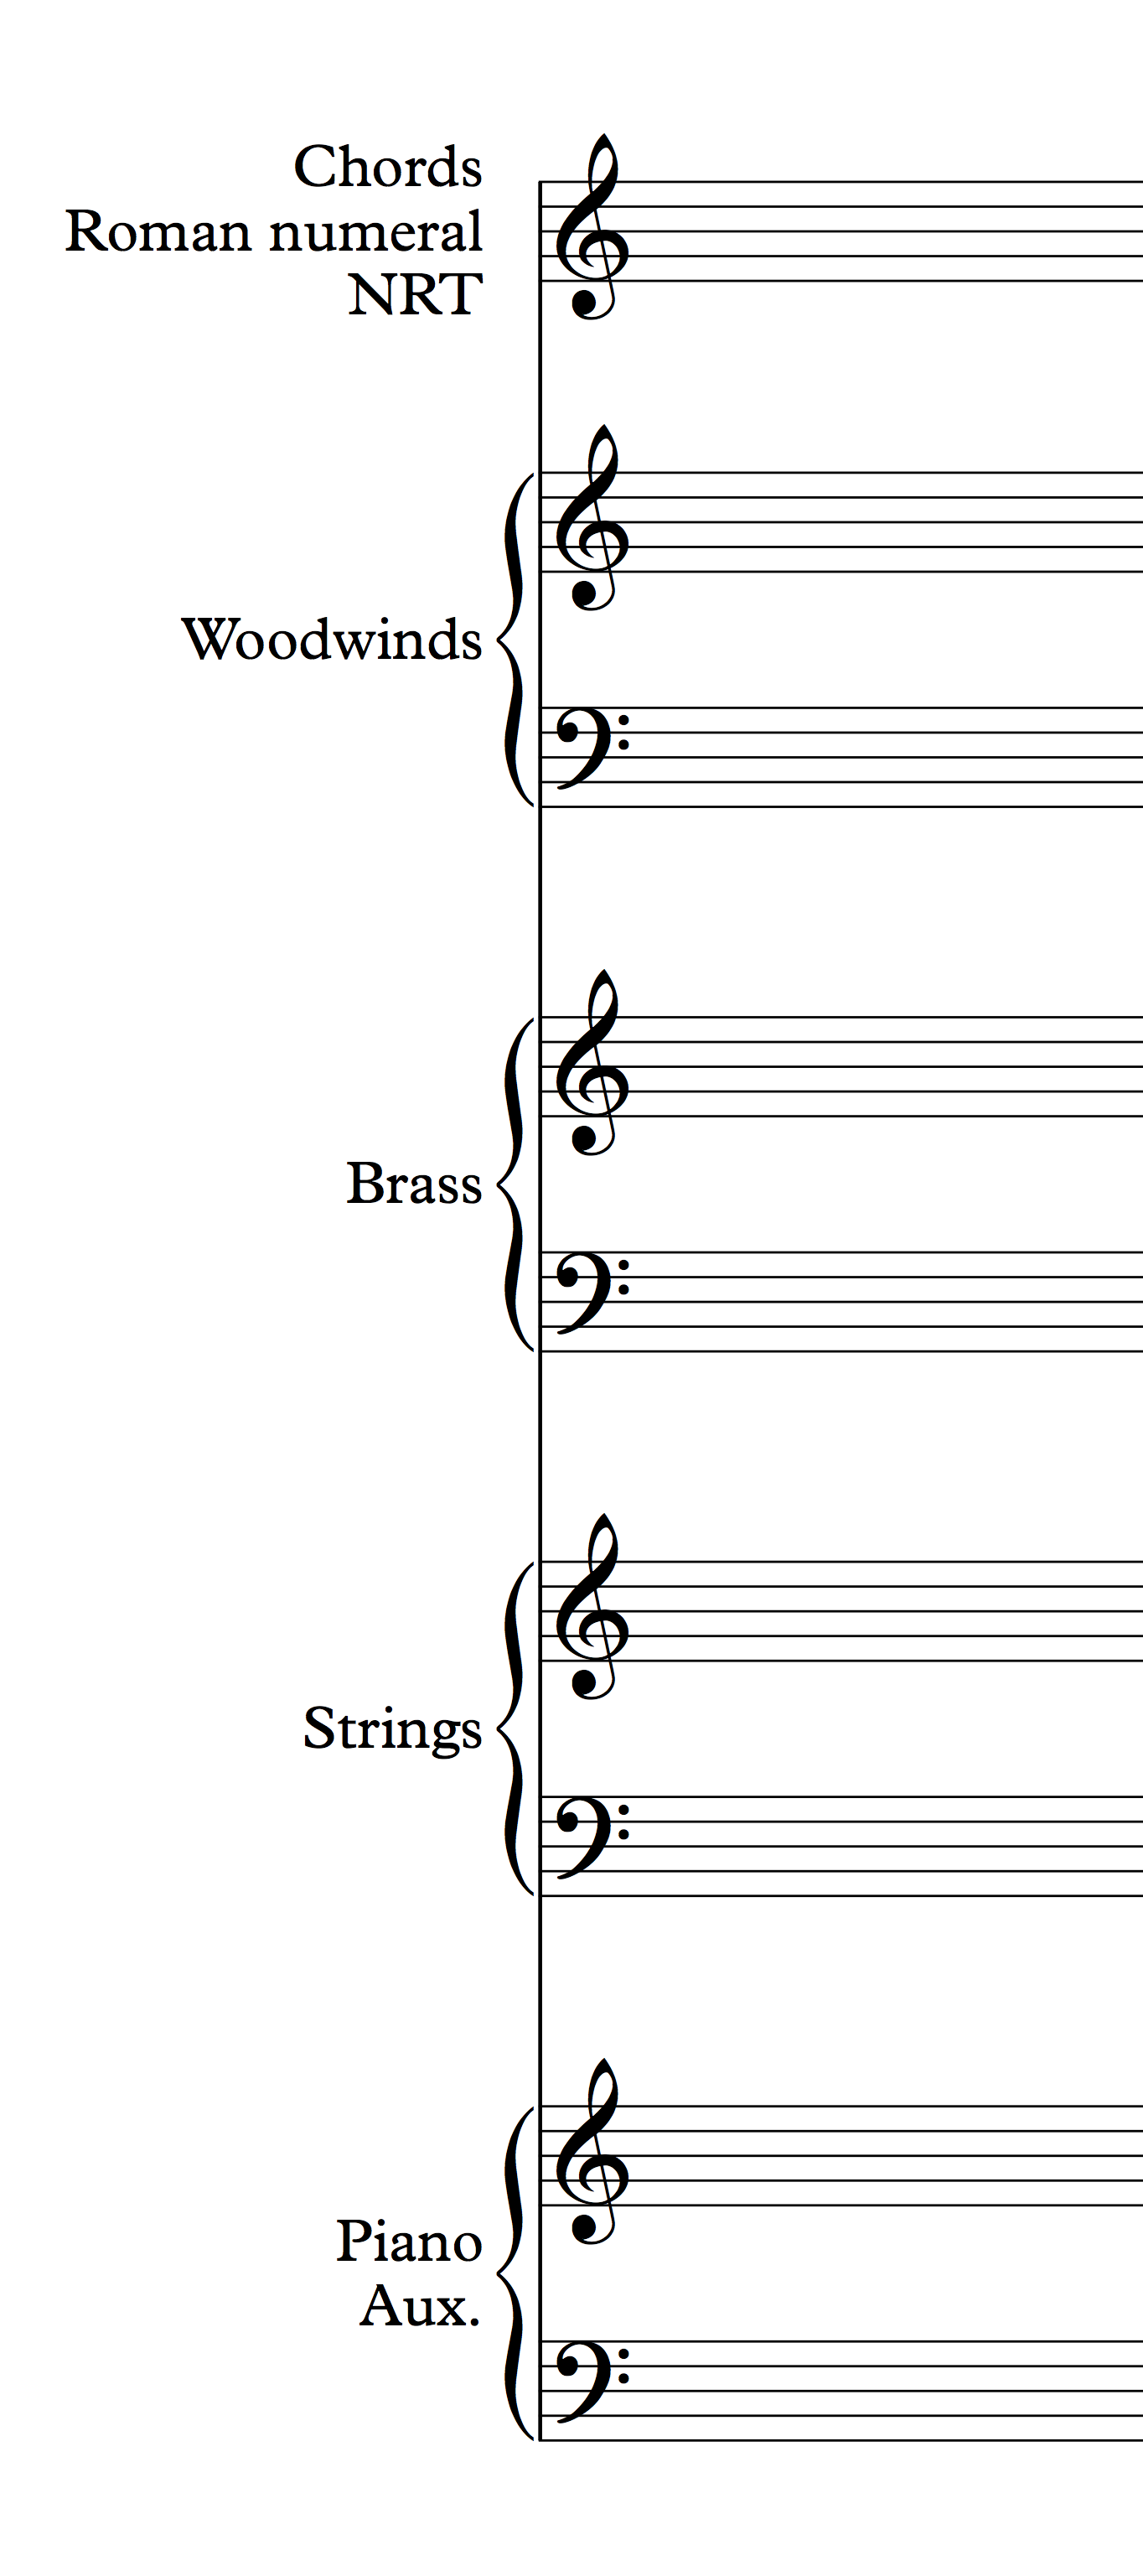
\includegraphics[width=\textwidth]{analysis_legend}
	\caption{Analysis Legend}
	\label{fg:analysis legend}
\end{marginfigure}

\begin{marginfigure}
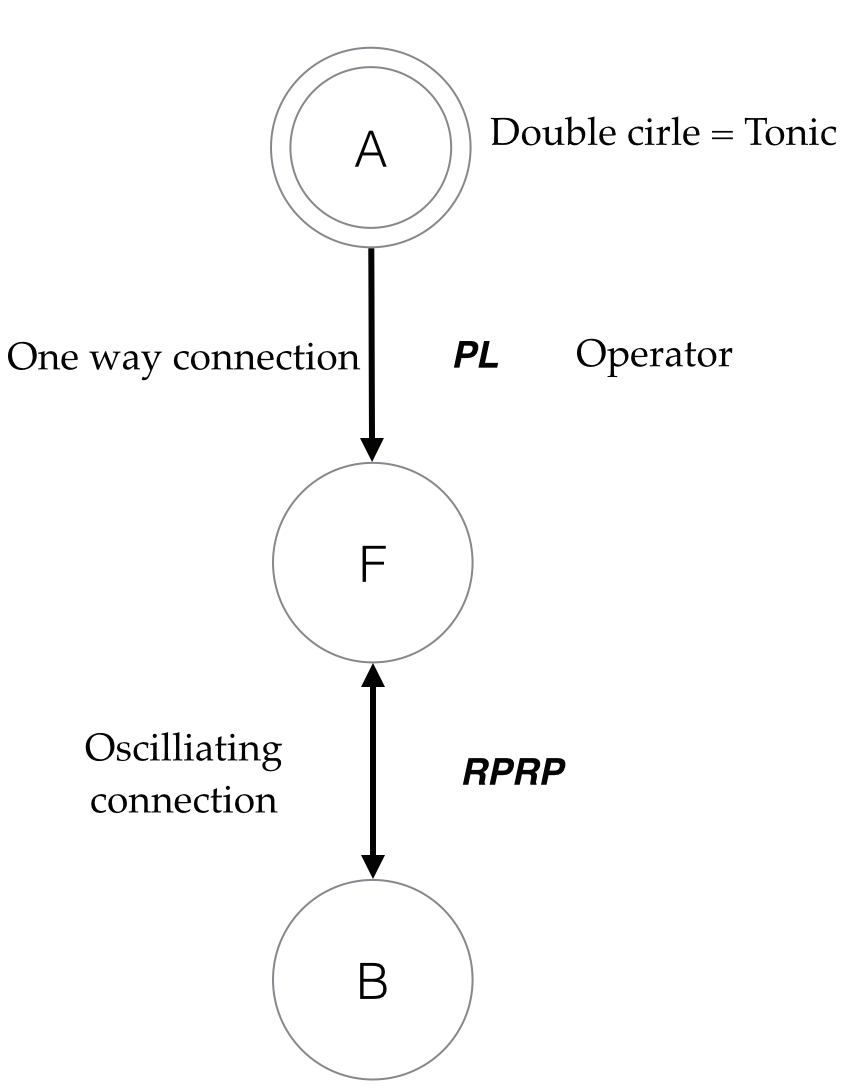
\includegraphics[width=\linewidth]{NRT_legend}
	\caption{nRT analysis legend}
	\label{fb:nrt legend}
\end{marginfigure}


In this chapter I will explain how I intend to use traditional tools. My musical background is from two very different worlds: One side of my training is classical orchestration and composition, and the other is that of a professional musician, primarily playing non-classical literature like jazz, fusion, and progressive rock. While reading academic papers on music theory, I have come across some quite creative ways to notate chords as unambiguously as possible. For the most part they feel un-intuitive for me as a musician. My solution is to alternate chord notation in two ways, both standardized in the performing world of musicians. The first and primary way is based on jazz traditions, C for C major, Cm for C minor and superscripts for added non-triadic pitches, like \chord{C}{maj7}. Superscripted integers assumes the diatonic scale except chords considered dominant, i.e. \chord{C}{7},\chord{C}{9}, \chord{C}{11} and \chord{C}{13}. Superscripted integers in parenthesis assume an alteration of that specific scale degree. The second way is to supply \textit{Schenkerian} roman numerals, using superscripts for added non-triadic pitches wherever possible or practical. I will try to use roman numerals to show scale degree but sometimes it simply is not ideal because film music is governed by what is happening on the screen, not by classical conventions. Or as Lehman puts it: \textquote[{\cite[180]{Lehman_2013}}]{It is defiantly “non-absolute” music, composed as but one part of a superordinate text.}. Thus, since film music seldom is rooted in a specific key I will refrain from giving key signatures unless very clear indications of the opposite. When practical I will draw Schenker graphs to illustrate a underlying harmonic pattern. I will indicate possible keys below the staff. \textit{Inversions} containing pitches in the root triad will be handled using the letters \(_{b, c}\) or \(_{d}\) - the latter used for hexachords and/or diminished chords. Non-triadic pitches will be displayed with a /, like C/B\(\flatx\). When sheet music is impractical, I'll refer to pitches by name or \textit{pitch classes}, (\textit{pc}), using brackets [~] and sometimes a keyboard illustration\marginnote[-2cm]{\keyboard{C,D,E,F,G,A,Bess,B}}. Unless otherwise noted, \textit{pitch class} assumes an absolute 0 regardless of key signature, making 0=C and 11=B. Step 10 and 11 are usually referred to as t and e. It is important to note that I will transpose every example given by pitch classes to C. When I need to talk about specific \textit{scale degree} in relation to a chord, I'll use a \textit{caret} to indicate this. Ex.: The \(\hat{3}\) of C=E.

% !TEX encoding = UTF-8 Unicode
% !TEX root = ../../Masterthesis.tex

\chapter{neo-Riemannian Theory}\label{ch:nrt}
% \morefloats

\newthought{Traditional} tonal harmonic analysis is designed to handle the sonorities constitutionalized in the Baroque and Classical eras. The idea is that any given chord tells something about where it stands in relation to the chord preceding it. Put rather bluntly every chord, given a long enough chain, could be interpreted as a dominant or a part of a cadence heading for, or avoiding a tonic. While this is perfectly adequate for most diatonic-based music, chromatic music that is triadic but not altogether unified under a diatonic rule, does serve a challenge for traditional functional analysis. \acf{nRT}\footnote{The abbreviation is nRT, with a small \textit{n} pointing to the fact that this maybe has grown beyond the \textit{''neo''} tag. \textquote[{\cite[1]{Lehman_2015}}]{(...)this no-longer so ``neo'' theoretical system.}} was developed to handle this issue.

Let us examine the following:

\begin{figure*}[h!]
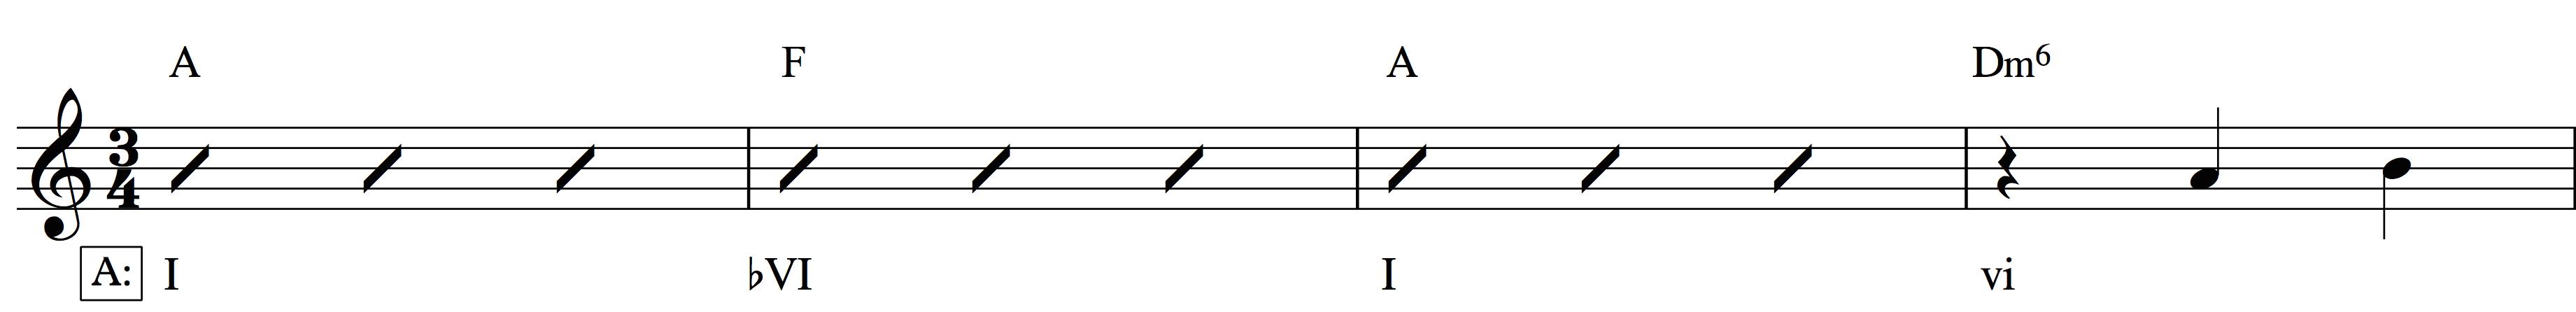
\includegraphics[width=\linewidth]{Ilia_Theme_1}
	\caption{Ilia's Theme 1}
	\label{Ilia_Theme_1}
	%\setfloatalignment{b}
\end{figure*}

\begin{figure}[h!]
\center
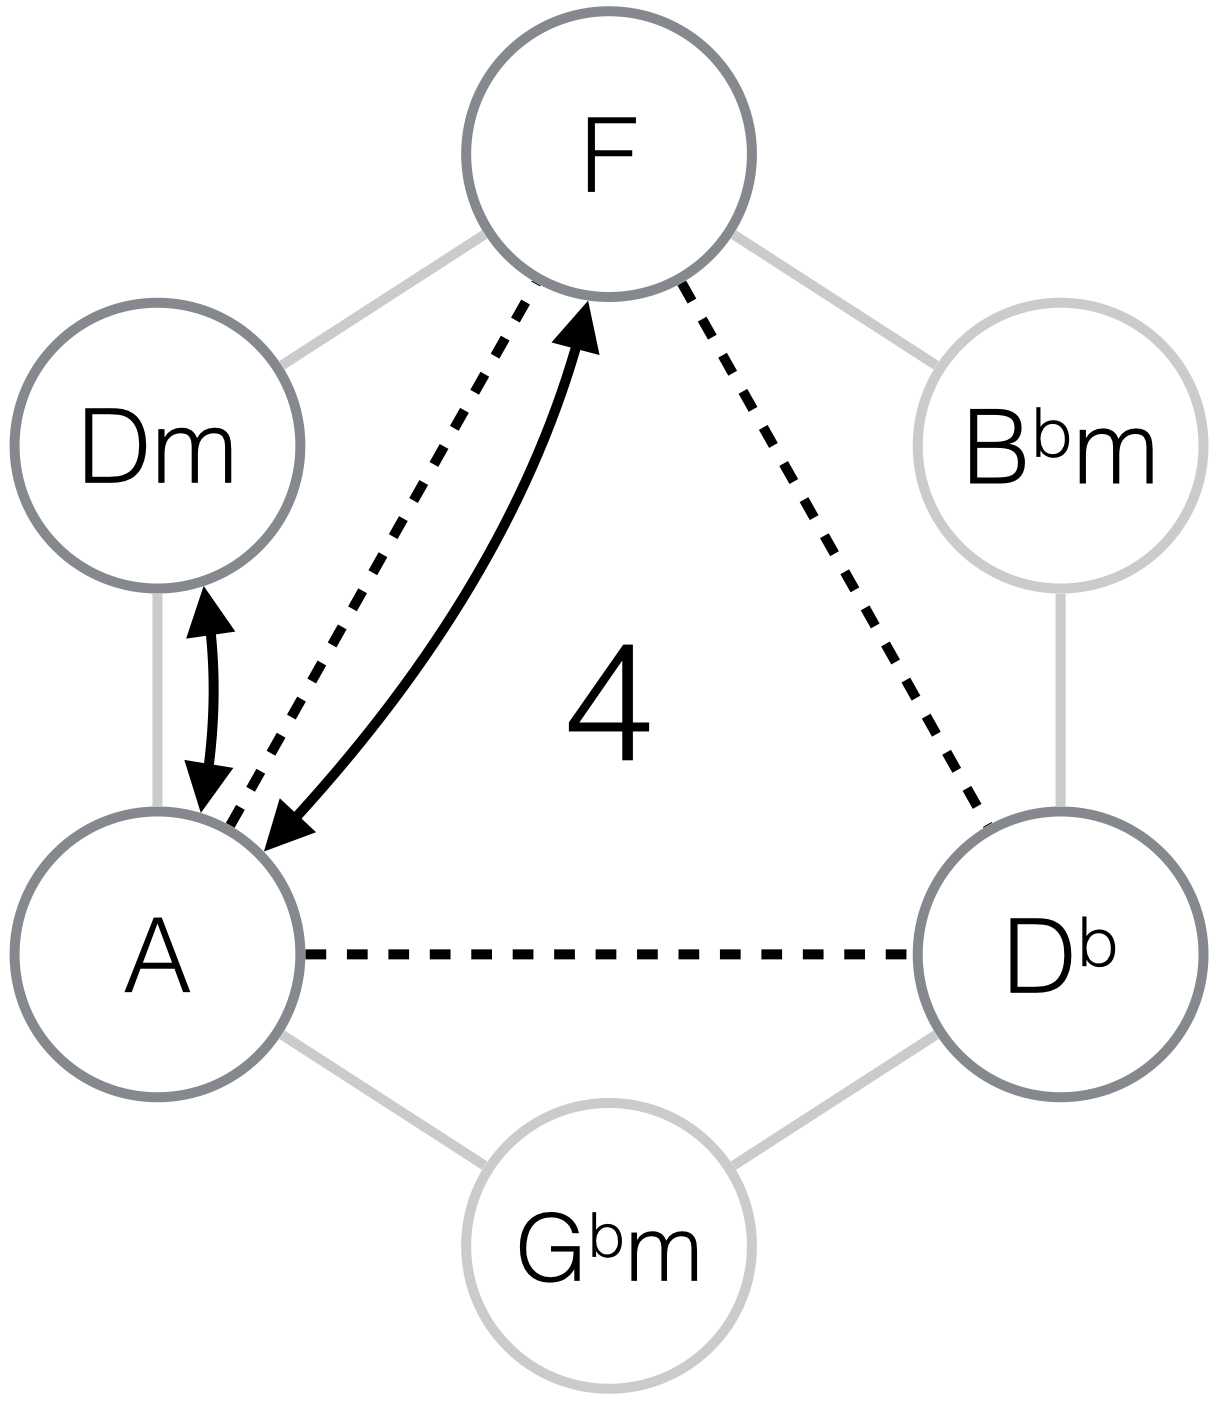
\includegraphics[width=0.5\linewidth]{Ilia_theme_1_nrt}
	\caption{Ilia's Theme m. 1-4}
	\label{Ilia_theme_1_nrt}
	\setfloatalignment{b}
\end{figure}

\noindent This show an excerpt from Goldsmith ``Ilia's Theme'' from \ac{ST:TMP}\footnote{See the complete sheet music on page \pageref{Ilias_Theme}}. If one where to analyze this using traditional tools we immediately run into a problem: What to define as the tonic? If we assume A, then F becomes \(\flatx{VI}\), and this makes sense because the \chord{Dm}{6} makes what we can identify as a \textit{Hollywood Cadence} \(({iv}\Rightarrow{I})\). If we assume F, then A becomes \(III\) and the \chord{Dm}{6} becomes \(vi\) which also makes sense. Within the context of a circle of fifths it makes no sense at all as it fits neither heads or tail of the Tonic, Subdominant, Dominant triangle for neither A nor F. So right from the get-go we have two possible candidates for a tonic. The same dichotomy of tonality continues throughout the first part of the cue.

\begin{figure*}[h!]
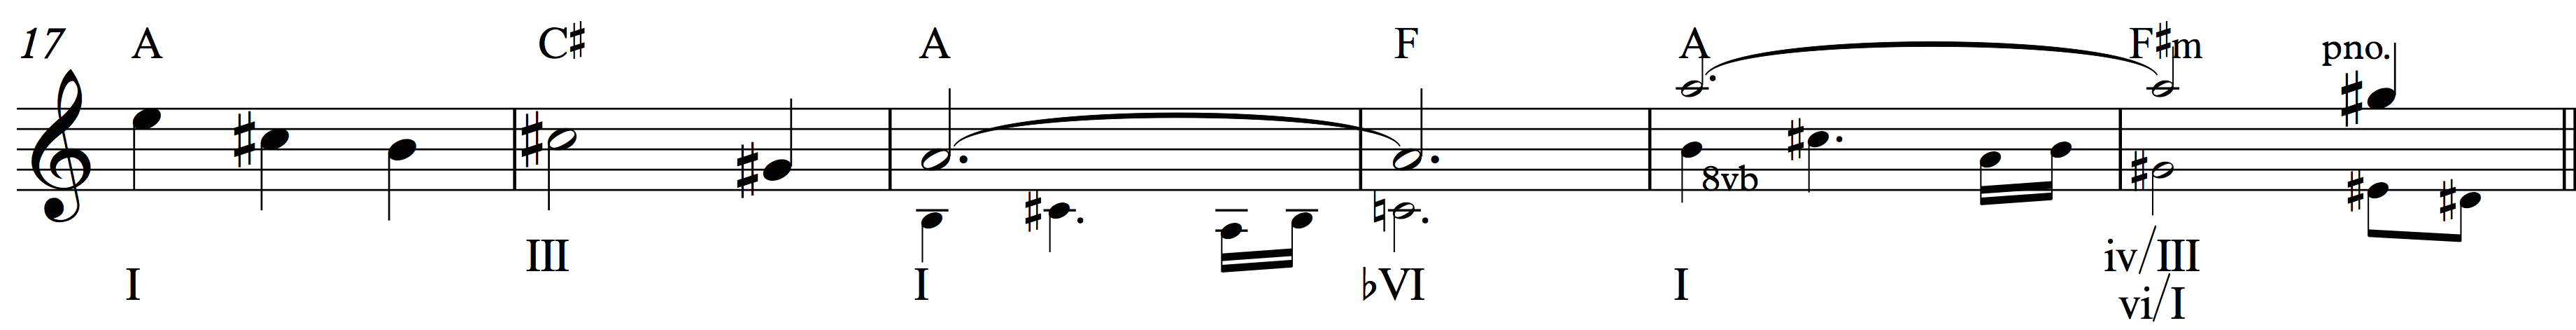
\includegraphics[width=\linewidth]{Ilia_Theme_2}
	\caption{Ilia's Theme 2}
	\label{Ilia_Theme_2}
	\setfloatalignment{b}
\end{figure*}

In \textbf{m.17-22}, figure \ref{Ilia_Theme_2}, we see some movement that further could indicate A as tonic seeing that we have both \(III/A\) and \(vi/A\), acting internally as \(V/vi-i/vi\) and prepare us for \textbf{m.23} where the yet another juxtaposition seems to unfold: figure \ref{Ilia_Theme_3}.

\begin{figure*}[h!]
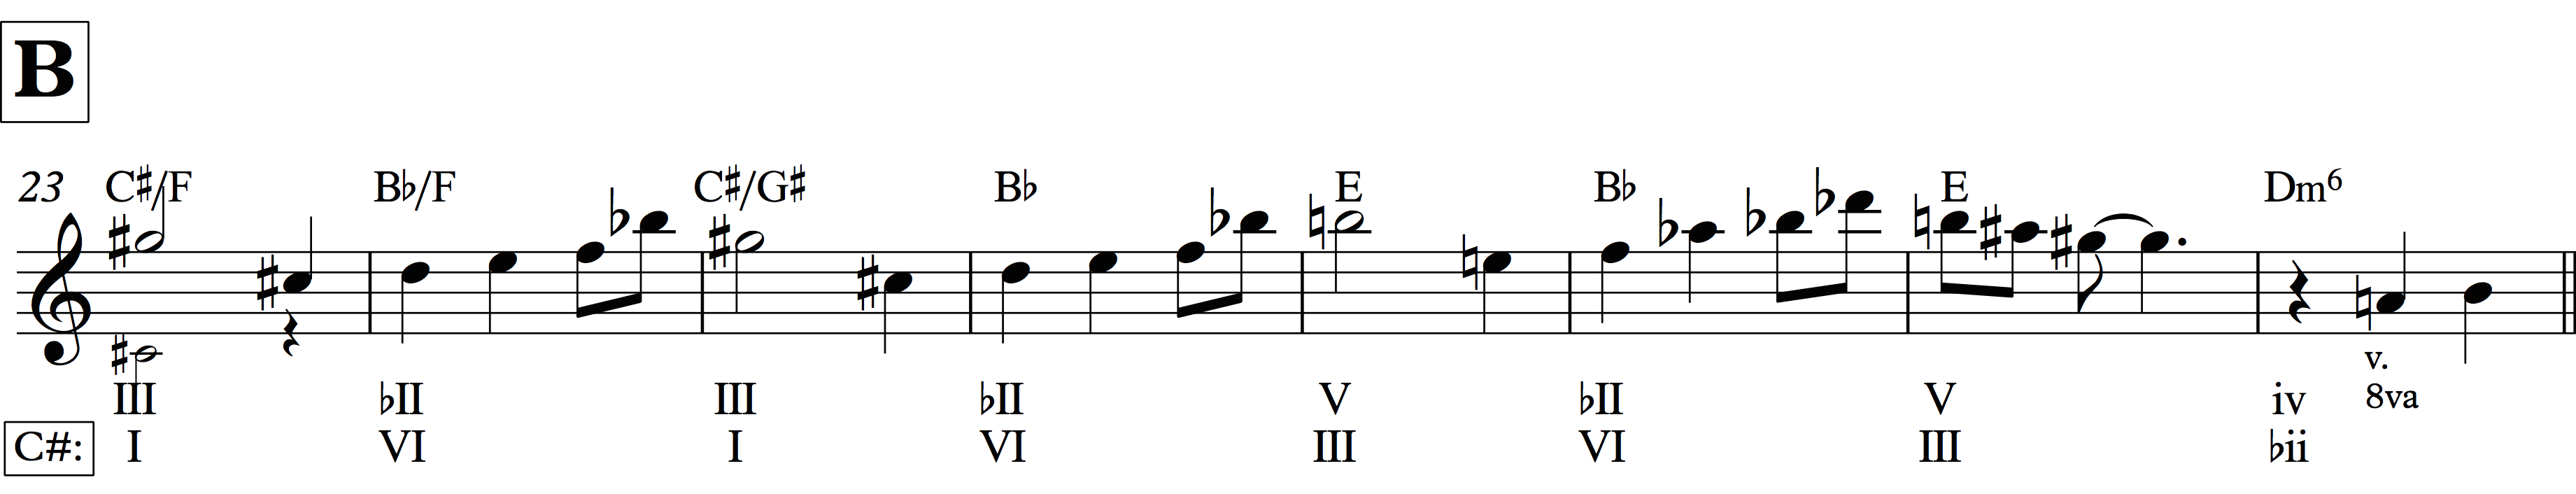
\includegraphics[width=\linewidth]{Ilia_Theme_3}
	\caption{Ilia's Theme 3}
	\label{Ilia_Theme_3}
	%\setfloatalignment{b}
\end{figure*}

Now \dflat/\ciss revolves around \bflat and then \bflat and E before ending on \chord{Dm}{6}. The internal logic does not comply with the ordinary predictions we can make from \(I-IV-V\) and its children. If we, however, apply the logic from transformational analysis we get to another picture. 

We can make a circle of chords based on different transformations then that of the circle of fifths, in this case major thirds, we can see some sort of logic underpinning the progression. If we assume A as the \textit{tonal centre} we can see that by moving from \(I\) to \(iv\) making it the new \(vi\) we get the formula: \({I}\Rightarrow{iv/vi}\) thus producing a circle of thirds. This circle is know as a \textbf{NR\(_{4}\)} circle and I will explain these circles in greater detail further down the chapter. With this we have a model that explains the majority of the first part. 

\begin{figure}[h!]
\center
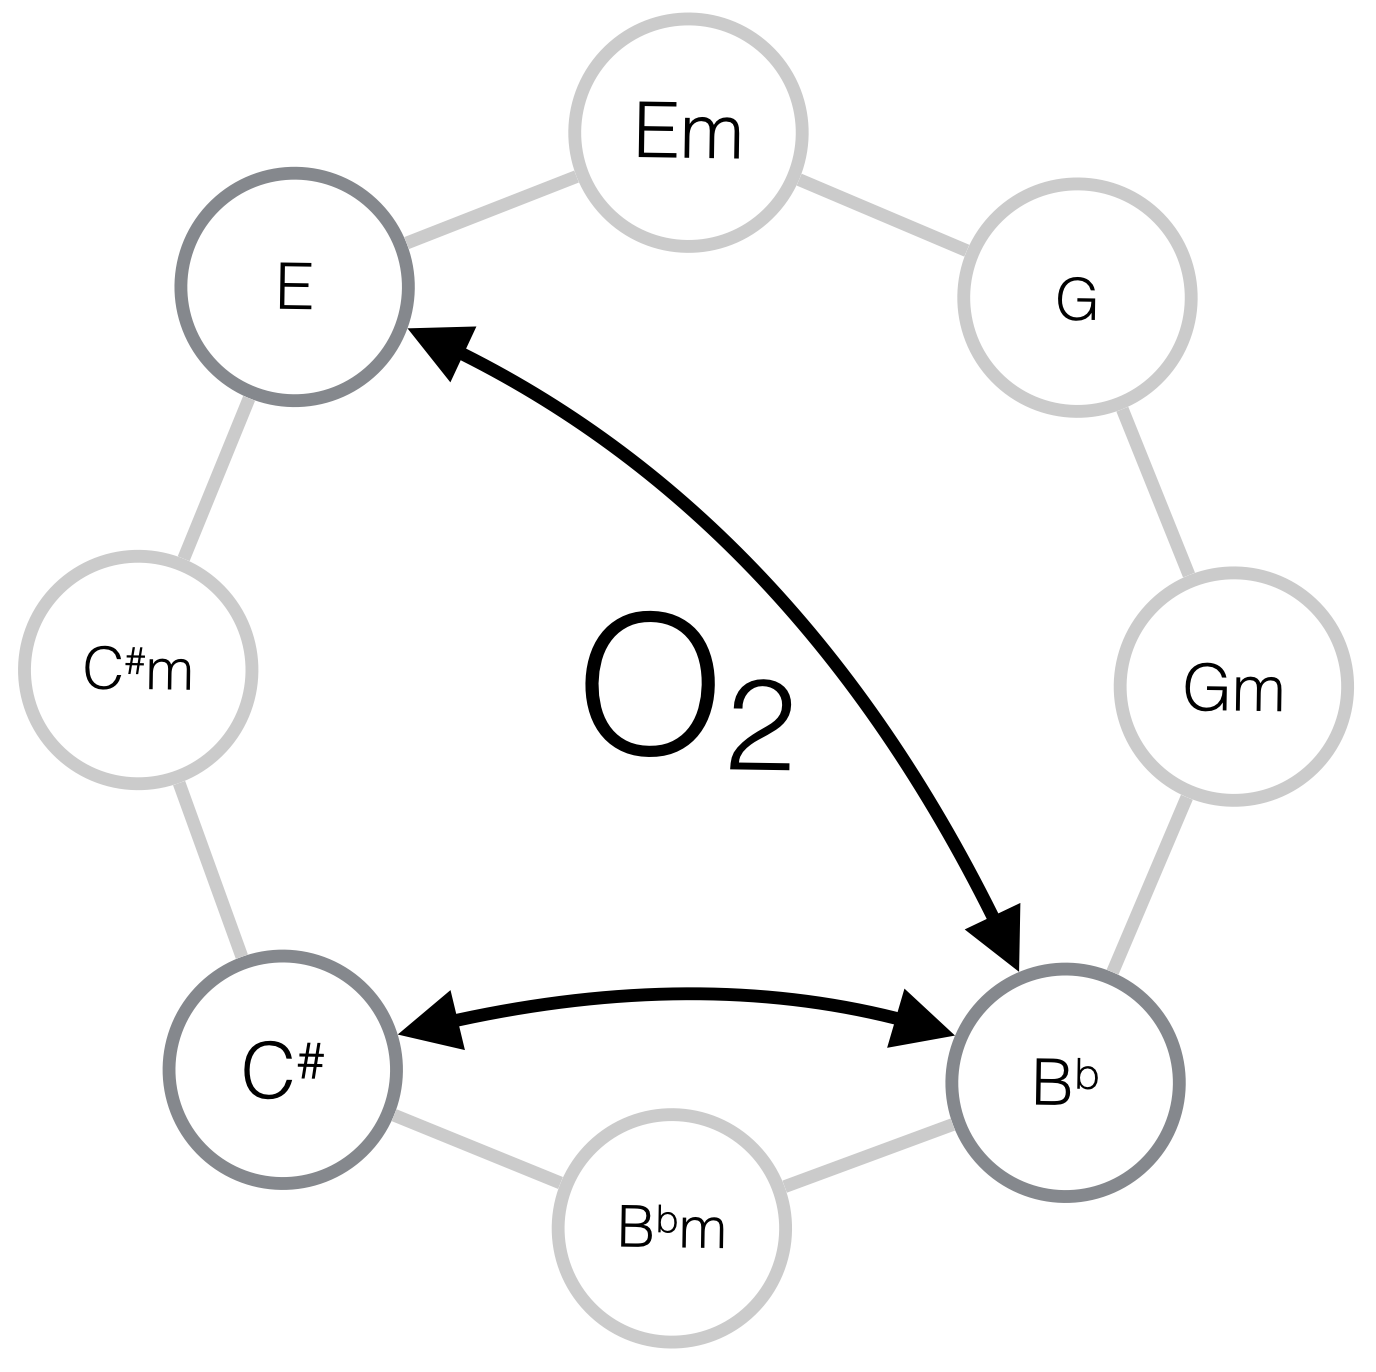
\includegraphics[width=0.55\linewidth]{Ilia_theme_2_nrt}
	\caption{Ilia's Theme, m.23-29}
	\label{Ilia_theme_2_nrt}
	\setfloatalignment{b}
\end{figure}

With the second part, figure \ref{Ilia_Theme_3}, we can build a figure, (\ref{Ilia_theme_2_nrt}) using the same logic; a \textit{hexatonic} circle of thirds that we can see is in relation with the movements in \textbf{m.23-30} where the tonal centre is \ciss from which it is possible to build a \textit{octatonic} circle of minor thirds, and thus making the relationship between \bflat and E not so far fetched as one might think. To top it of, one might make a compound diagram that shows that the two parts are indeed related thanks to the common chord \ciss. The conclusion from this short example is that the chord structure is largely govern by thirds and that \textbf{m.1-22} (Letter A) and B has a common root.

\begin{figure}[h!]
\center
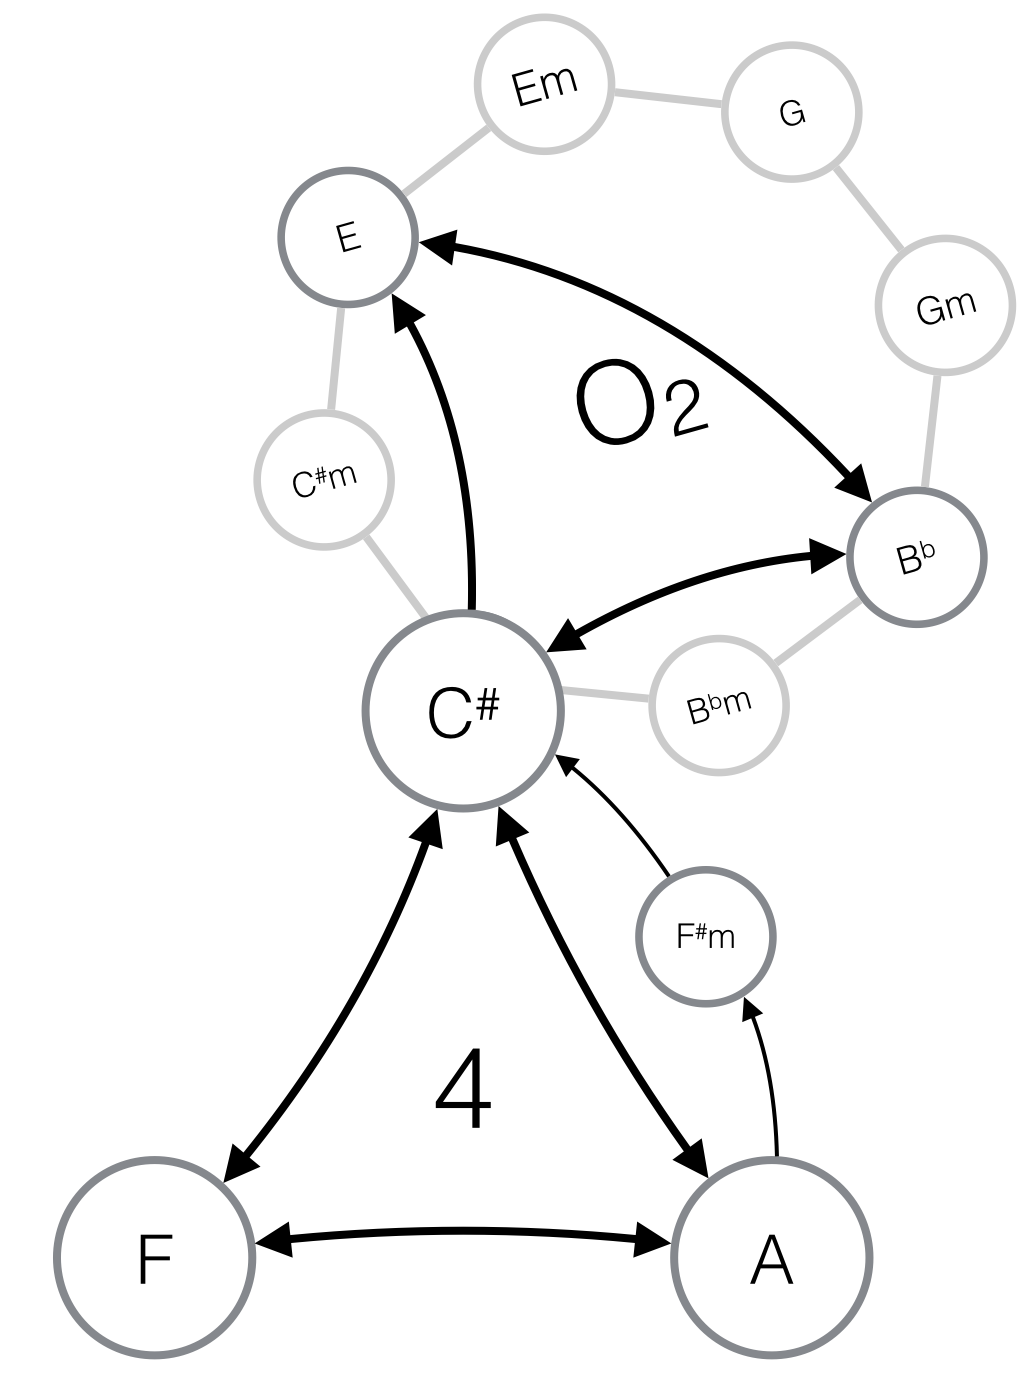
\includegraphics[width=0.55\linewidth]{Ilia_theme_3_nrt}
	\caption{Ilia's Theme, m.17-29}
	\label{Ilia_theme_3_nrt}
	%\setfloatalignment{b}
\end{figure}

\ac{nRT} originates from David Lewin. He wrote an essay in 1987 titled: \textit{``Generalized Musical Intervals and Transformations''}\footnote{\textcite{lewin_generalized_2007}. I suggest reading Richard Cohn's introduction to neo-Riemannian theory, \parencite{cohn_introduction_1998} for those of historically inclined as I will not cover the historical backdrop in this thesis.} that laid the premise for this type of transformational analysis. According to Cohn it was created to serve the analytical needs of nineteenth century music. Film music tonality has a lot of commonality with nineteenth century tonality in that the tonality is mostly tonal, but ununified\footnote{\textcite[p.2]{cohn_introduction_1998}}, i.e. not bound by a diatonic scale. Since Lewin's essay where published, the theory has gained traction with the likes of Richard Cohn\footnote{\textcite{cohn_maximally_1996}} and Frank Lehman\footnote{\textcite{lehman_reading_2012}}, among others. Lehman's work on how to apply \textit{transformational analysis}, as this branch of theory is called, to film music is what has enabled me to do this thesis.

\begin{figure*}
\center
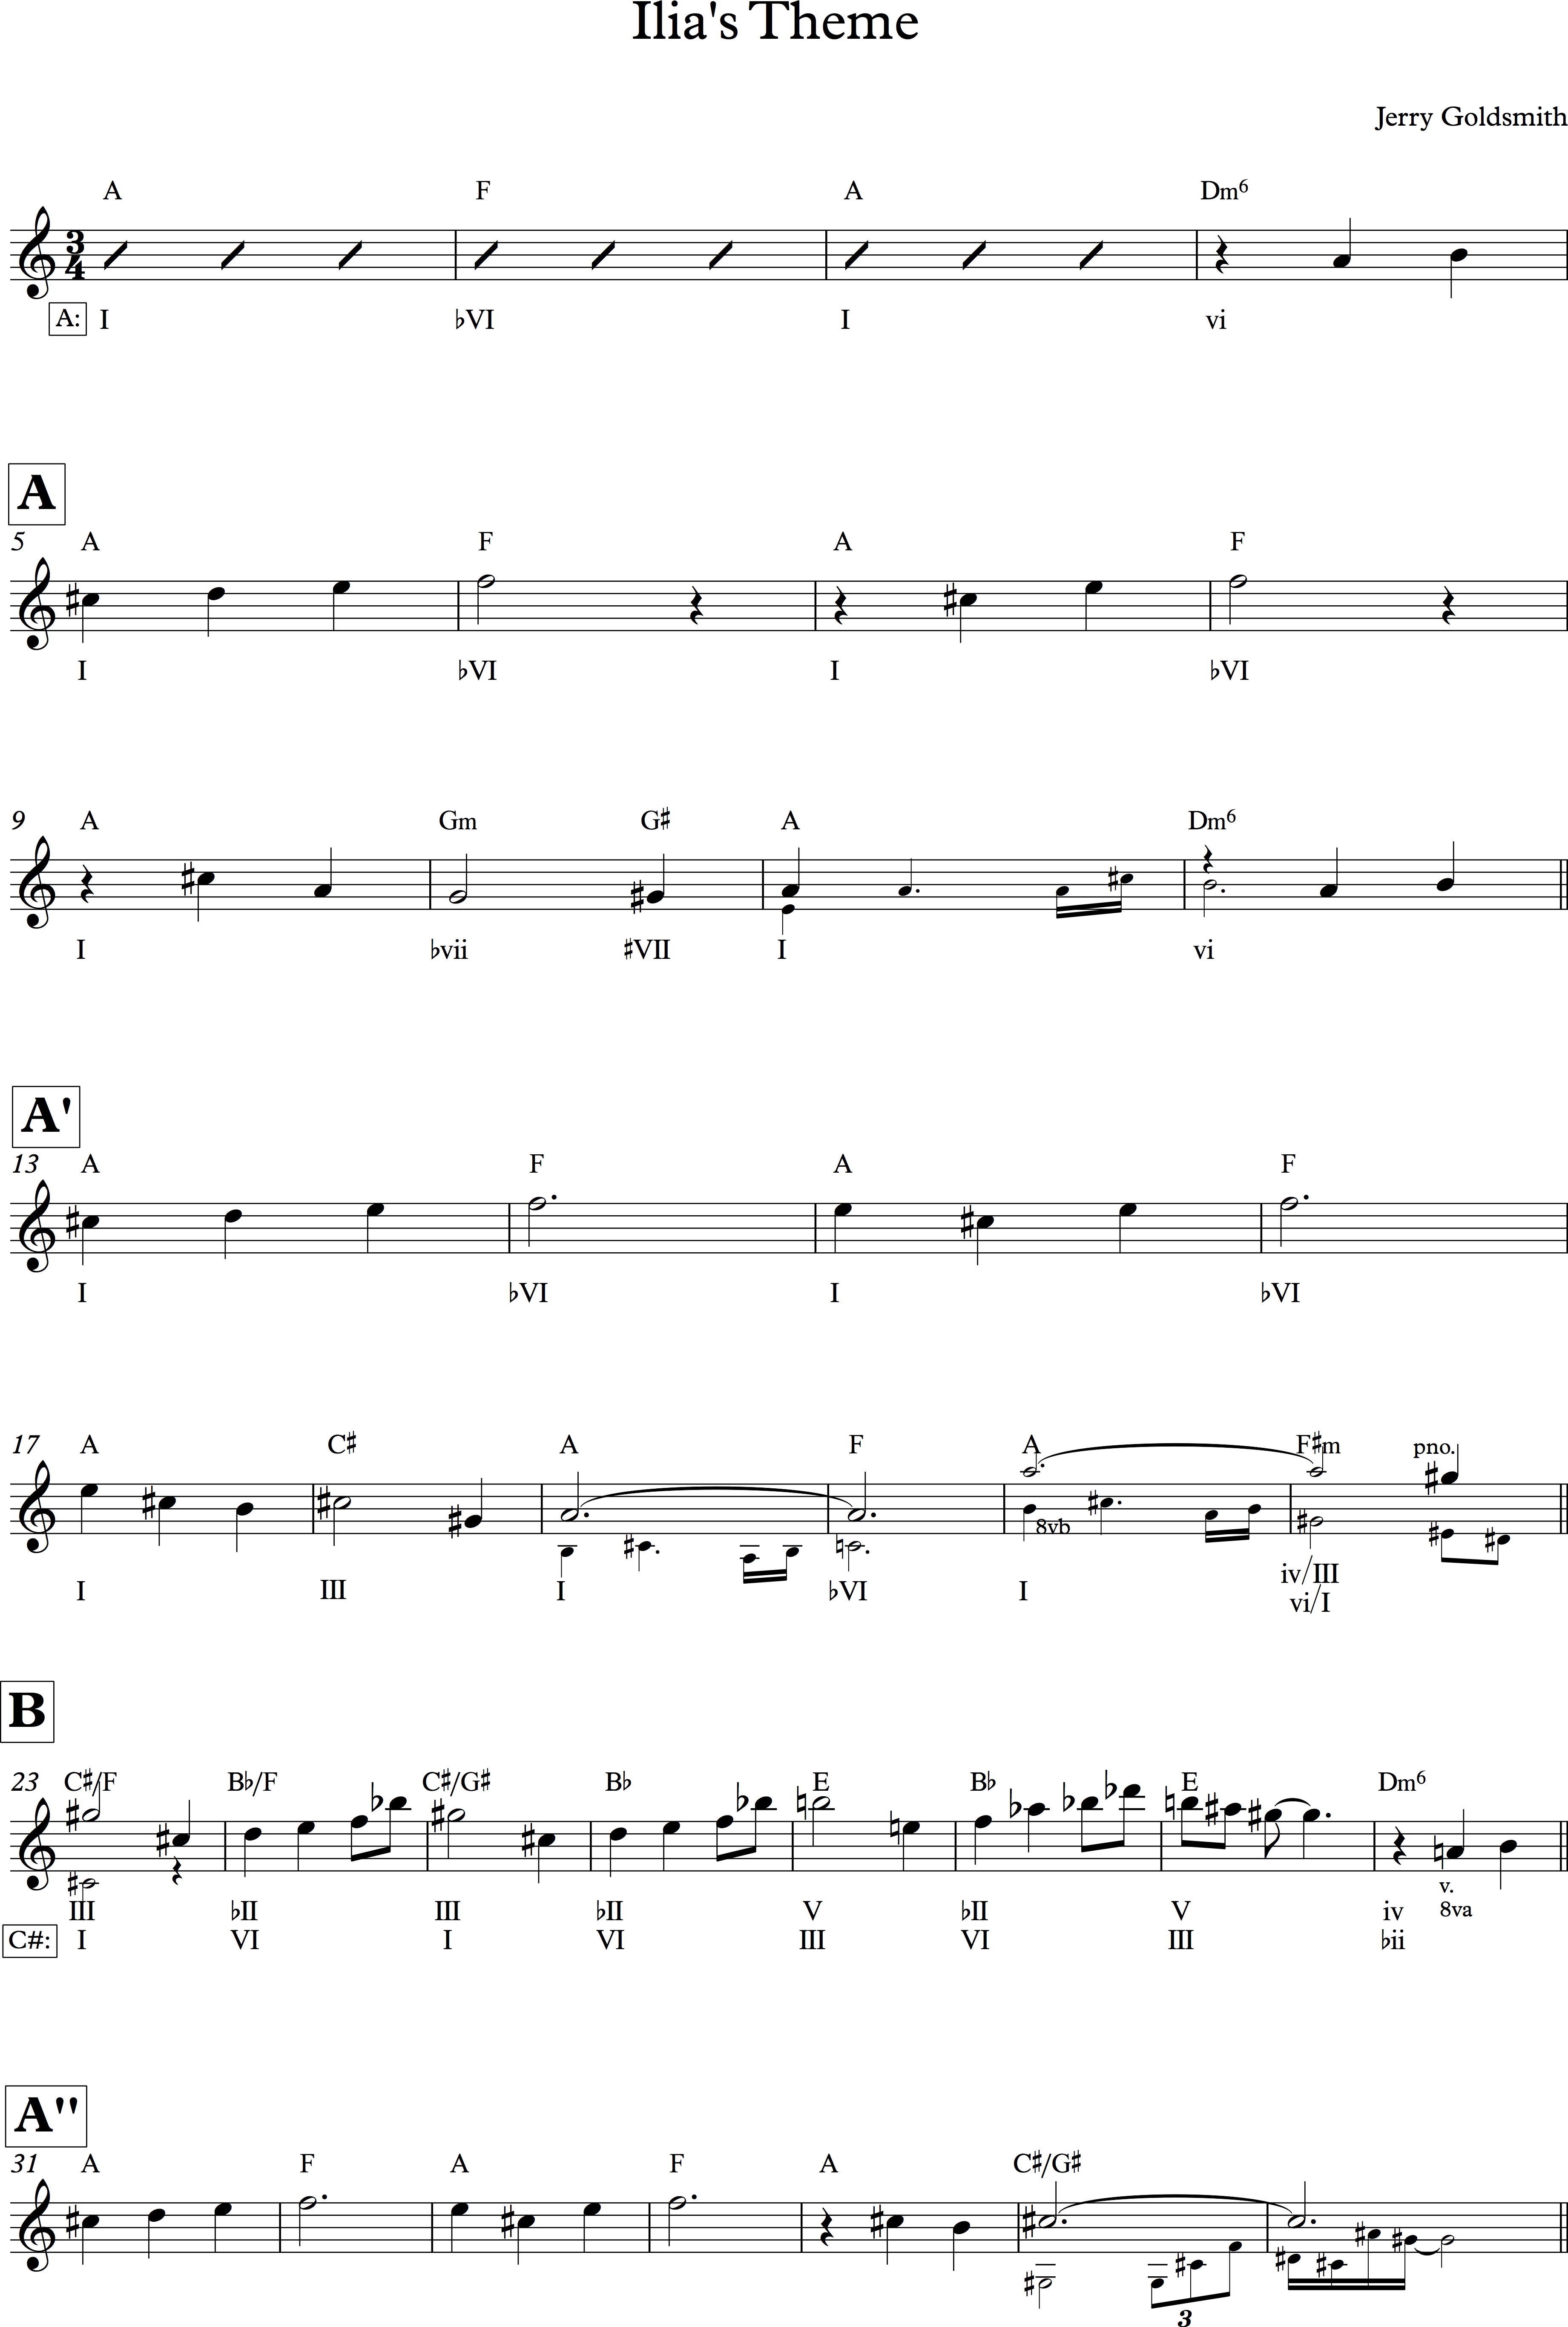
\includegraphics[width=\linewidth]{Ilias_Theme}
	\caption{Ilia's Theme}
	\label{Ilias_Theme}
	\setfloatalignment{b}
\end{figure*} 

\begin{marginfigure}
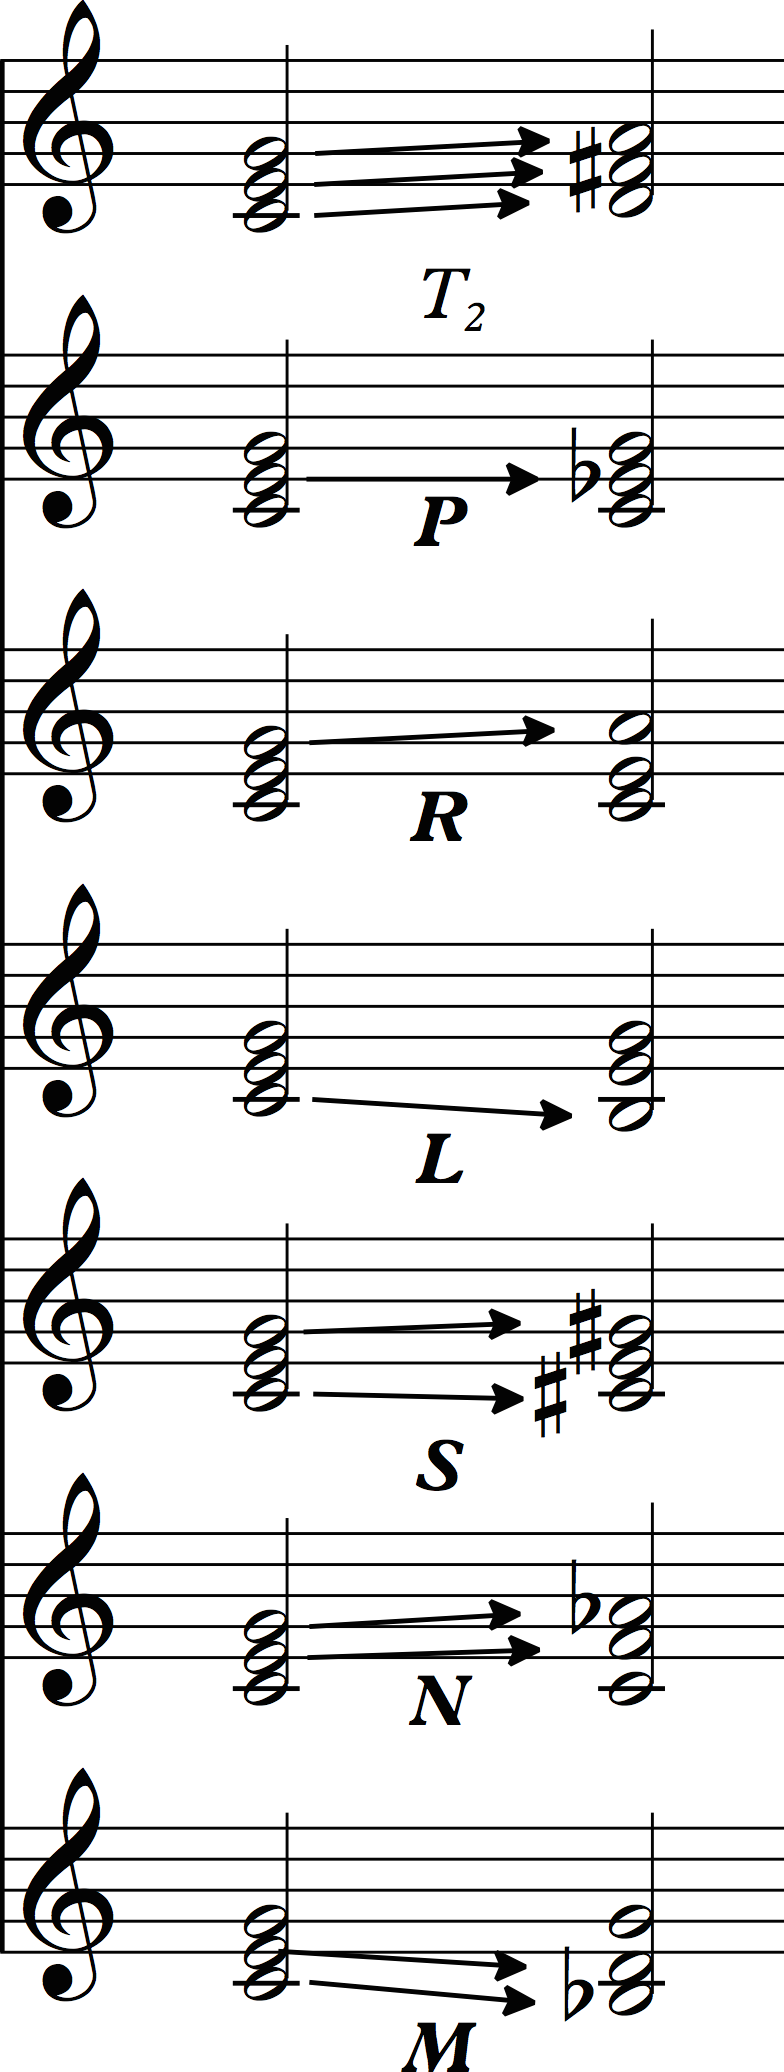
\includegraphics[width=0.7\linewidth]{PRL}
\caption{Basic NRT operators}
\label{fg:prl}
\end{marginfigure}

The main idea of \ac{nRT} is to look at harmonic relations without necessarily relating to a tonic. It does so by looking at how one state changes into another, i.e. \textit{transforms}. It excels as a tool to look for patterns in harmonic progressions otherwise obscured. It is a bit like \textit{Schenker graphs}, but unlike Schenker, \ac{nRT} does not need to work around functional analysis. It does so with tools that look at how a triad \textit{transforms} from one to another. Broken down to its bear essentials \ac{nRT} has three operators that transforms a triad to something else. These are \textbf{(P)arallel}, \textbf{(L)eittonwechsel} and \textbf{(R)elative}. Each operator works both ways; when you have executed [operation] it works in reverse as well. 
\textbf{P} displaces the non-\textit{ic5} pitches in a triad, i.e moves the third between minor and major. For the sake of examples, we assume the first chord in the transformation is \(I\); ergo, in Schenkerian terms it would look like this: \({I}\Leftrightarrow{i}\). 
\textbf{L} displaces non-\textit{ic3} pitches, i.e. the unison in major or the fifth in minor: \({I}\Leftrightarrow{vi}\).
\textbf{R} Displaces the non-\textit{ic4} pitches, i.e the fifth in major and unison in minor: \({I}\Leftrightarrow{vi}\). 
By combining these three operators, it is possible to create \textit{compound operators} and, as such, maneuver from and to each major and minor triad in the 12 tone scale. However, to address some of the more common maneuvers, I will be using a couple of other tools as well. 
\textbf{(S)lide}\footnote{Introduced by \citealt{lewin_generalized_2007}.}, a shorthand for \textbf{L}, \textbf{P} and \textbf{R}, displaces \textit{ic5} pitches, i.e. they move both the prime and fifth: \({I}\Leftrightarrow{\flatx}{ii}\). 
\textbf{(N)ebentonverwandt}\footnote{From Weitzmann via \citealt{lehman_reading_2012}.} displaces the \textit{ic3} pitches, i.e. \({I}\Leftrightarrow{iv}\).  
\textbf{(M)odelverwant}\footnote{Introduced by Frank Lehman in his 2012 dissertation.} displaces ic4 pitches, i.e. \({I}\Leftrightarrow{v}\). I will use \(T_{n}\) to indicate a direct transposition. In addition to the \ac{nRT} operators, I will use diatonic functions as well, indicating \textbf{Tonic}, \textbf{(Dom)inant}, \textbf{(Subd)ominant}, \textbf{(Med)iant} and \textbf{(Subm)ediant} 

\begin{table}
	\small
	\begin{tabularx}{\textwidth}{lll}
		\textbf{Operators}                              				& \textbf{Example}                     	\\ 
		\toprule
		\(T_{n}\): Transpose by \(_{n}\) semitones.    		& \textbf{\(T_{2}\)}\(\Rightarrow\)C=D	\\
		\textbf{P}arallel: Displace non-ic5 pitch       		& \textbf{P}\(\Rightarrow\)C=Cm      	\\
		\textbf{L}eittonwechsel: Displace non-ic3 pitch 		& \textbf{L}\(\Rightarrow\)C=Em      	\\
		\textbf{R}elative: Displace non-ic 4 pitch      		& \textbf{R}\(\Rightarrow\)C=Am      	\\
		\textbf{S}lide: Displace ic5 pitches            			& \textbf{S}\(\Rightarrow\)C=\cissm 	\\
		\textbf{N}ebentonverwandt: Displace ic3 pitches 	& \textbf{N}\(\Rightarrow\)C=Fm      	\\
		\textbf{M}odelverwant: Displace ic4 pitches     		& \textbf{M}\(\Rightarrow\)C=Gm     	\\ 
		\textbf{T}onic								& Chord on scale degree \(\hat{1}\) 	\\
		\textbf{DOM}								& Chord on scale degree \(\hat{5}\)	\\
		\textbf{SUBD}								& Chord on scale degree \(\hat{4}\)	\\
		\textbf{MED}								& Chord on scale degree \(\hat{3}\)	\\
		\textbf{SUBM}								& Chord on scale degree \(\hat{6}\)	\\
		\bottomrule
	\end{tabularx}  
	\caption{Transformational Inventory}
    	\label{tb:transformational_inventory}
\end{table}

%-----------------------------------------------------------------------------
% NRT and Symmetry
%-----------------------------------------------------------------------------
\begin{figure*}[h!]
\texttt{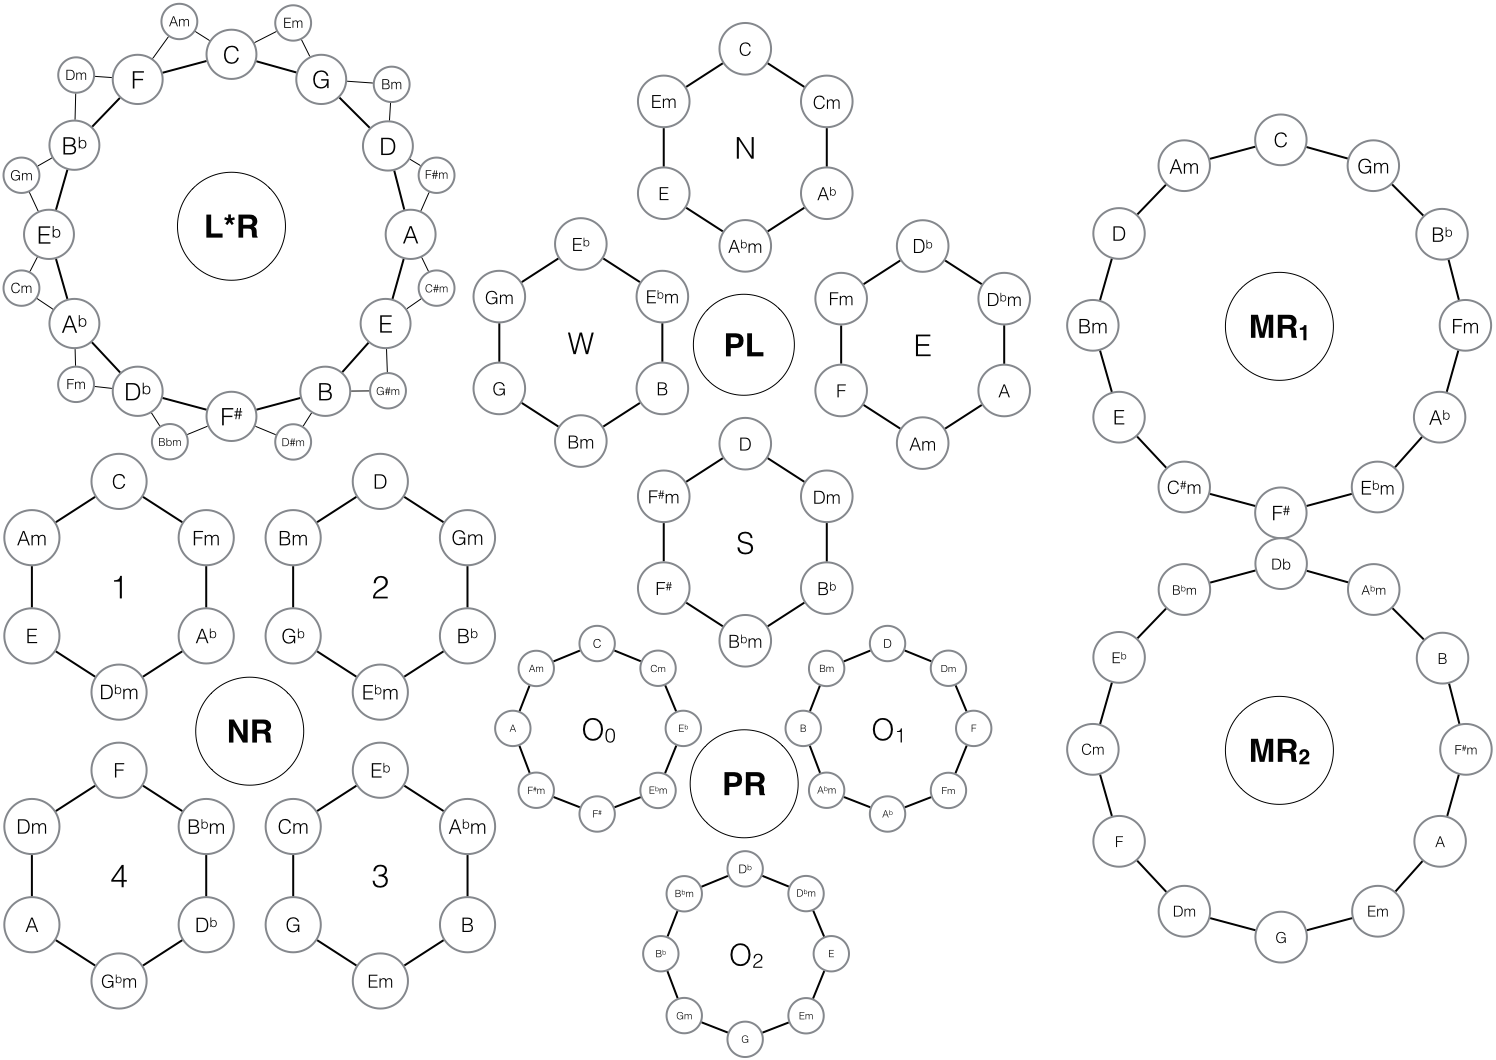
\includegraphics[width=\linewidth]{nrt_circles}
}\caption{neo-Riemannian circles}
\label{fg:nrt_circles}
\end{figure*} 

\section{Symmetry}
Just as we build circles of fifths (\textbf{L\(\cdot\)R}), we can do the same with different combinations of operators, e.g. \textbf{NR}, \textbf{PL}, \textbf{PR} and \textbf{MR}\footnote{It is possible to build other circles, but these are the ones I will use in this thesis}. These circles are what we call \textit{networks}. Each network consists of \textit{nodes} that represent a chord. A collection of networks is called a \textit{hyper system}, for instance, a \textit{hyper octatonic system}. Any given network has a unique name that mirrors the way they were created: \textbf{LR}, \textbf{NR\(_{1-4}\)}, \textbf{PL\(_{n,e,s,w}\)}. \textbf{PR O\(_{0-2}\)} and \textbf{MR\(_{1-2}\)}. In the case of \textbf{NR} and \textbf{PL}, we call them hexatonic networks because they consists of six nodes. It takes four networks to cover the entire major/minor cycle. \textbf{PR} is octatonic and uses three networks to fill the entire major/minor cycle. The \textbf{MR} network uses twelve nodes and requires two networks to complete the entire major/minor cycle. When a progression follows only a progression exclusively in one network, I call it a ``\textit{forced progression}'' and when a progression moves from one network to another, regardless of its parent, it is called a network modulation. In my analysis, these networks will always be displayed with their designators, but not necessarily the parent, for instance \textbf{PL}. Figure \ref{fg:nrt_circles} gives an overview over the networks I will be using. 

\marginnote[-5cm]{The heaxtonic \textbf{PL}, \textbf{PR} and octatonic \textbf{PR} networks are borrowed from Lehman and Lewin's papers and follow the designators used by them.}

	
%-----------------------------------------------------------------------------
% nRT Augmented chords
%-----------------------------------------------------------------------------

\section{Augmented Chords} 

\ac{nRT} was made to address major and minor triads and does so quite brilliantly. It does not, however, handle augmented chords at all. The question thus presents itself: How are augmented chords to be dealt with? One approach is, simply, to indicate that something has happened which could be interpreted with transformational glasses. Frank Lehman postulates an asterisk, \textbf{*}\parencite{lehman_reading_2012}, when dealing with ``near transformational'' moves. This mostly refers to the appearance of tetrachords like \(F{\Rightarrow}C{^7}\) which, in \ac{nRT} terms, translates to \textbf{*LR}. The asterisk tells us that we have not accounted for the added \textit{\flatx7}, but overall, the added note does not affect the main idea. Hugo Riemann's term for this is \textit{''kläng''}. With augmented and diminished chords, however, the \textit{kläng} is altered beyond the point of recognition and function. To show an example on such case that features this problem I refer to figure \ref{fg:sttmp_m.9-10}. The excerpt is from the Overture of \ac{ST:TMP} and shows a pass from \({I}{\Rightarrow}{v}^{\flatx5}\). Here we cannot say we have the same \textit{kläng} when we arrive at \(v\), since the fifth is diminished and there's an added \flatx7. I have chosen not to make new operators for this at this time and will use \textbf{*} to indicate that the root movement is conserved but the \textit{kläng} has been altered. 

\begin{marginfigure}[-4cm]
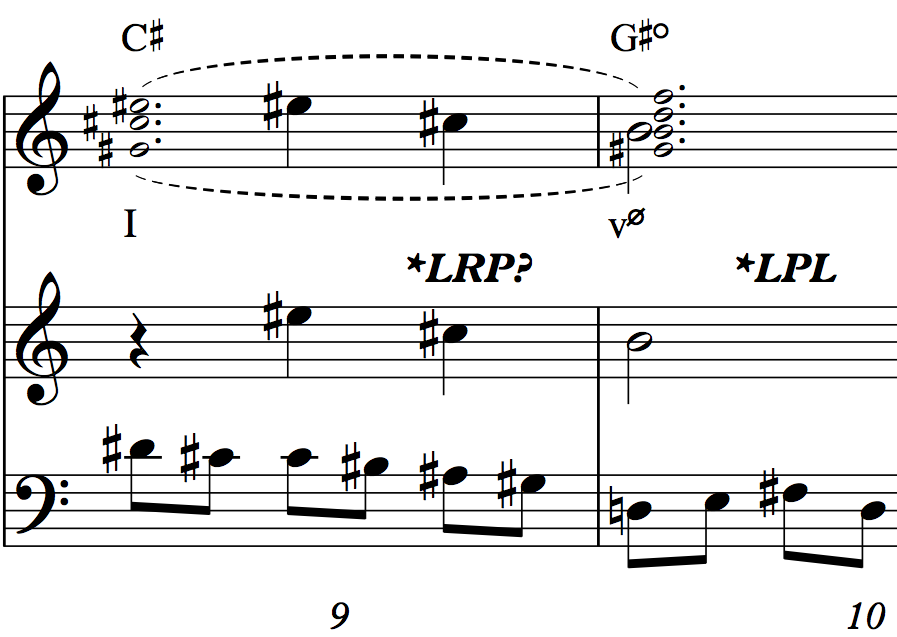
\includegraphics[width=\linewidth]{STTMP_m9-10}
\caption{ST:TMP Overture m. 9-10}
\label{fg:sttmp_m.9-10}
\end{marginfigure}


%----------------------------------------------------------------------------------------
%   Part 2
%----------------------------------------------------------------------------------------
% !TEX root = ../../../Masterthesis.tex

\chapter{Star Trek: The Motion Picture}\label{ch:sttmp}

\section{Overture}
%-----------------------------------------------------------------------------
% Introduction
%-----------------------------------------------------------------------------
\begin{figure}
\center
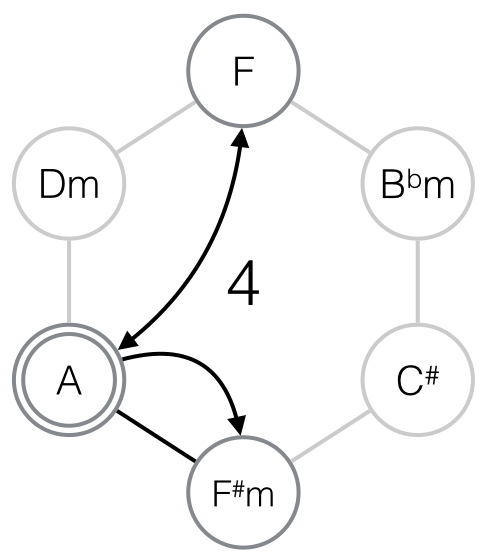
\includegraphics[width=0.5\linewidth]{STTMP_overture_1}
	\caption{ST:TMP: Overture Intro}
	\label{fg:sttmp_overture_1}
\end{figure}

\noindent\newthought{\acf{ST:TMP}} opens to a black screen accompanied by a musical overture. It portrays ''Ilia's Theme'', otherwise know as the ''Love Theme''. It is hard to find a tonic in this piece within the confines of traditional tonal music. However, I do not believe it to be of any consequence since working with film music literature often is about finding the \textit{tonal centre}. In the case of the romantic and string saturated ''Ilia's Theme'' we find the main sections moving around between four pillars; A, \ciss, F and C, each fixated in a hexatonic network. The introduction, figure \ref{fg:sttmp_overture_1} starts with what would seem to be a progression tonally unrelated to the axiom of the song, \ciss, but is in fact part of the same hexatonic \textbf{NR\(_{4}\)} circle. After \(F\sharpx{m}^{6}\Rightarrow{C\sharpx}\), a ''hollywood cadence'', the main theme starts. 
%-----------------------------------------------------------------------------
% A
%-----------------------------------------------------------------------------
\begin{figure}
\center
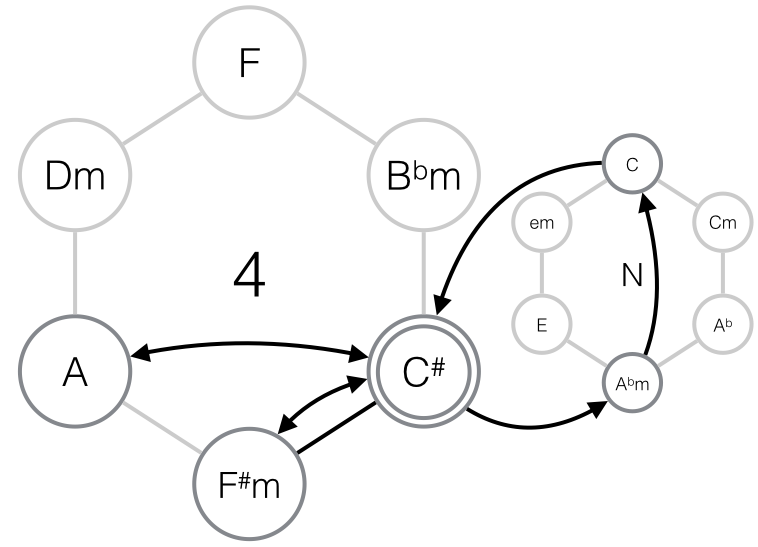
\includegraphics[width=0.7\linewidth]{STTMP_overture_2}
	\caption{ST:TMP: Overture A}
	\label{fg:sttmp_overture_2}
\end{figure}

The main theme of this cue mainly plays out in the \textbf{NR\(_{4}\)} circle. The exception is a network modulation to the \textbf{PL\(_{N}\)} circle. There is an argument to be made for view the \(G\sharpx{m}^{7(\flatx{5})}\), \textit{pc} [036t]\footnote{\keyboard{one=C,two=Diss,three=Fiss,four=Aiss,}}, as a \(E^{9}\)/\giss, but nevertheless, the main body of the chord is a \gissm \textit{transformed} with \(\flatx{5}\) (figure \ref{fg:sttmp_overture_2}).

%-----------------------------------------------------------------------------
% A'
%-----------------------------------------------------------------------------
\begin{figure}
\center
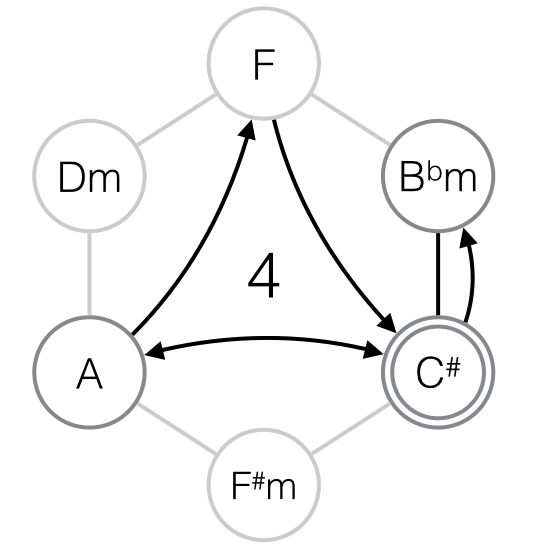
\includegraphics[width=0.5\linewidth]{STTMP_overture_3}
	\caption{ST:TMP: Overture A'}
	\label{fg:sttmp_overture_3}
\end{figure}
The second pass of A, figure \ref{fg:sttmp_overture_3}, works much in the same way, but instead of modulating outside the \textbf{NR\(_{4}\)}, Goldsmith does a minor transformation on the melody, \textbf{m.}17-18, making room for a simple \textbf{LP} to F\footnote{Which might be seen as a projection to the following part.}. The part ends with a \aissm, making it the new \(iv\), another ''hollywood cadence''. 

%-----------------------------------------------------------------------------
% B
%-----------------------------------------------------------------------------
\begin{figure}
\center
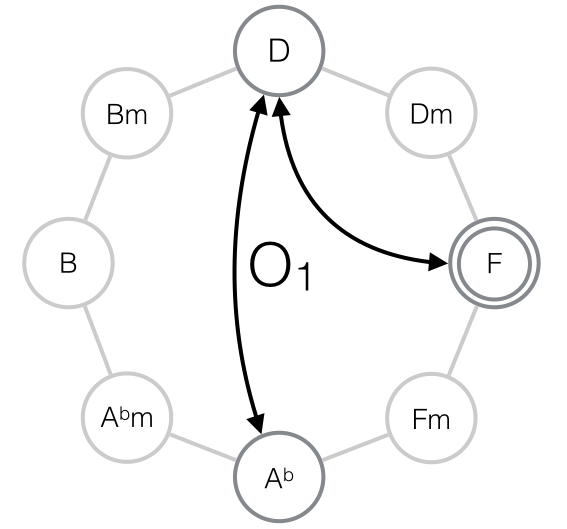
\includegraphics[width=0.5\linewidth]{STTMP_overture_4}
	\caption{ST:TMP: Overture B}
	\label{fg:sttmp_overture_4}
\end{figure}
The second part, and theme (figure \ref{fg:sttmp_overture_4}), of the cue is entirely situated in \(O_{1}\). With a pedal A acting as a coupling between F and D, acting as \(\hat{3}\) and \(\hat{5}\), Goldsmith activates a melody with a \textit{lydian} tinge before deploying a \ac{MTTP}, now famously associated with space\footnote{A term borrowed from Scott Murphy \citet{murphy_major_2006}. This progression to be treated in greater detail as I progress through this text.}.


%-----------------------------------------------------------------------------
% A''
%-----------------------------------------------------------------------------
\begin{figure}
\center
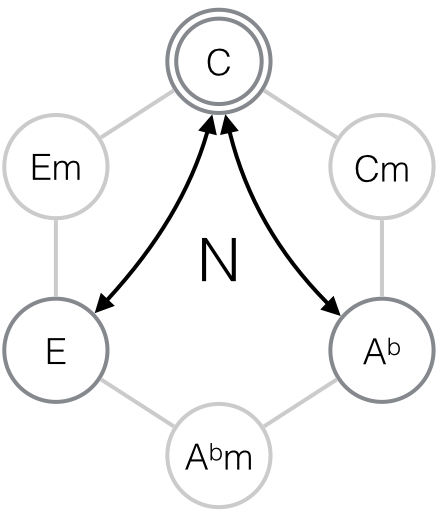
\includegraphics[width=0.5\linewidth]{STTMP_overture_5}
	\caption{ST:TMP: Overture A''}
	\label{fg:sttmp_overture_5}
	\setfloatalignment{b}
\end{figure}
When Goldsmith returns to the main theme, figure \ref{fg:sttmp_overture_5}, it is transposed to from \aflat to C, making yet another mediant modulation. The harmony is rooted in C with a pedal G. The melody uses \(\flatx{6}\), hinting at a mixolydian \(\flatx{6}\), the fifth mode in melodic minor. Through yet another mediant modulation to E Goldsmith executes the outro.


%-----------------------------------------------------------------------------
% Outro
%-----------------------------------------------------------------------------
The Outro, figure \ref{fg:sttmp_overture_6}, is a proto-projection of the now famous ''Enterprise Theme'' composed by Alexander Courage. The cadence: \(I-{\flatx}VII-IV-I\) is a \emph{subtonic plagal cadence} and is reminiscent of the old ''spaghetti'' westerns, which frequently use the \emph{subtonic half cadence}: \(I-{\flatx}VII-V-I\)\footnote{\citealt{lehman_hollywood_2013}}. It serves two purposes: (1) to project and prepare the enterprise theme and (2) to prepare the overall sonority for the main title.

\begin{figure}
\center
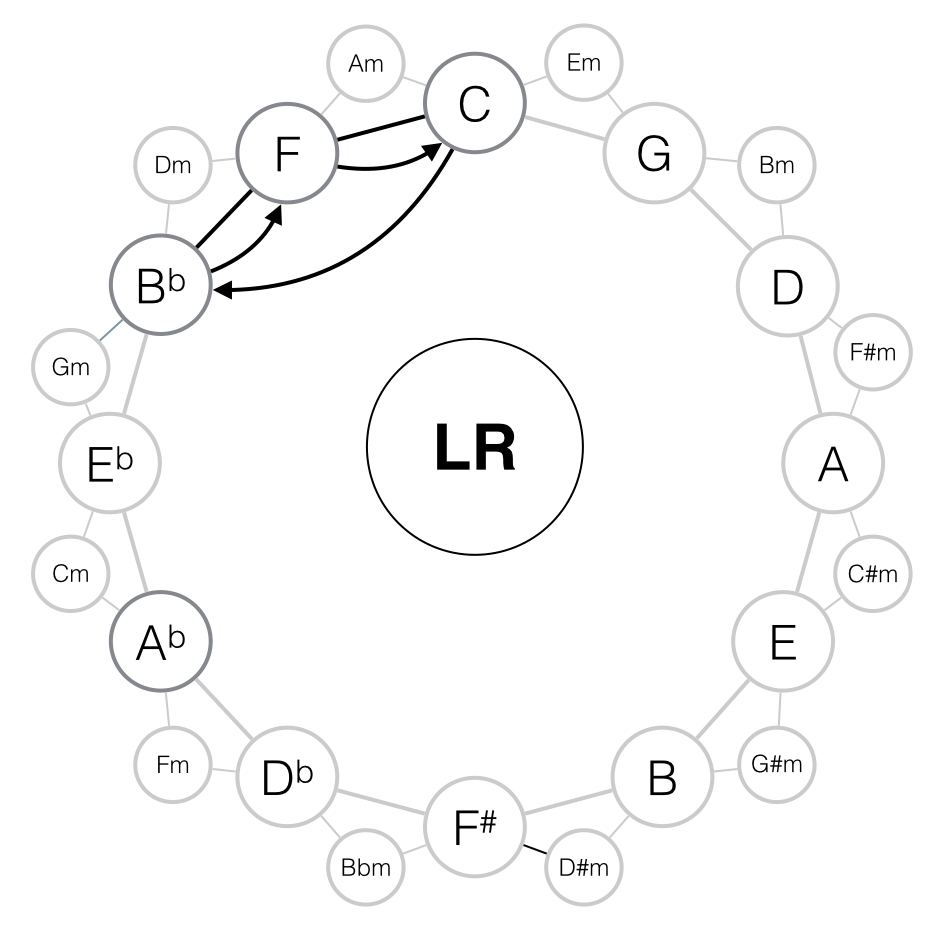
\includegraphics[width=0.7\linewidth]{STTMP_overture_6}
	\caption{ST:TMP: Overture Outro}
	\label{fg:sttmp_overture_6}
\end{figure}

%-----------------------------------------------------------------------------
% PDF
%-----------------------------------------------------------------------------
\clearpage
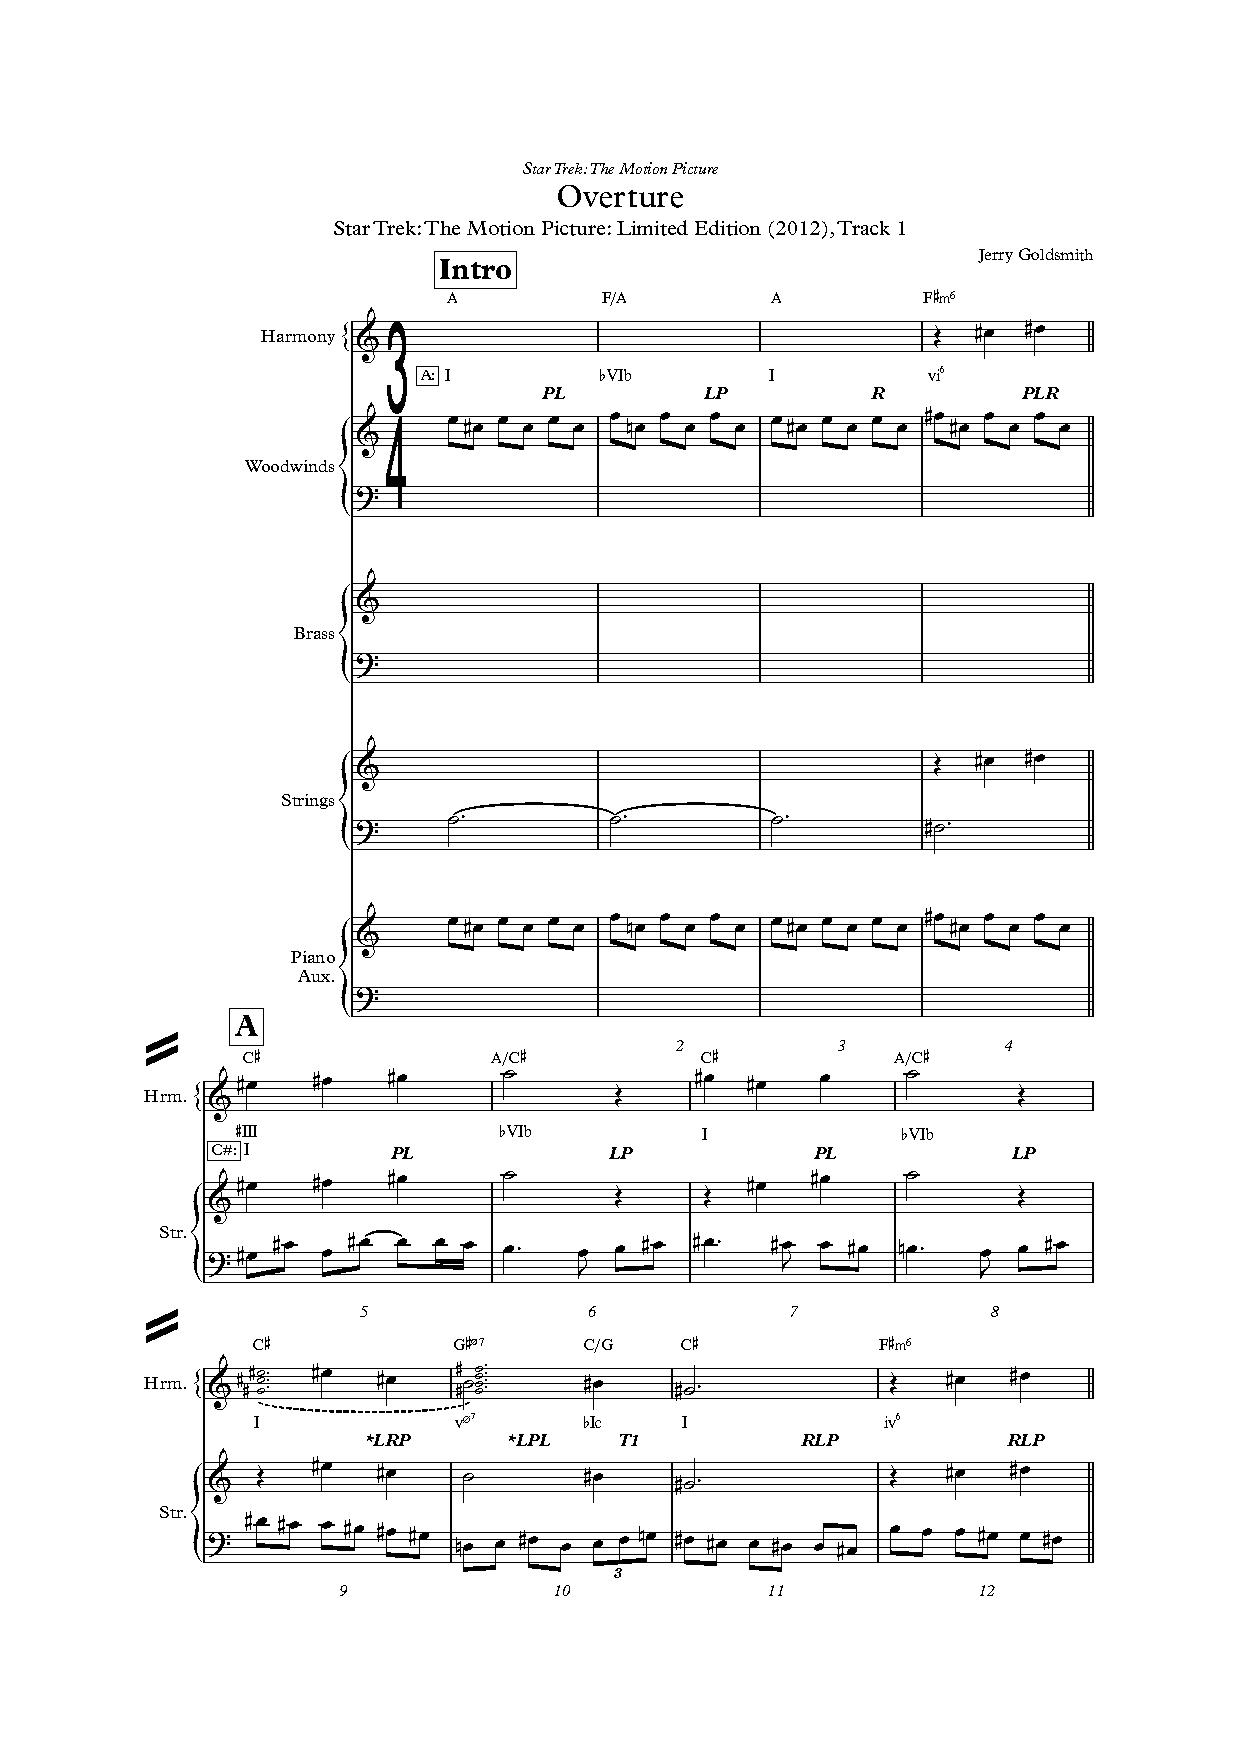
\includepdf[pages=-,pagecommand=\thispagestyle{fancy}]{pdf/st1/STTMP_Overtyre.pdf}

% Reviewed
% !TEX encoding = UTF-8 Unicode
% !TEX root = ../../../Masterthesis.tex
\section{Main Title}\label{sec:STTMP Main Title}
%-----------------------------------------------------------------------------
% Intro
%-----------------------------------------------------------------------------
\begin{figure}[h!]
\center
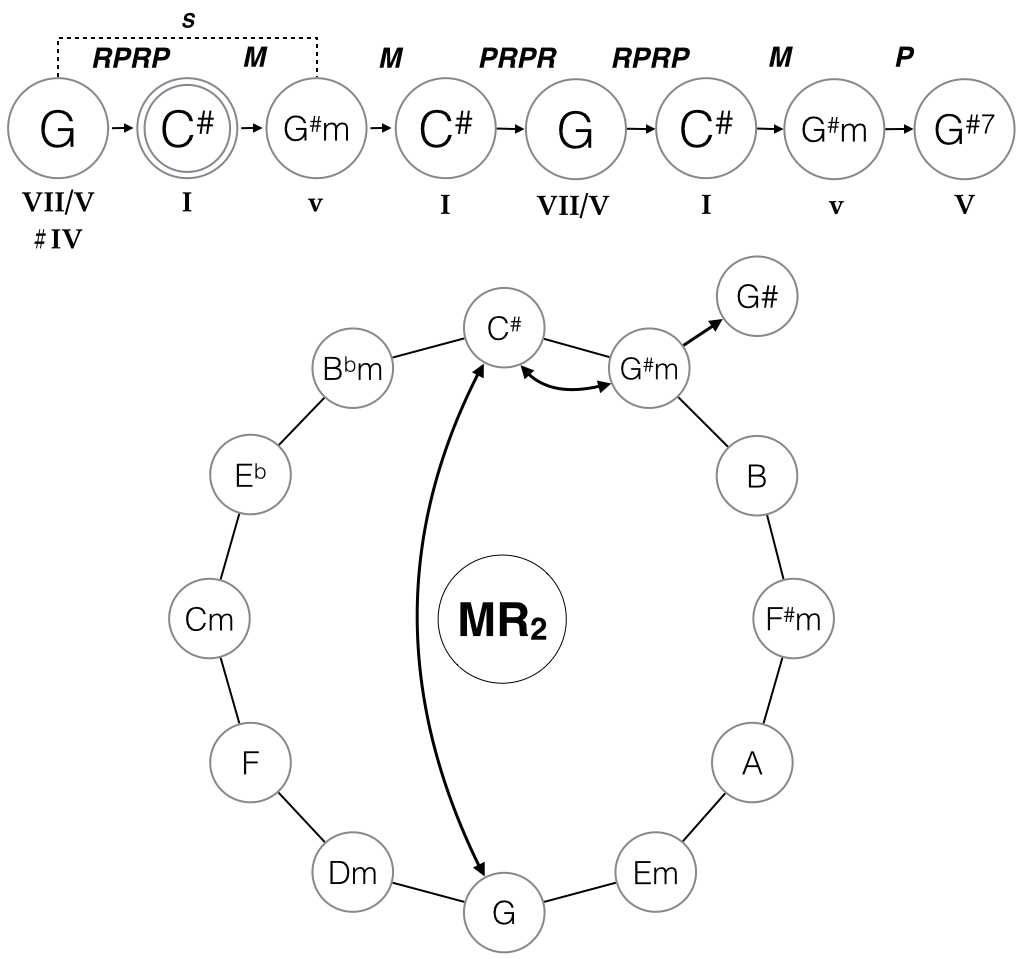
\includegraphics[width=\linewidth]{STTMP_Main_Title_intro}
	\caption{ST:TMP: Main Title Intro}
	\label{fg:sttmp_main_title_intro}
	\setfloatalignment{b}
\end{figure}

\noindent The music starts with the Paramount logo, and music is played with the opening credits. The form is reminiscent of a Rondo, where the overall structure is ABABA, containing development parts.
In figure \ref{fg:sttmp_main_title_intro}, we see that the first two chords in this main title tell us quite a few things. First of all, the relation between them are a tritone, and the G does not seem to be the tonic. The \acf{MTTP} in science fiction movies have been around since the 1950's\parencite{murphy_major_2006} and the origins of tritone progression related to something extraterrestrial is generally believed to stem from Holst's: The Planets,\footnote{Mars: Strings play col legno in 5/8, while the brass plays the main motif: [0,7,6]  bringing the tritone into play as the harbinger of death; Mars, the God of War.} thus signifying both the monstrous\parencite{fairweather_jerry_2014} and outer space. By executing this from the very beginning, he implicitly states that this tale will not necessarily happen on earth and, at the very least, contains imagery depicting something outer-wordly, i.e. there will be a monster in some form or another. 

The G in this progression poses a challenge to traditional tonal thinking, and if one assumes G as tonic the rest that follows is, at best, very unstable. The \ciss seems to carry the majority of tonic weight. The G in the context of \ciss could be interpreted as either \(\sharp{IV}\) or \(VII/V\) but both cloud the musical intention. \gissm could be considered a mixolydian \(v\) thus making a \textbf{S} relationship with G. The cadence is, thanks to the \giss, acting as a \(({\flat}VII)\) subtonic cadence to \bflat giving a nod to the musical practices in established in Western's between 1920 and 1940.
\marginnote[-4cm]{
Frank Lehman's essay on ``Hollywood Cadences'' tells us this type of cadence is common with the practices found in Westerns and its sub-genres. This provides a clue to what we can expect. Roddenberry himself has called Star Trek a ``space western'' and the cadences used are evidence of this: \textquote[\cite{lehman_hollywood_2013}]{The cadence€™s capacity to index film genre is as potent as its ability to punctuate and structure dramatic action.}
}

%-----------------------------------------------------------------------------
% A and A' 
%-----------------------------------------------------------------------------
Figure \ref{fg:sttmp_main_title_a}, A shows that the main theme is situated harmonically around fifths. The tonality is clearly mixolydian with evidence enclosed in the minor \(v\). The sublime references to ``cowboy music'' keeps recurring with the oscillating \(I \Leftrightarrow \flat{VII}\). The part repeats and ends on F. I have also provided a simple \textit{Tonnetz} graph\footnote{Blue is minor and Red is major.} of the passage to show that it is possible to discern a pattern using this. It is, however, not something I will continue to use as is to obscure in its reading. 

\begin{figure*}
\center
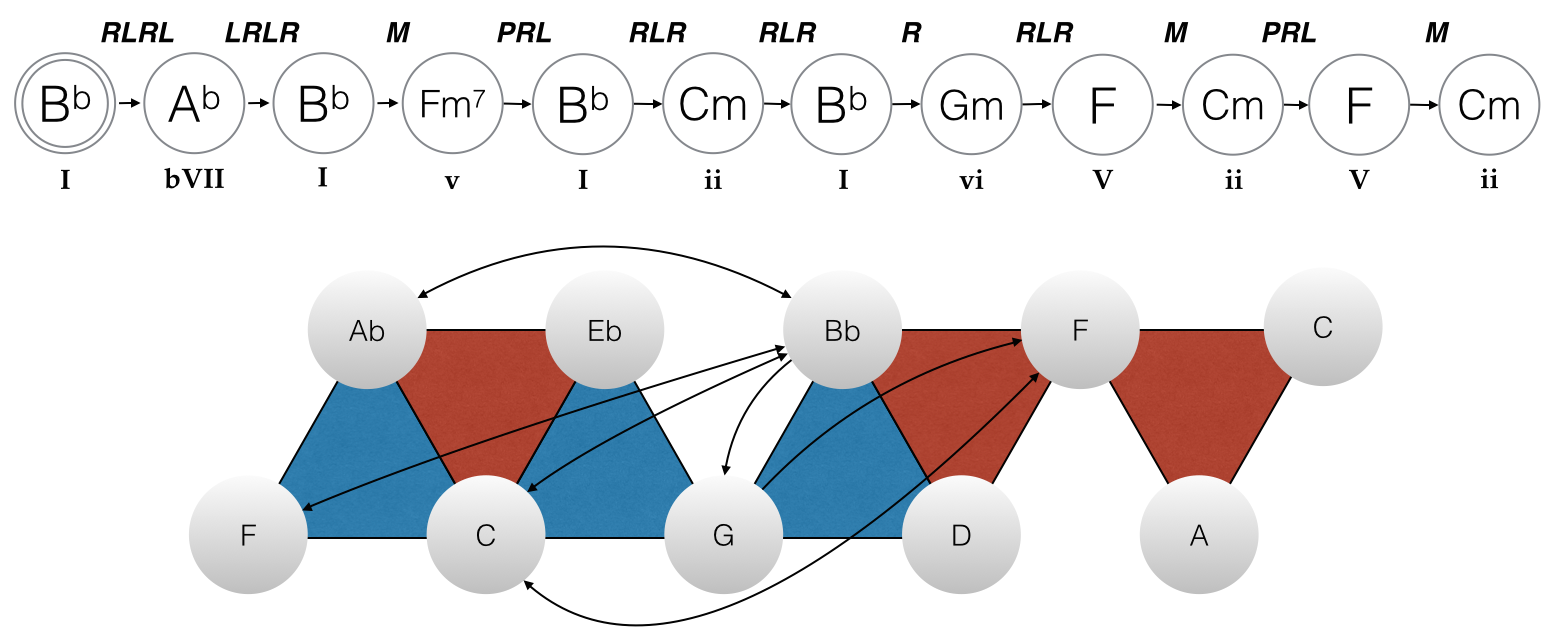
\includegraphics[width=\linewidth]{STTMP_Main_Title_A}
	\caption{ST:TMP: Main Title A}
	\label{fg:sttmp_main_title_a}
\end{figure*}


%-----------------------------------------------------------------------------
% B and B'
%-----------------------------------------------------------------------------
\begin{figure}[h!]
\center
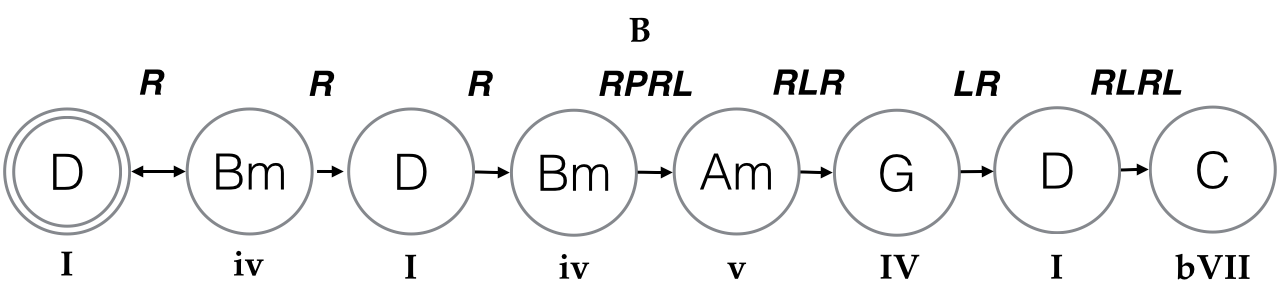
\includegraphics[width=\linewidth]{STTMP_Main_Title_B}
	\caption{ST:TMP Main Title B}
	\label{fg:sttmp_main_title_b}
	\setfloatalignment{b}
\end{figure}

The entrance to B, figure \ref{fg:sttmp_main_title_b}, is via F, which acts as (\(\flat{III}\)) in the new tonic making it a \textit{type 2} flat mediant modulation\parencite{lehman_hollywood_2013} seen both from the tonic D and F. The music is still saturated in mixolydian scale, providing both the minor \(v\) and the \(bVII\).

\begin{figure}[h!]
\center
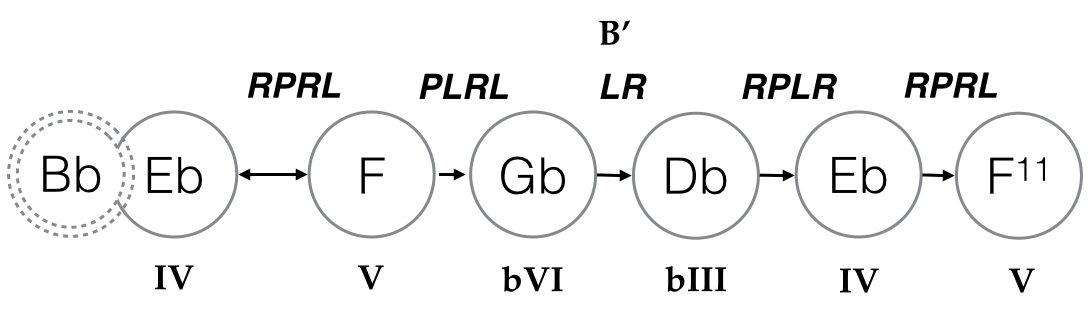
\includegraphics[width=\linewidth]{STTMP_Main_Title_B'_1}
	\caption{ST:TMP: Main Title B' 1}
	\label{fg:sttmp_main_title_b_1}
	\setfloatalignment{b}
\end{figure}

B' starts with the modulation from the previous C/D  to \eflat. The C/D, in this case, acts as bVII in D, but if one would think it as a \textbf{Dominant} in G: D\(^{11}\), in relation to \eflat it provides a \textit{deceptive cadence}, making the formula: \(V(D^{11})\Rightarrow{\flat}VI(E{\flat})\). But the tonal trickery does not stop there. Goldsmith makes \eflat to be \(IV\), making the key \bflat. The evidence for that lies in the cascading cadences that follow. If F is \(V\) then its connections to the other chords can be seen in figure \ref{fg:sttmp_main_title_b_cadence}. Every one of those connections seen individually and in relation to F is tried and true. What is unusual, is that instead of doing one of them, Goldsmith unleashes a string of them, making a circular modulating network.

\begin{figure}[h!]
\center
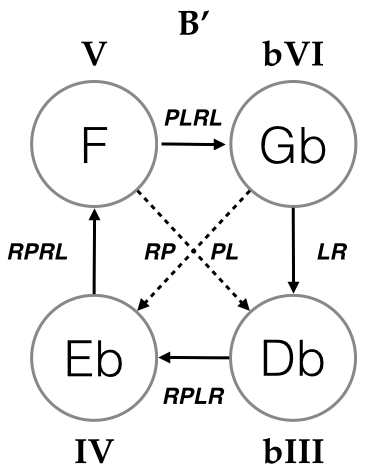
\includegraphics[width=0.4\linewidth]{STTMP_Main_Title_B'_2}
	\caption{ST:TMP: Main Title B' cadence}
	\label{fg:sttmp_main_title_b_cadence}
\end{figure}



%-----------------------------------------------------------------------------
% A''
%-----------------------------------------------------------------------------
\begin{figure}[h!]
\center
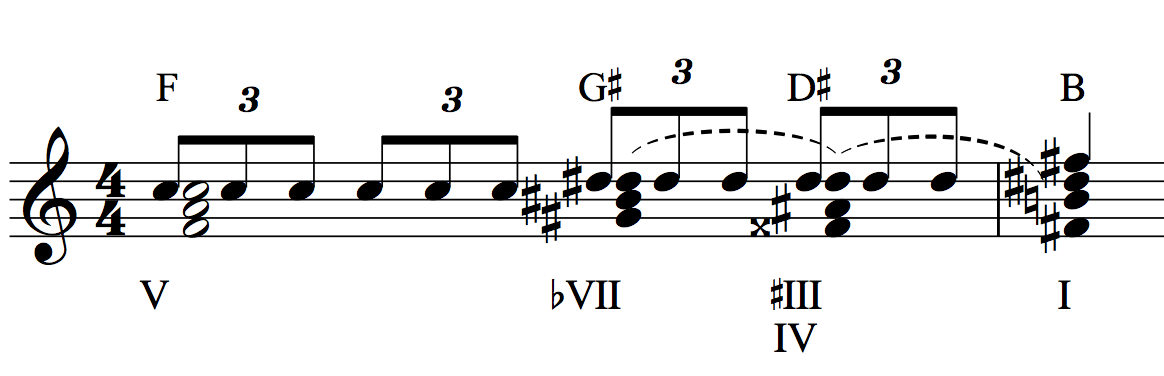
\includegraphics[width=\linewidth]{STTMP_Main_Title_A''}
	\caption{ST:TMP: Main Title A'' cadence}
	\label{fg:sttmp_main_title_a''_cadence}
	\setfloatalignment{b}
\end{figure}

So far the overall structure has been: Intro, A, A', B, B' and now A returns mostly identically to previous iterations, breaking the mold with only one repetition (figure \ref{fg:sttmp_main_title_a''_cadence}).The modulation in m.24 works through three chords sharing one common tone, thus making the maximal usage of one tone to serve as a modulation catalyst, \giss: \(\hat{5}\), \diss: \(\hat{1}\) and B: \(\hat{3}\). Even though the key is \bflat, the relation between F and B is a \ac{MTTP}, further solidifying its position in the Star Trek universe. 

%-----------------------------------------------------------------------------
% B''
%-----------------------------------------------------------------------------
\begin{figure}[h!]
\center
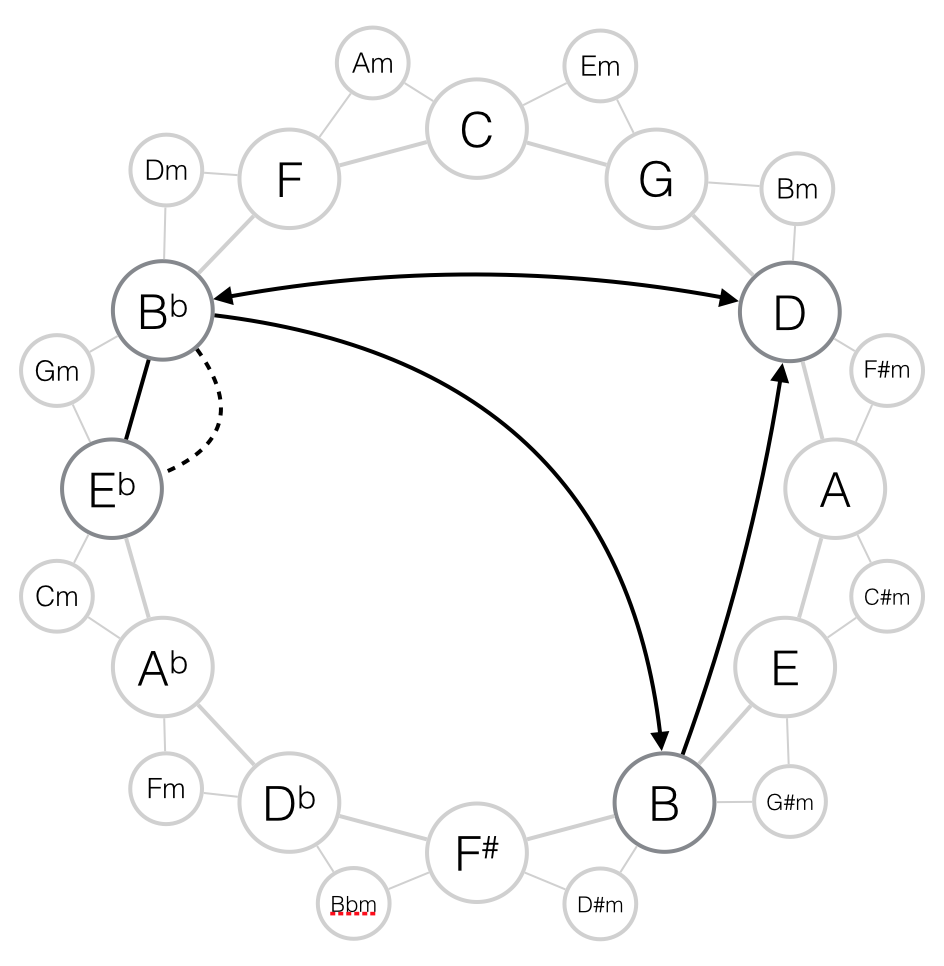
\includegraphics[width=0.7\linewidth]{STTMP_Main_Title_AB_modulation_chart}
	\caption{ST:TMP: Main Title AB modulation chart}
	\label{STTMP_Main_Title_AB_modulation_chart}
	\setfloatalignment{b}
\end{figure}

With the reintroduction of B'', we see that the melody is slightly more relaxed and the modulation formula has changed. When looking at figure \ref{STTMP_Main_Title_AB_modulation_chart} one sees that the modulation described in \ref{fg:sttmp_main_title_a''_cadence} has carried the tonal center further away from \bflat than in previous modulations. The transition from B'' to B''' also follows a different formula; instead of returning to \bflat, Goldsmith modulates to D. 

%-----------------------------------------------------------------------------
% B'''
%-----------------------------------------------------------------------------
\begin{figure}[h!]
\center
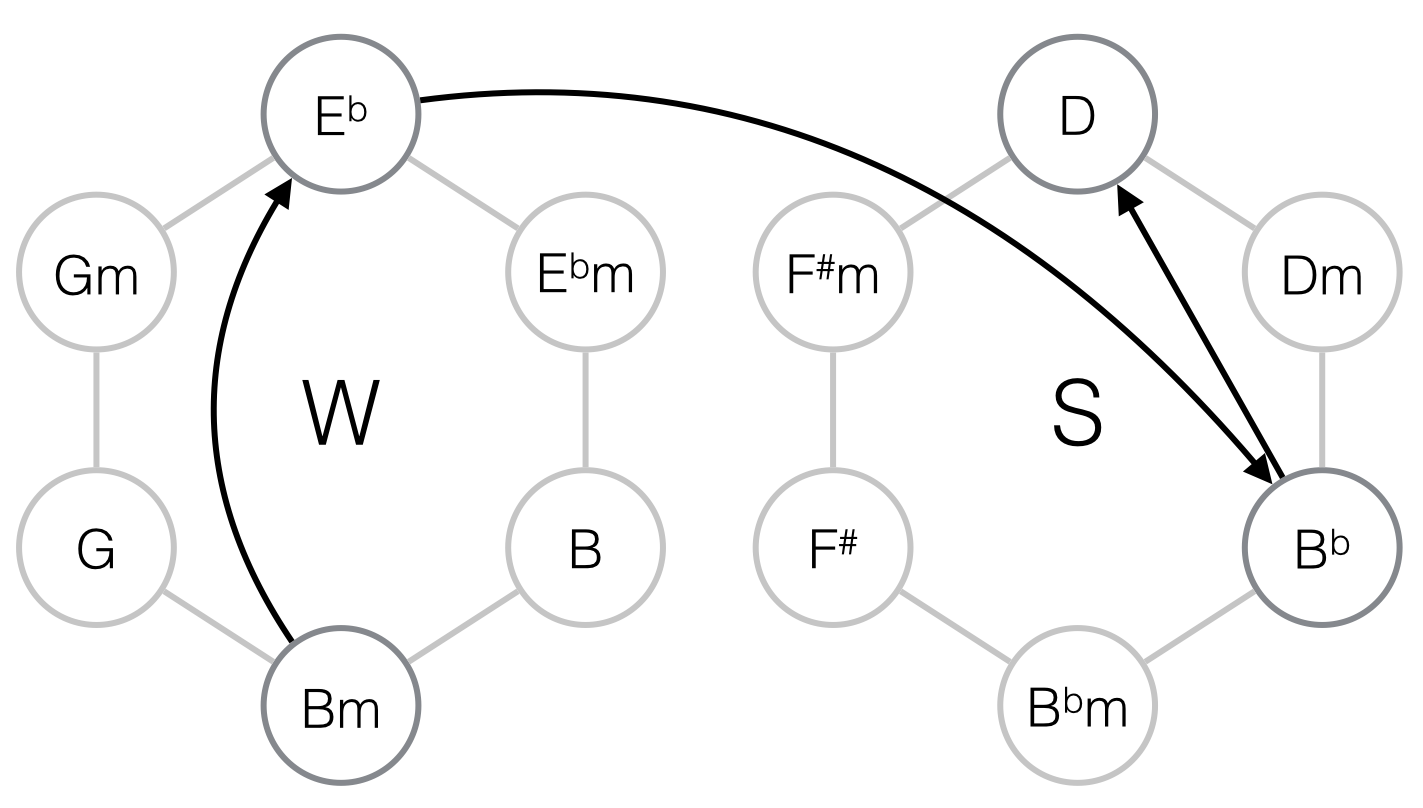
\includegraphics[width=\linewidth]{STTMP_Main_Title_B'''}
	\caption{ST:TMP: Main Title B'' cadence}
	\label{fg:sttmp_main_title_b''_cadence}
	\setfloatalignment{b}
\end{figure}

The four bars of B''' has a solid C pedal over D and the tonality is clearly lydian. The modulation in m.31-32 is possible to view in the \textbf{PL} structures, see figure \ref{fg:sttmp_main_title_b''_cadence}. 

%-----------------------------------------------------------------------------
% A'''
%-----------------------------------------------------------------------------
The final A''' works over a mixolydian G pedal and finishes with a \textit{Aeolian Cadence}, \(\flat{VI}-\flat{VII}\). Overall, the tonality is traceable through the octatonic circles and figure \ref{STTMP_tonal_overview} gives a summary of this.

\clearpage
\begin{figure}
\center
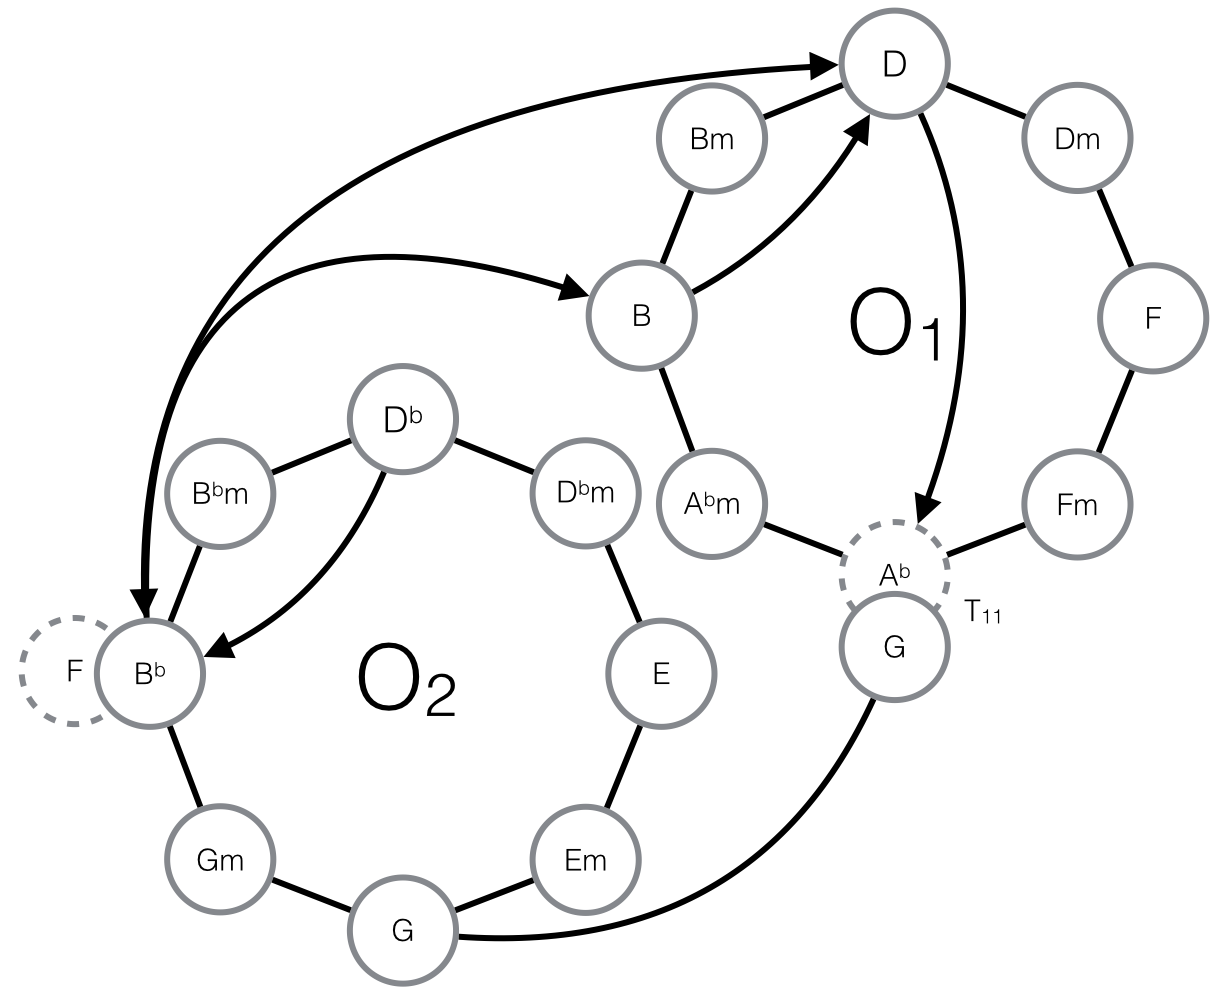
\includegraphics[width=\linewidth]{STTMP_tonal_overview}
	\caption{ST:TMP: Tonal overview}
	\label{STTMP_tonal_overview}
	%\setfloatalignment{b}
\end{figure}


%-----------------------------------------------------------------------------
% PDF
%-----------------------------------------------------------------------------
\clearpage
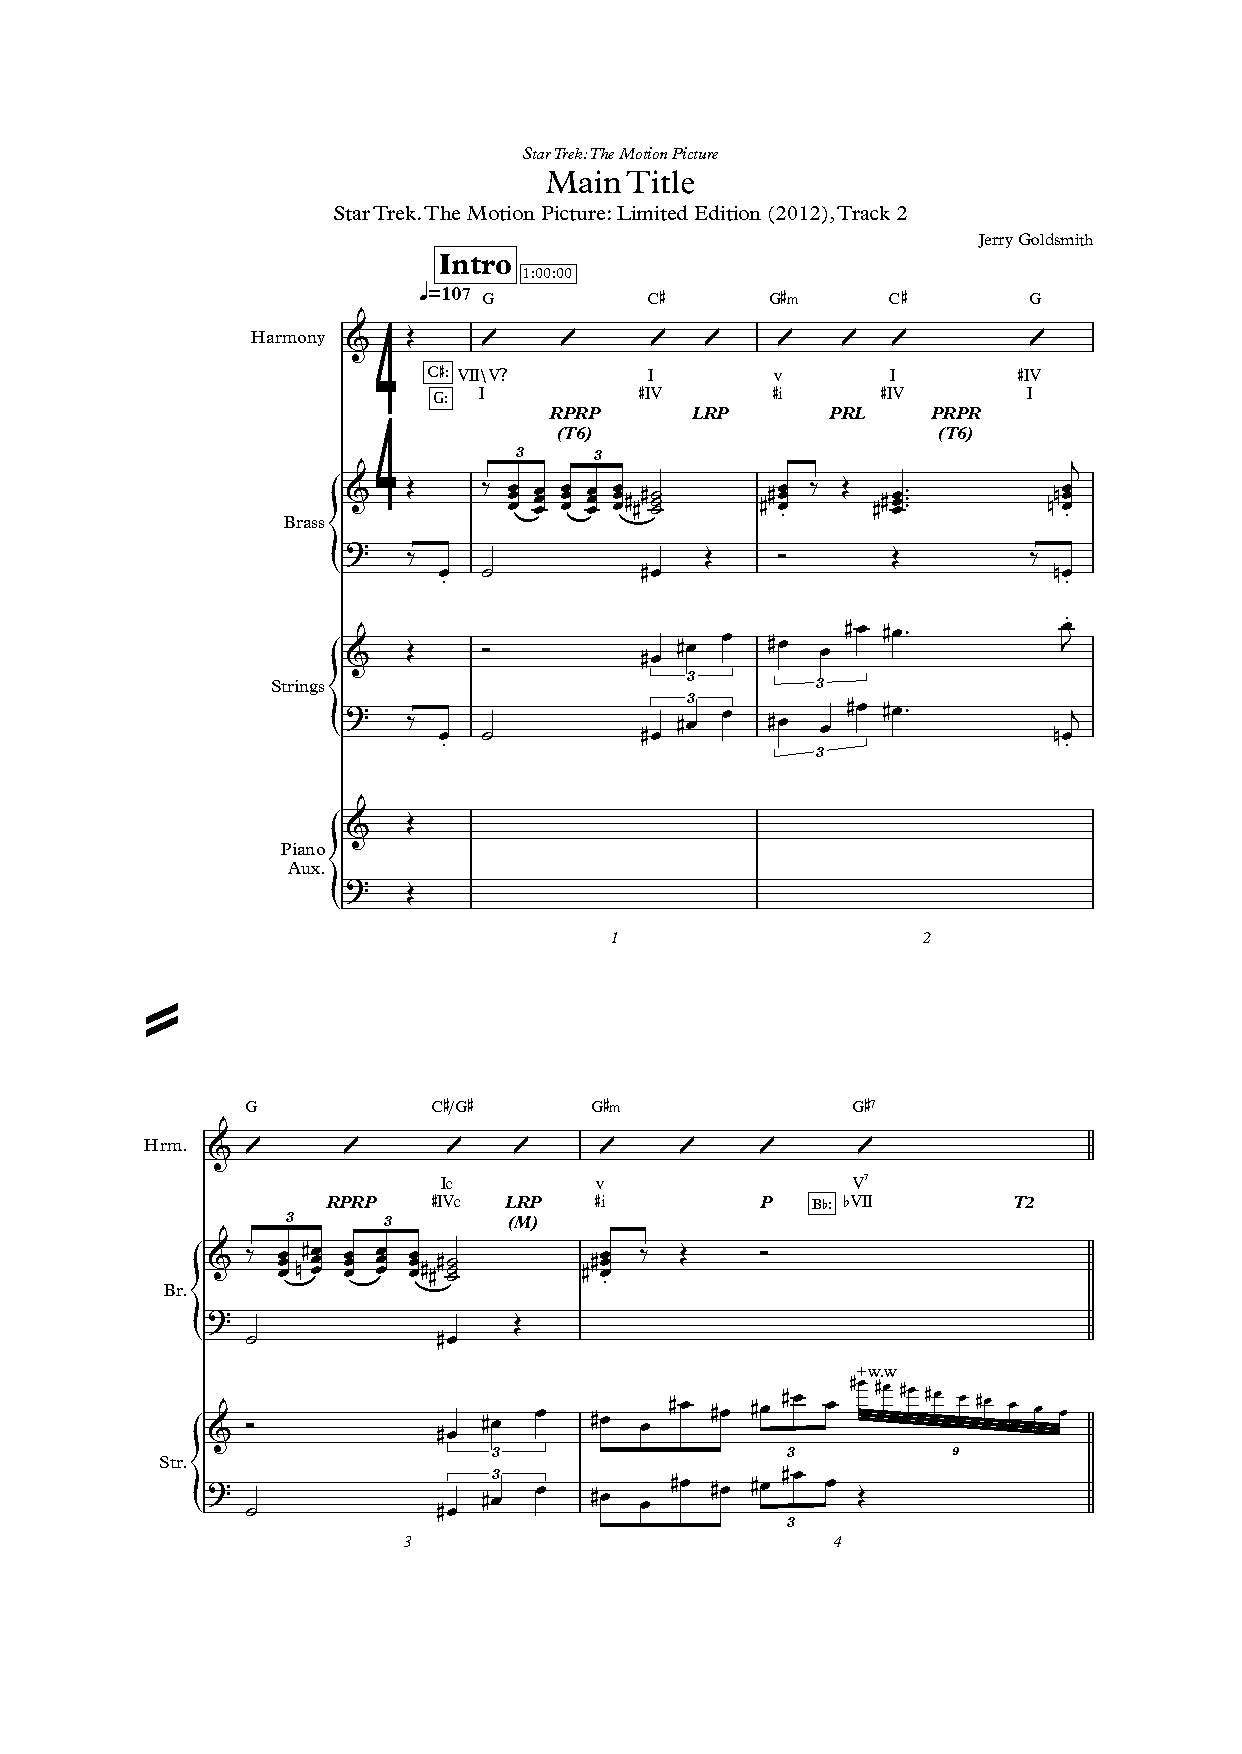
\includepdf[pages=-,pagecommand=\thispagestyle{fancy}]{pdf/st1/STTMP_Main_Title.pdf}

% Reviewed
% !TEX root = ../../../Masterthesis.tex
\section{Leaving Drydock}\label{sec:leaving drydock}
%-----------------------------------------------------------------------------
% A
%-----------------------------------------------------------------------------
\begin{figure*}[h!]
\center
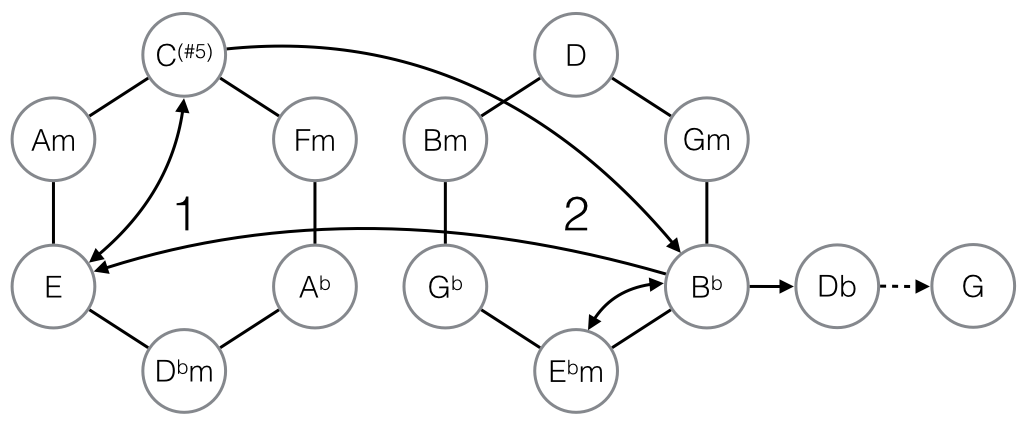
\includegraphics[width=\linewidth]{STTMP_Leaving_Drydock_A}
	\caption{ST:TMP: Leaving Drydock A}
	\label{STTMP_Leaving_Drydock_A}
	%\setfloatalignment{b}
\end{figure*}

\noindent With every crew post now filled, the Enterprise prepares to leave drydock. The music provides an underscore that builds on the tension and excitement that both crew and audience would feel. The time is \lilyTimeSignature{6 + 3}{8 + 4} creating a 3:2 displacement, which Goldsmith uses as a musical device throughout. Goldsmith uses \textbf{N}, thirds and \acf{MTTP}'s to build progressions. See figure \ref{STTMP_Leaving_Drydock_A}. On a few occasions, he uses altered chords and when he does use altered chords there is most likely a \textit{common tone junction} (figure \ref{STTMP_Leaving_Drydock_A2}) binding them together. 

\begin{marginfigure}
%\center
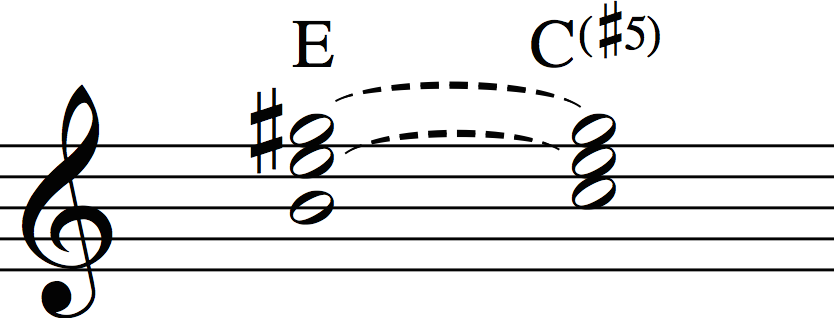
\includegraphics[width=\linewidth]{STTMP_Leaving_Drydock_A2}
	\caption{ST:TMP: Leaving Drydock A: Common Tones}
	\label{STTMP_Leaving_Drydock_A2}
	%\setfloatalignment{b}
\end{marginfigure}

%-----------------------------------------------------------------------------
% B
%-----------------------------------------------------------------------------
\begin{figure}[h!]
\center
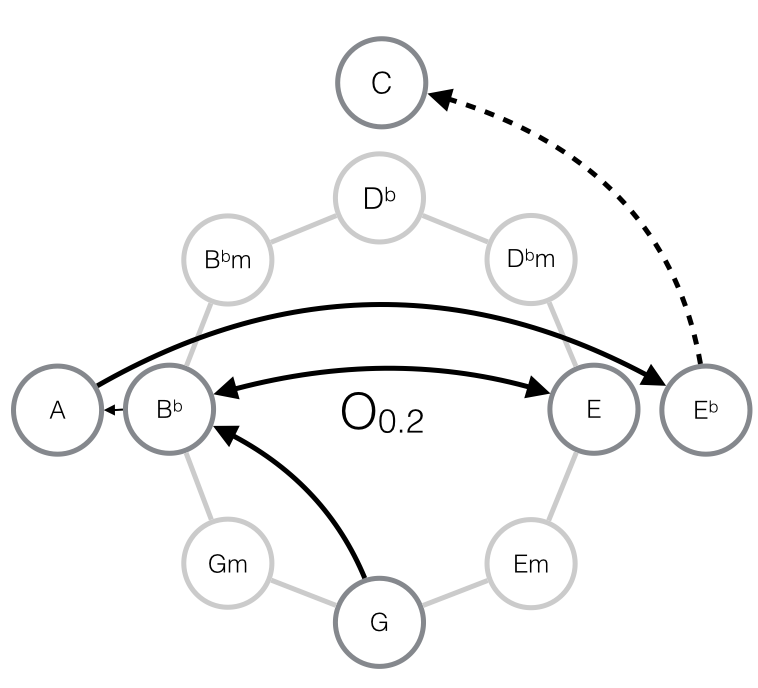
\includegraphics[width=0.8\linewidth]{STTMP_Leaving_Drydock_B}
	\caption{ST:TMP: Leaving Drydock B}
	\label{STTMP_Leaving_Drydock_B}
	\setfloatalignment{b}
\end{figure}
When preparing to exit from the interior to exterior shot, Goldsmith uses a \ac{MTTP} to advance (\textbf{m.23}). When we see the outer hull of Enterprise, Goldsmith uses his Star Trek theme, and does so throughout the score with various treatments. Figure \ref{STTMP_Leaving_Drydock_B} sees \textbf{m.28-30}. It is a three-part trumpet, brassy and pompous, but does not match any significant event on the screen. The harmonic movement however is interesting. Goldsmith moves in minor thirds right up to A, where he makes \textit{chromatic network modulation}. What follows is the Star Trek theme in 3:2 until we cut to the bridge again.

%-----------------------------------------------------------------------------
% D
%-----------------------------------------------------------------------------
\begin{figure}[h!]
\center
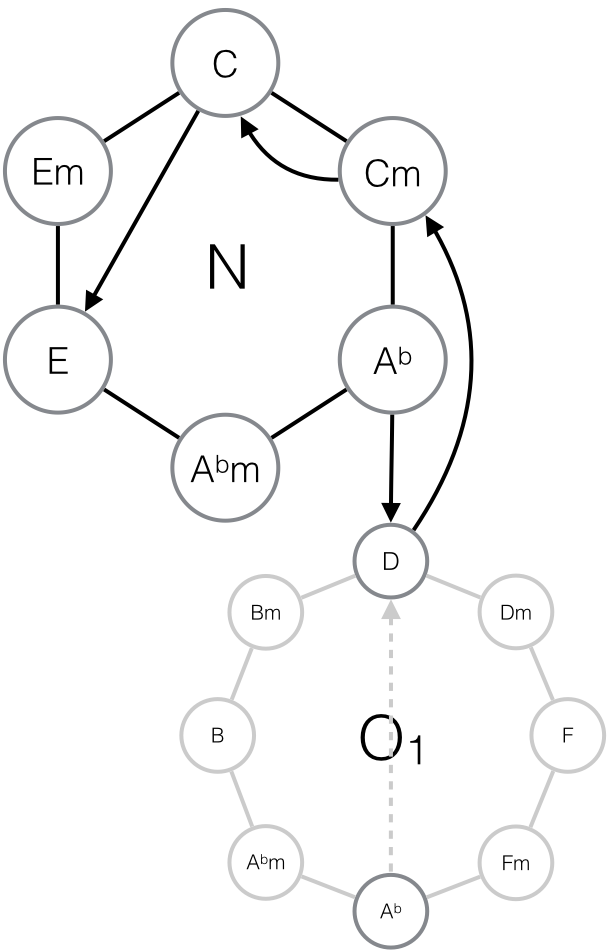
\includegraphics[width=0.6\linewidth]{STTMP_Leaving_Drydock_D}
	\caption{ST:TMP: Leaving Drydock D}
	\label{STTMP_Leaving_Drydock_D}
	\setfloatalignment{b}
\end{figure}
The restless ostinato mimics Kirk, who is clearly electric: ''Thrusters ahead, Mr. Sulu.'' The music builds and the harmonic progression (figure \ref{STTMP_Leaving_Drydock_D}) is as anxious as the captain. This time, the \ac{MTTP} is slightly softened with the incursion of G/B just before \bflat. We once again see the Enterprise, now leaving the drydock, followed by the full version of the Star Trek theme. 

At \textbf{m.72} we are back at the Enterprise, now down in engineering. The restless theme is back, mirroring the people working excitedly. With a new \ac{MTTP} we are out in space again, viewing the Enterprise slowly flying with Earth and the sun as a magnificent backdrop.
%-----------------------------------------------------------------------------
% J
%-----------------------------------------------------------------------------
With a small meter change, \lilyTimeSignature{3}{8}, we follow up from last shot down in engineering, figure \ref{STTMP_Leaving_Drydock_J}. Concealed inside the chord progression is the whole tone scale, \textit{pc} [0,2,4,6,8,t],\footnote{\keyboard{one=C,two=D,three=E,four=Fiss,five=Giss,six=Aiss,}} figure \ref{STTMP_Leaving_Drydock_J2}, creating a sense of wonder. The progression follows in figure \ref{STTMP_Leaving_Drydock_J}. Goldsmith works through major thirds, connecting them with a minor third, passing on with a \textbf{SLIDE} and continuing with chords with roots that follow minor thirds until \textbf{m.95} where he prepares a \ac{MTTP}, getting there through the two common tones \fiss and \aiss connecting \(D\flatx^{dim}\) and \fiss. After a small 3:2, mixolydian progression reminiscent of the Star Trek theme, we head back out to the Enterprise, now burning her engines to the Star Trek theme \textbf{m.99-103}.

\begin{figure*}
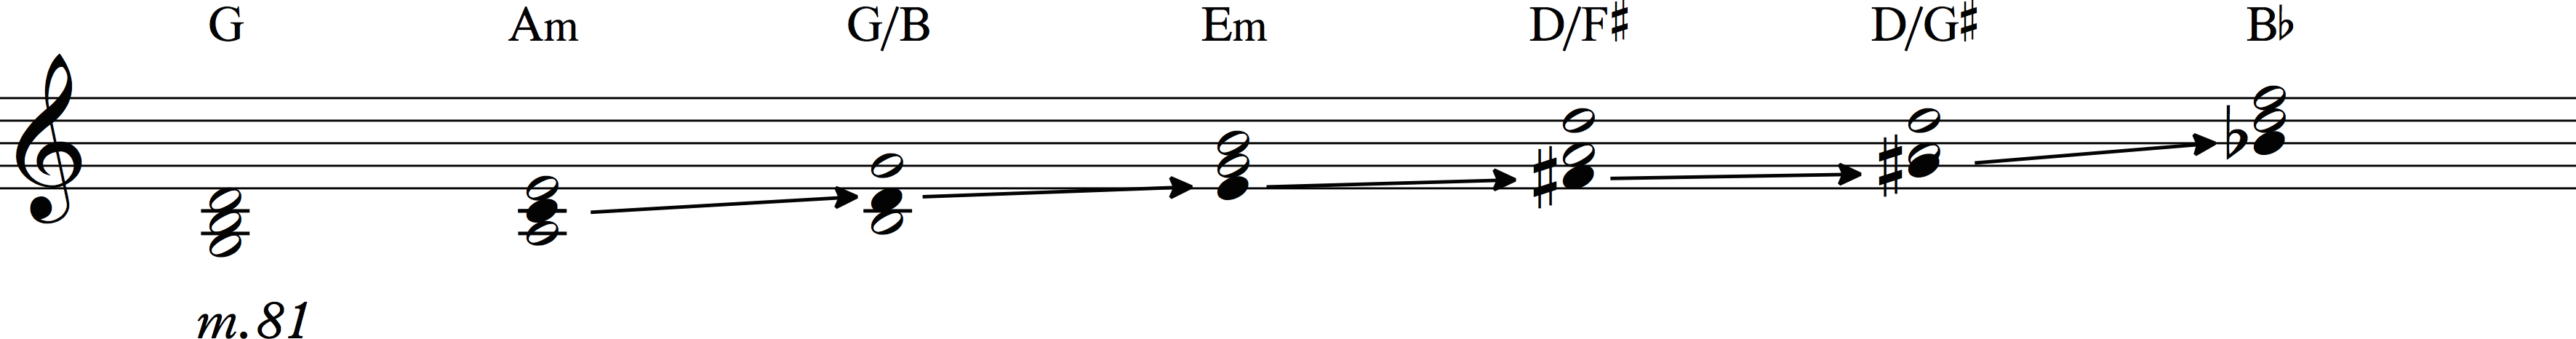
\includegraphics[width=\linewidth]{STTMP_Leaving_Drydock_J2}
	\caption{ST:TMP: Leaving Drydock J: Whole Tone Scale}
	\label{STTMP_Leaving_Drydock_J2}
	\setfloatalignment{b}
\end{figure*}

\begin{marginfigure}
\center
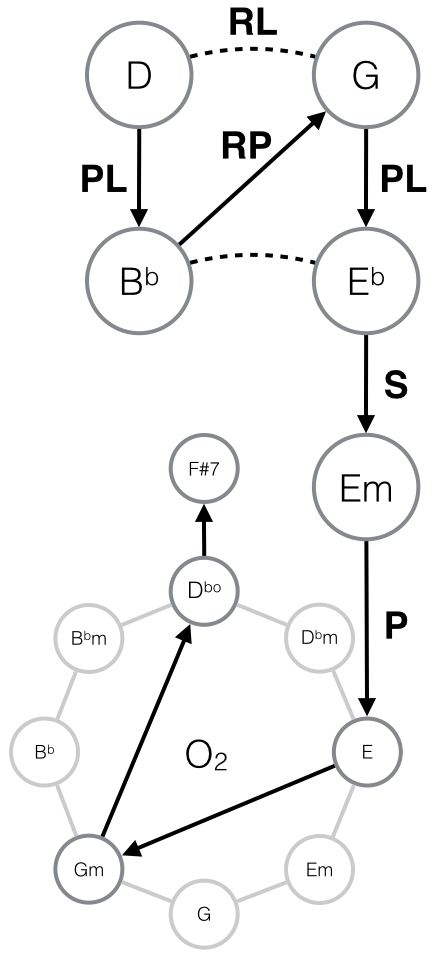
\includegraphics[width=\linewidth]{STTMP_Leaving_Drydock_J}
	\caption{ST:TMP: Leaving Drydock J}
	\label{STTMP_Leaving_Drydock_J}
	%\setfloatalignment{b}
\end{marginfigure}


%-----------------------------------------------------------------------------
% M
%-----------------------------------------------------------------------------
Back inside, the restless theme is repeated once more, continuing the third-progressions, figure \ref{STTMP_Leaving_Drydock_M}. At \textbf{m.111} the captain requests ''Viewer ahead.'' and we get a glimpse of the stars as they pass the ship. Kirk looks outwards proudly while the Star Trek theme plays 3:2. We cut to the outside and the theme returns to its original form as we see the Enterprise rockets past Venus.

\begin{figure}
\center
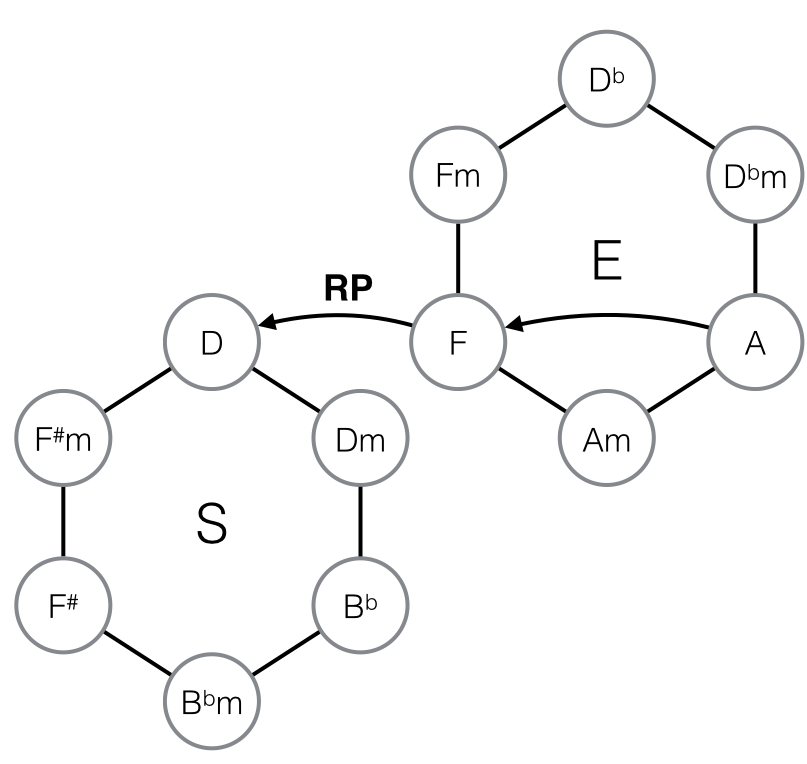
\includegraphics[width=0.8\linewidth]{STTMP_Leaving_Drydock_M}
	\caption{ST:TMP: Leaving Drydock M}
	\label{STTMP_Leaving_Drydock_M}
	\setfloatalignment{b}
\end{figure}


%-----------------------------------------------------------------------------
% PDF
%-----------------------------------------------------------------------------
\clearpage
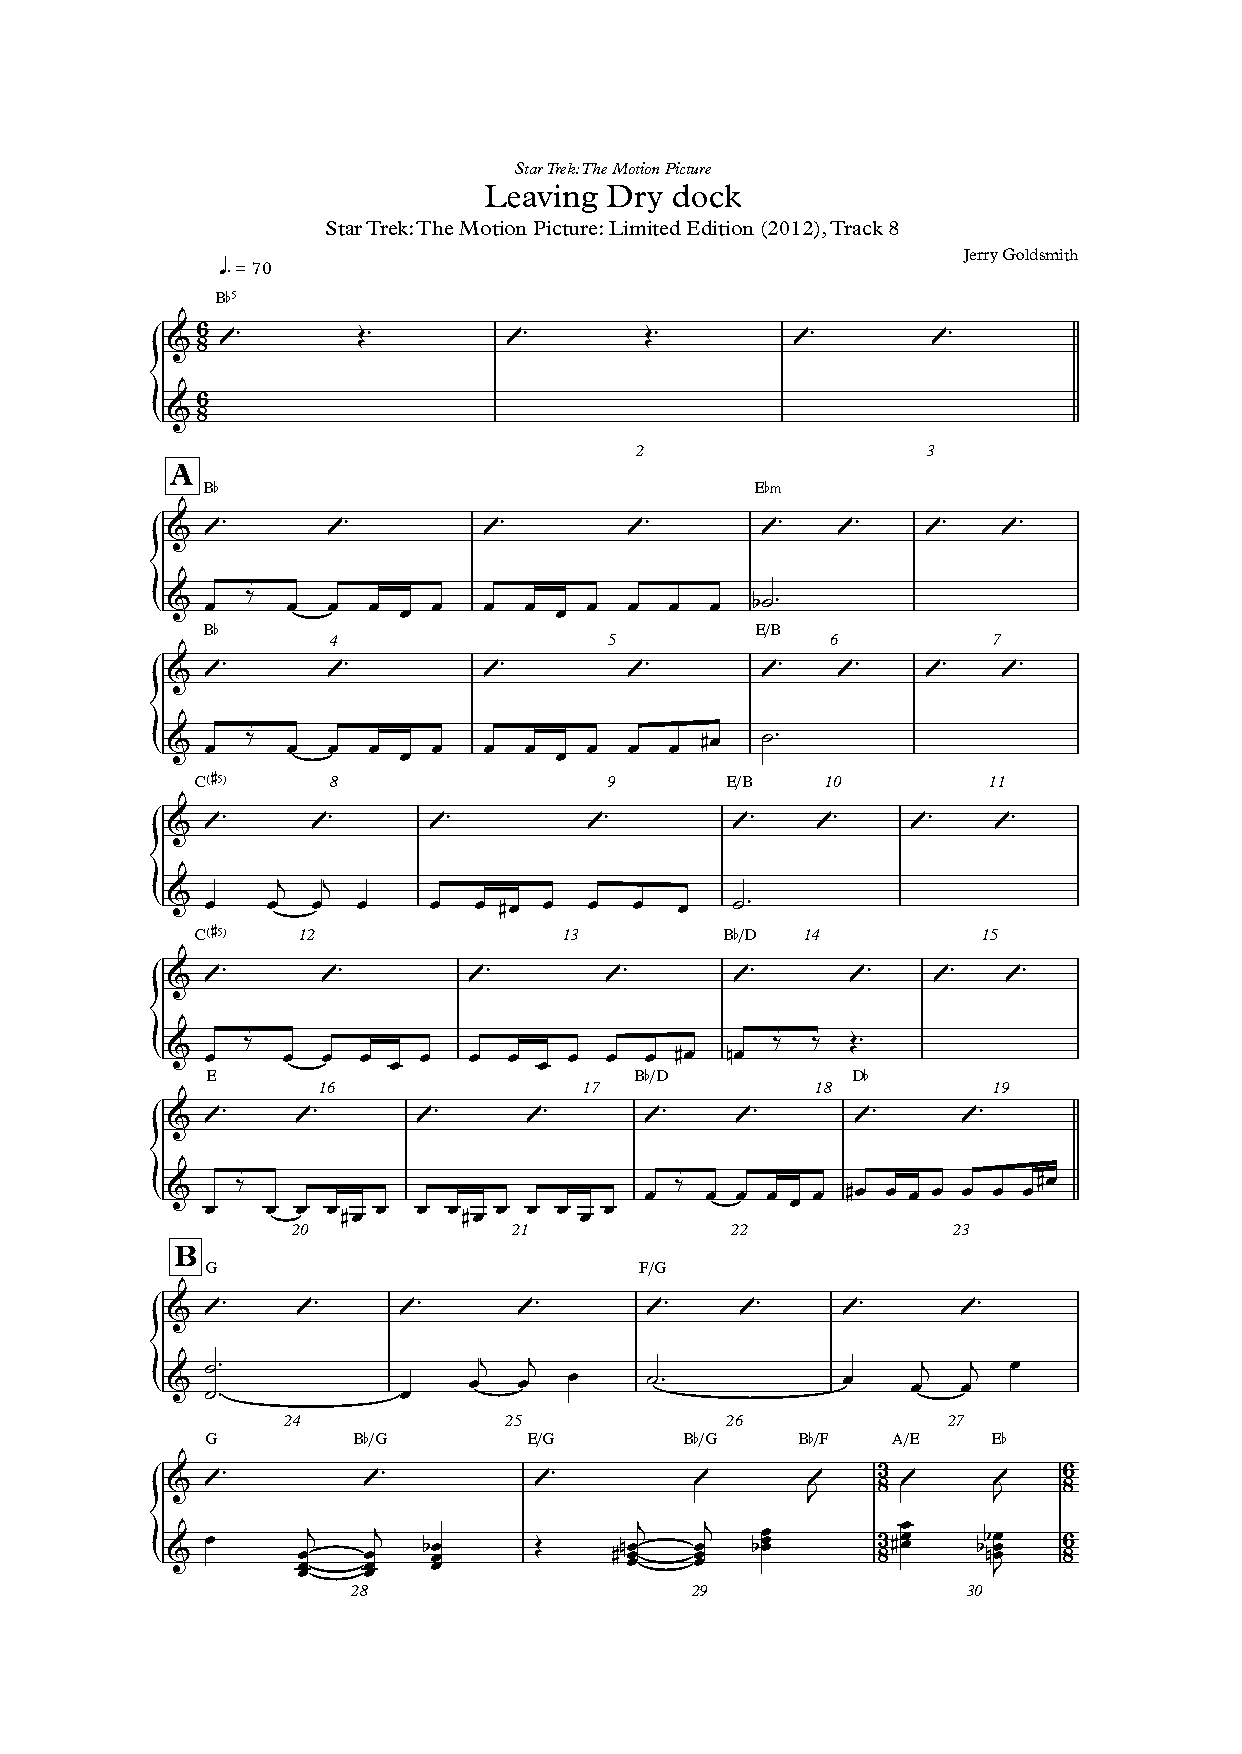
\includepdf[pages=-,pagecommand=\thispagestyle{fancy}]{pdf/st1/STTMP_Leaving_Drydock.pdf}

% Reviewed

% !TEX root = ../../../Masterthesis.tex

\chapter{Star Trek II: The Wrath of Khan}

\section{Main Title}\label{sec:st 2 main title}
%-----------------------------------------------------------------------------
% Introduction
%-----------------------------------------------------------------------------
\begin{figure}[h!]
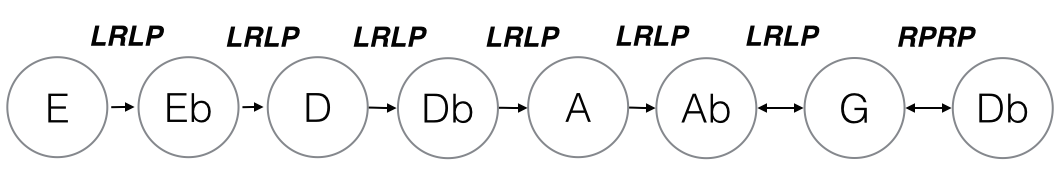
\includegraphics[width=\linewidth]{ST2_main_title_intro}
	\caption{ST 2: Main Title Introduction}
	\label{ST2_main_title_intro}
	\setfloatalignment{b}
\end{figure}
\noindent\newthought{A synth provides} a slowly evolving mysterious pad while the logos pass the screen. Soon after, we are traveling slowly through space and the trumpets play the Star Trek theme sequenced chromatically, figure \ref{ST2_main_title_intro}, from E downward to \eflat. The horns start playing a fiery sextuplet pattern in D doing a sort of call-and-response with the trumpets, sequencing downwards chromatically one more step to \dflat. Horner now repeats the sextuplet theme once more, but does a mediant modulation to A; the combined melodies create a whole tone feeling [1,3,5,9,E]\footnote{\keyboard{one=Ciss,two=Diss,three=F,four=A,five=B,}}. On m.12, the Star Trek Logo is seen moving into screen and it conforms to the screen by m.13. The tonal center in \textbf{m.}11-12 is G, flanked by a predominant chord substitute, \aflat and a \acf{MTTP} to \dflat.



%-----------------------------------------------------------------------------
% A
%-----------------------------------------------------------------------------
\begin{figure}[h!]
\center
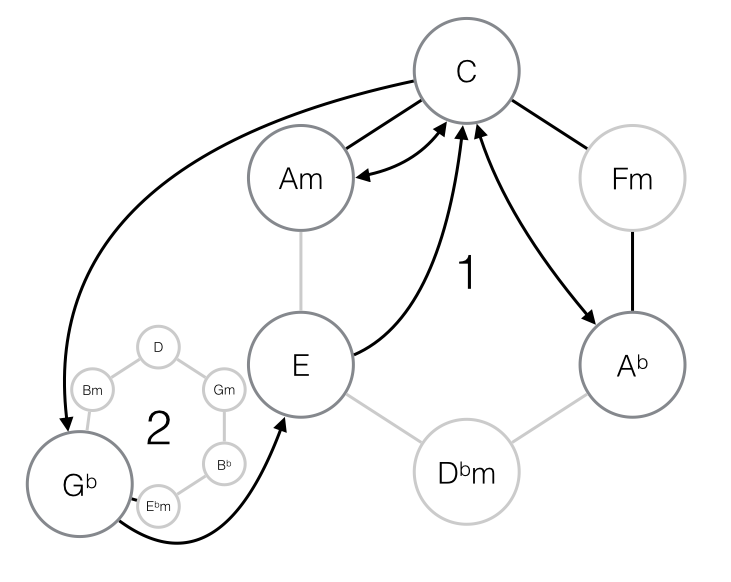
\includegraphics[width=0.7\linewidth]{ST2_main_title_a_pass_1}
	\caption{ST 2: Main Title A, pass 1}
	\label{ST2_main_title_a_pass_1}
	\setfloatalignment{b}
\end{figure}

The main theme is fanfare in C, figure \ref{ST2_main_title_a_pass_1}, but as one might expect from James Horner, the tonality is based on different circle then that of fifths. Instead of maneuvering in \textbf{NR\(_{1}\)}, he makes a short detour to \textbf{NR\(_{2}\)} to fetch \gflat. The melody uses the fifth mode of the melodic minor scale, i.e. the so called mixolydian \(\flatx{6}\) [0,2,4,5,7,8,T]\footnote{\keyboard{one=C,two=D,three=E,four=F,five=G,six=Giss,seven=Aiss,}}. A duality might be assumed by the fact that both Ionian, with the occurrence of [9], and melodic minor [8,10] is explored within the same phrase. 

\begin{figure}[h!]
\center
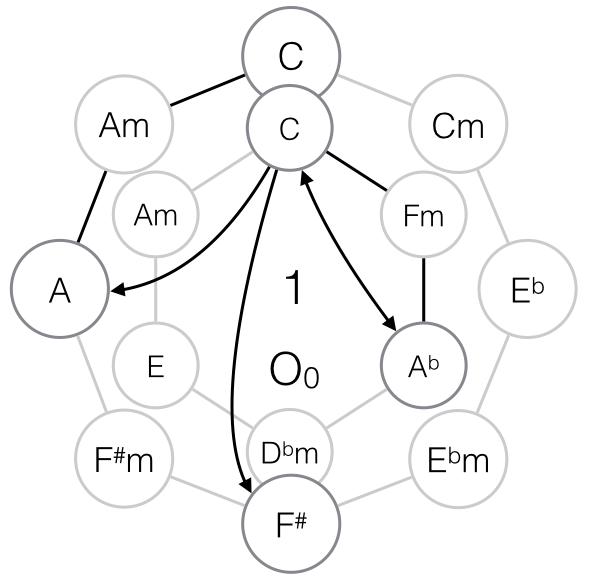
\includegraphics[width=0.7\linewidth]{ST2_main_title_a_pass_2}
	\caption{ST 2: Main Title A, pass 2}
	\label{ST2_main_title_a_pass_2}
	\setfloatalignment{b}
\end{figure}

The second pass, figure \ref{ST2_main_title_a_pass_2} holds the same harmonic idea but uses A instead of Am, making the progression almost completely Octatonic\footnote{Much like we find in Goldsmith's harmonic language.}. 

%-----------------------------------------------------------------------------
% B and C
%-----------------------------------------------------------------------------
\begin{figure}[h!]
\center
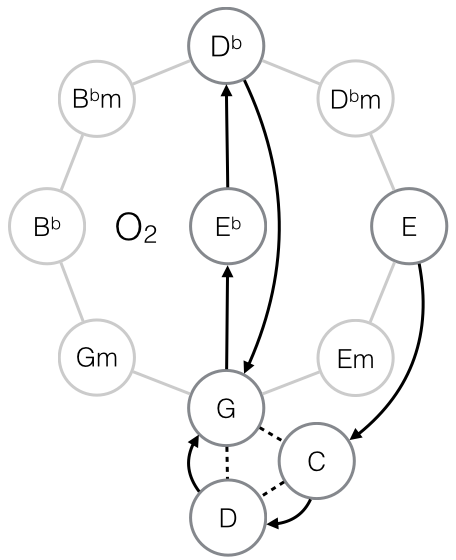
\includegraphics[width=0.7\linewidth]{ST2_main_title_b}
	\caption{ST 2: Main Title B}
	\label{ST2_main_title_b}
	\setfloatalignment{b}
\end{figure}

B starts with a triplet ostinato over E(\(\sharpx 5\)), played by the cellos, figure \ref{ST2_main_title_b}. The sense of Cartesian dualism intensifies with the continued mixolydian \(\flatx{6}\), cross combining major and minor. Harmonically the difference between A and B is enough to distinguish them, but the melody plays a variation on the main theme making the whole section somewhat familiar, yet distant to its origin. On bar 4 m.26, Horner starts a cascading flurry of chords, seemingly unrelated, but seen through \ac{nRT}, there is a clear idea driving the progression. From E, Horner makes a plagal cadence \(IV-V\) to G before moving through \(\flatx{VI}-\sharpx{IVb}\), making the bass line reminiscent of an Aeolian Cadence \(\flatx{VI}-\flatx{VII}-I\). m.32 lands on G while the melody is working a chromatically altered octatonic scale. 

%-----------------------------------------------------------------------------
% A and B'
%-----------------------------------------------------------------------------
\begin{figure}[h!]
\center
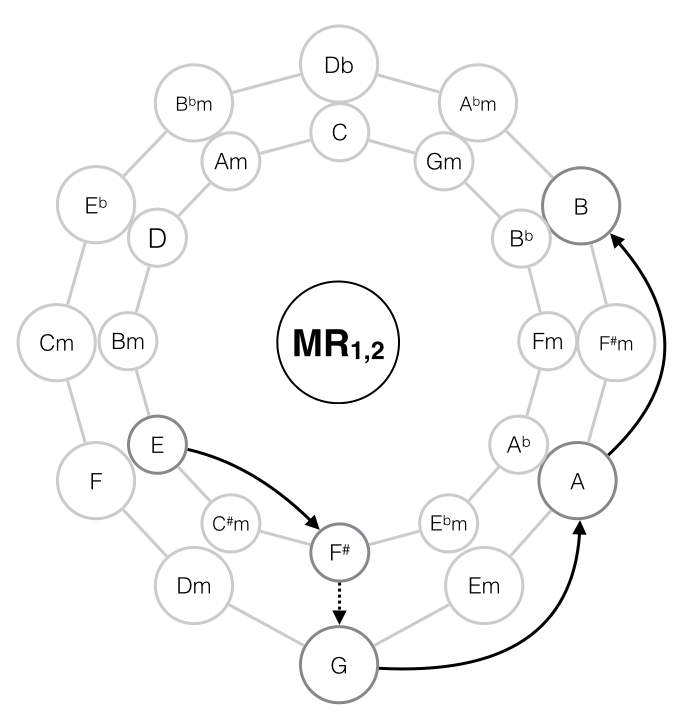
\includegraphics[width=0.7\linewidth]{ST2_main_title_b'}
	\caption{ST 2: Main Title B'}
	\label{ST2_main_title_b'}
	\setfloatalignment{b}
\end{figure}
After a reprise of A, a longer variation of B is developed, beginning at m.40, figure \ref{ST2_main_title_b'}. This time the low strings are playing melody while the high strings are playing the virtuositic sextuplet ostinato. This is the same ostinato that earlier was played as an arpeggiated \chord{E}{aug}, only double time. The harmonic backdrop moves through the \textbf{MR} circles, making a network modulation when jumping from \fiss to G. The melody follows the harmonic structure until m.48 where it follows the phrygian dominant scale [0,1,4,5,7,8,T]. The part repeats with the melody  played by the high strings, ever so slightly altered, and the ostinato returns to the previous pattern.

%-----------------------------------------------------------------------------
% Ending
%-----------------------------------------------------------------------------
The ending introduces itself in m.56, figure \ref{ST2_main_title_ending}, where Courage's Star Trek theme rings in with a lone trumpet. All the while, the strings play the same  phrygian dominant scale as a counterpoint, landing on B. From there the fanfare theme is used, sequencing ever upwards. If one were to see the final C as Tonic, the progression would follow: \(III-(MTTP)-\flatx{VII}-(Mediant)-II-\flatx{II}-(tritone substitute)-I\), making it a heavily distorted \(iii-vi-ii-V-I\). 

\clearpage
\begin{figure}
\center
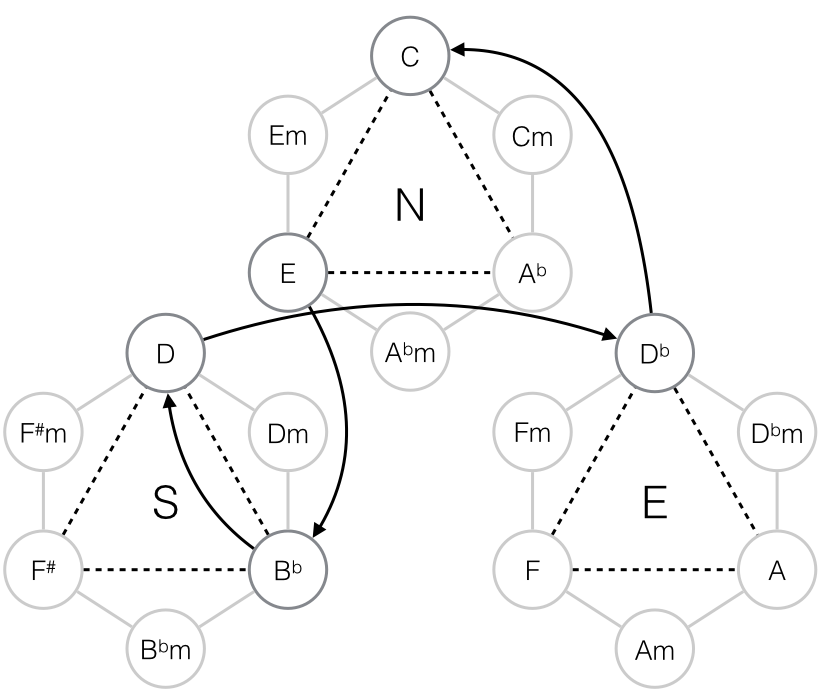
\includegraphics[width=\linewidth]{ST2_main_title_ending}
	\caption{ST 2: Main Title Ending}
	\label{ST2_main_title_ending}
	%\setfloatalignment{b}
\end{figure}



%-----------------------------------------------------------------------------
% PDF
%-----------------------------------------------------------------------------
\clearpage
\includepdf[pages=-,pagecommand=\thispagestyle{fancy}]{pdf/ST2/ST2_Main_Title}

% Reviewed
% !TEX root = ../../../Masterthesis.tex
\section{Enterprise Clears Moorings}
\begin{figure}[h!]
\center
\includegraphics[width=0.6\linewidth]{ST2_Enterprise_PL}
	\caption{ST 2: Enterprise Clears Moorings, PL network}
	\label{ST2_Enterprise_PL}
	\setfloatalignment{b}
\end{figure}

\noindent The cue starts with an exterior shot of the Enterprise. Horner introduces a lydian inspired, slow and majestic theme as the Enterprise lights her external light buoys, preparing to leave the space dock. 

As soon as Kirk and Dr. McCoy enters the bridge, military snare drums and Horner's Star Trek theme plays over a G pedal. Woodwinds and wind chimes provide some lydian glitter just as the theme plays again. Spock is the Captain of the Enterprise and is seen overseeing the final preparations. The theme relies heavily on the mixolydian \flat6 scale\footnote{\keyboard{one=C,two=D,three=E,four=F,five=G,six=Giss,seven=Aiss,}\\Mixolydian \flat6: \textit{pc} [0,2,4,5,7,8,T]} and with it provides the harmonic backdrop.

\textbf{m.18-19} provides a section of \textit{parallel harmonic displacement}\footnote{Not unlike what we find in jazz big band traditions, where they are known as \textit{block chords} or \textit{chorale style harmony}.} seemingly unprovoked. It might be a mimicking of Spock, the half human and half Vulcan who is famous for his logic and lack of emotion; though this is pure speculation. In any case, it works as a transition and modulation for the Star Trek theme, now in F, and with an F pedal point until \textbf{m.29}.  

Figure \ref{ST2_Enterprise_PL} is a overview of the way Horner uses major thirds as a harmonic roadmap and has been the rule until now. Spock asks Lt. Saavik if she has ever before piloted a starship from the space dock. As she replies, Horner switches to a wondrous feeling \acf{MTTP} and hence makes use of his other harmonic road map, the RPRP network, as seen in figure \ref{ST2_Enterprise_RPRP}.

\begin{figure}
\center
\includegraphics[width=0.6\linewidth]{ST2_Enterprise_RPRP}
	\caption{ST 2: Enterprise Clears Moorings, RPRP network}
	\label{ST2_Enterprise_RPRP}
	\setfloatalignment{b}
\end{figure}

Lt. Saavik accepts the challenge, which is followed by the main theme, and walks to the captain's chair. When walking Horner introduces a theme in A (\textbf{m.29}) which is lydian and familiar in tonality just as the theme in the beginning of the cue; however, this is not a theme but more for providing a sense of wonderment. 

Kirk is obviously nervous as Spock orders Lt. Saavik to take the ship out. The Star Trek theme modulates to D and sounds one last time before an accelerando and crescendo raises the excitement, along with Kirk, and hits the point of the Enterprise departing. Horner uses a variation of the sextuplet theme used in the Main Titles. The flurry of notes is backed up by a rising G lydian scale in the lower brass. After another \textbf{RPRP}, Horner revisits the Main Titles more, or less, exactly. From letter \textbf{I}, Horner has displaced the melody by one beat per what he did during the Main Titles. The chord structure Horner uses are major chords over the E minor scale (figure \ref{ST2_Enterprise_eminor}).

\begin{marginfigure}
%\center
\includegraphics[width=\linewidth]{ST2_Enterprise_eminor}
	\caption{ST 2: Enterprise Clears Moorings, Major Chords over the E Minor Scale}
	\label{ST2_Enterprise_eminor}
	\setfloatalignment{b}
\end{marginfigure}

From \textbf{m.67} we return to the bridge and the music turns ominous. Descending and arpeggiated \(B^{(\sharp5)}\)'s with a quite energetic \(\hat{3}\) as the root. As with Spock, this seems unmotivated until one considers that working on a spaceship can be quite hazardous. The same descending pattern modulates up a fourth and is now joined by a fanfare that builds until Enterprise enters warp speed where Horner's music does exactly the same. There is a tiny tail where a major sixth is repeated, but the film cuts to a shot of a dark space station and the music turns to a flat 6, perhaps, making a prediction on its future.

%-----------------------------------------------------------------------------
% PDF
%-----------------------------------------------------------------------------
\clearpage
\includepdf[pages=-,pagecommand=\thispagestyle{fancy}]{pdf/st2/ST2_Enterprise_Clears_Moorings.pdf}

% Reviewed

% !TEX root = ../../../Masterthesis.tex

\chapter{Star Trek VIII: First Contact}\label{ch:st 8}

\section{Main Title}
%-----------------------------------------------------------------------------
% Introduction, A and B
%-----------------------------------------------------------------------------
\begin{figure}[h!]
\center
\includegraphics[width=0.7\linewidth]{ST8_introduction}
	\caption{ST 8: Introduction}
	\label{ST8_introduction}
	\setfloatalignment{b}
\end{figure}

\noindent\newthought{In direct opposition} to the tone of the movie, the main title of Star Trek: First Contact provides an emotionally charged and inspiring tone. The introduction, figure \ref{ST8_introduction}, treats us with the Star Trek theme twice, first in D-A and then in \fiss-\ciss, quickly moving down through \bflatm to F, which one might describe as a plagal cadence with minor subdominant. The tonal energy in A and B is very much centered around the well established \(I-IV-V\) and \(vi-IV-ii-V-I\) cycles. 
%-----------------------------------------------------------------------------
% C
%-----------------------------------------------------------------------------
From m. 28 Goldsmith executes a modulation to the dominant C and repeats \(ii-V\) twice before moving to Cm. He then executes a Aeolian Cadence, figure \ref{ST8_aeolian_cadence}, modulating to F major and ending on the dominant C in m.35. The main theme of the cue repeats once more ending with a lydian, ``fantastical'' sounding progression. 
\begin{marginfigure}
\includegraphics[width=\linewidth]{ST8_aeolian_cadence}
	\caption{Aeolian Cadence}
	\label{ST8_aeolian_cadence}
	%\setfloatalignment{b}
\end{marginfigure}

%-----------------------------------------------------------------------------
% PDF
%-----------------------------------------------------------------------------
\clearpage
\includepdf[pages=-,pagecommand=\thispagestyle{fancy}]{pdf/ST8/ST08_First_Contact_Main_Title.pdf}

% Reviewed
% !TEX root = ../../../Masterthesis.tex
\section{Red Alert}
%-----------------------------------------------------------------------------
% A
%-----------------------------------------------------------------------------
\begin{figure*}[h!]
\center
\includegraphics[width=\linewidth]{ST8_schenker_A}
	\caption{ST 8: Red Alert A: Prolonged Aeolian Cadence.}
	\label{ST8_schenker_A}
	%\setfloatalignment{b}
\end{figure*}

\noindent Picard and the crew onboard the Enterprise have just witnessed, by way of audio, the beginning of the Borg attack on earth. Picard is helpless, being several lightyears away. Determined to do something, Picard orders his crew to prepare to enter warp speed toward earth. The main theme of the film plays while Picard orders "all hands" to battle stations. As soon as we see the Enterprise, the Star Trek theme is played, making a quick \ac{MTTP} to \ciss before landing on m.8: Cm.

%-----------------------------------------------------------------------------
% Klingon
%-----------------------------------------------------------------------------
\begin{figure}[h!]
\center
\includegraphics[width=0.7\linewidth]{ST8_red_alert_D}
	\caption{ST 8: Red Alert Klingon}
	\label{ST8_red_alert_D}
	\setfloatalignment{b}
\end{figure}

The Borg theme plays while a single Borg ship is seen fighting a number of ships from Starfleet. The battle is not unfolding in Starfleet's favor. We enter the bridge of a badly damaged ship, the USS Defiant. The crew are either dead or heavily injured. All of the sudden, the Klingon theme\footnote{written by Jerry Goldsmith for \ac{ST:TMP}.} is heard and we see Worf as he exclaims: ``Perhaps today \textit{is} a good day to die! Prepare for ramming speed!'' At that very moment, the Enterprise arrives at the battleground and intervenes, shielding the Defiant from the Borg. The music keeps Mickey-mousing, as it were, with the Star Trek theme, which is now playing to signify the presence of USS Enterprise. The theme is played twice and makes a \acf{MTTP} from \aflat to D (figure \ref{ST8_red_alert_D}).

The scene cuts to the bridge of the Enterprise and the music plays a variant of the Borg theme, m.30. The military snare drum accompanies this part, building more tension as Picard prepares and organizes the rest of the fleet for a joint strike at the Borg ship.
%-----------------------------------------------------------------------------
% Ending
%-----------------------------------------------------------------------------
As the tension in the scene builds, the music retains the tension by applying a D pedal bass throughout a series of major chords which have their foundation in the octatonic scale. This builds till part \textbf{H}, where the modified Borg theme plays, heard in m.33-39, figure \ref{ST8_red_alert_G}.

\begin{figure}
\center
\includegraphics[width=0.5\linewidth]{ST8_red_alert_G}
	\caption{ST 8: Red Alert Ending}
	\label{ST8_red_alert_G}
	%\setfloatalignment{b}
\end{figure}


%-----------------------------------------------------------------------------
% PDF
%-----------------------------------------------------------------------------
\clearpage
\includepdf[pages=-,pagecommand=\thispagestyle{fancy}]{pdf/st8/ST8_Red_Alert.pdf}

% Reviewed

% !TEX root = ../../../Masterthesis.tex

\chapter{Star Trek X: Nemesis}

\section{Remus (Main Title)}\label{sec:st 10}
%-----------------------------------------------------------------------------
% Introduction
%-----------------------------------------------------------------------------
\begin{figure}
\center
\includegraphics[width=0.5\linewidth]{ST10_main_title_intro_1}
	\caption{ST 10: Main Title Intro 1}
	\label{ST10_main_title_intro_1}
	\setfloatalignment{b}
\end{figure}

\noindent\newthought{The music begins} with the introduction of the Paramount logo. This time there is a synth and string pad slowly evolving through \(\hat{5}-\hat{1}-\hat{5}\) ending on a piercing, sweeping, high-pitch pad over D\(^{\triangle 7}\) (figure \ref{ST10_main_title_intro_1}). This fades down fairly quickly to a D\(^{5}\), which provides the harmonic bed for the melody. The melody starts by ascending two M3's, resting on the fifth, creating an uneasy feeling. The melody uses the fifth mode of melodic minor\footnote{Mixolydian\(\flatx{6}\)=[0,2,4,5,7,8,T]} giving both minor \(iv\) and \(v\). 

%-----------------------------------------------------------------------------
% Introduction part 2
%-----------------------------------------------------------------------------
\begin{figure}
\center
\includegraphics[width=0.5\linewidth]{ST10_main_title_intro_2}
	\caption{ST 10: Main Title Intro 2}
	\label{ST10_main_title_intro_2}
	\setfloatalignment{b}
\end{figure}
In m.10, the famous ``Courage" Theme comes to life as the Star Trek tittle hits the screen. It modulates and repeats as the subtitle ``Nemesis'' is revealed. The modulation makes a coupling through the \(\hat{3}\) of A, making it the new \(\hat{5}\) of \fiss (figure \ref{ST10_main_title_intro_2}).

%-----------------------------------------------------------------------------
% A
%-----------------------------------------------------------------------------
\begin{figure}
\center
\includegraphics[width=0.5\linewidth]{ST10_main_title_A}
	\caption{ST 10: Main Title A}
	\label{ST10_main_title_A}
	\setfloatalignment{b}
\end{figure}
After a short percussive pattern with military snare drums and timpani, the main theme plays. This happens while we fly toward a number of planets, traveling all the way down to an alien city. Supporting the melody is percussion and a metallic synth, providing an ominous military feeling.The scale is pure minor and the chords alternate between \(vi(I)-IV\) (figure \ref{ST10_main_title_A}).

%-----------------------------------------------------------------------------
% B
%-----------------------------------------------------------------------------
As soon as the dialogue starts, the music drops down and an eerie melody plays. The sonority perceived is that of chords built upon [048]'s, thanks to the same Mixolydian\(\flatx{6}\) used in the introduction. 

%-----------------------------------------------------------------------------
% PDF
%-----------------------------------------------------------------------------
\clearpage
\includepdf[pages=-,pagecommand=\thispagestyle{fancy}]{pdf/ST10/ST10_Remus.pdf}

% Reviewed
% !TEX root = ../../../Masterthesis.tex
\section{Attack Pattern}\label{sec:attack pattern}
%-----------------------------------------------------------------------------
% Part ABC
%-----------------------------------------------------------------------------
\begin{figure}[h!]
\center
\includegraphics[width=0.5\linewidth]{ST10_attack_pattern_abce}
	\caption{ST 10: Attack Pattern, part A, B, C and E}
	\label{ST10_attack_pattern_abce}
	\setfloatalignment{b}
\end{figure}
\noindent Captain Picard and Lt. Cdr. Data are conversing in the cartography room when they realize they are going to lose long range communications. The music starts at the moment of realization. It is a tension-building, syncopated motif in \lilyTimeSignature{7}{4} played by the low strings (figure \ref{ST10_attack_pattern_abce}). A sweeping synth and horns play the second motif as both Data and Picard realize that this is the moment Shinzon has been waiting for. Picard orders evasive maneuvers, but Shinzon has already begun the attack. The tonality is exclusively octatonic\marginnote{\keyboard{C,Ciss,Diss,E,Fiss,G,A,Aiss}}, giving the overall sonority, combined with odd meters, an aggressive and uneasy nature. Enterprise is critically hit and loosing warp capabilities. Shinzon's ship is seen turning around to continue the attack. The musical meters adapt to mickey-mouse the cuts. 

The music drops in energy and a new motif enters, \textbf{C}, as we cut to the interior of Shinzon's ship where the attack on the Enterprise continues. Picard returns to the bridge and orders retaliation and the music picks up again. Shinzon's ship is cloaked and, ultimately, the Enterprise manages to inflict only minimal damage. 

The music, now at letter \textbf{C}, introduces a new motif, \textit{motif 3} accompanied by \textit{motif 1}. All in all, it is very subdued and clearly restrained, mirroring the screen as there is a momentary absence of fire. The crew of Enterprise gives rapports on current status. 

\begin{marginfigure}
%\center
\includegraphics[width=\linewidth]{ST10_attack_pattern_D}
	\caption{ST 10: Attack Pattern, part D and E}
	\label{ST10_attack_pattern_D}
	%\setfloatalignment{b}
\end{marginfigure}

Shinzon plans his ferocious attack, and Goldsmith does the first, and only network modulation, to Cm (figure \ref{ST10_attack_pattern_D}). From letter \textbf{E} the planning evolves, and letter \textbf{F} is introduced simultaneously as the attack explodes into action. The battle ends when the Enterprise can take no more; Shinzon hails Picard and the battle ends. 
%-----------------------------------------------------------------------------
% PDF
%-----------------------------------------------------------------------------
\clearpage
\includepdf[pages=-,pagecommand=\thispagestyle{fancy}]{pdf/st10/ST10_Attack_Pattern} 

% Reviewed

% !TEX root = ../../../Masterthesis.tex

\chapter{Star Trek XI: Star Trek}\label{ch:st 11}

\section{Star Trek}

\begin{figure}[h!]
\center
\includegraphics[width=0.7\linewidth]{ST11_star_trek_1}
	\caption{ST 11: Star Trek}
	\label{ST11_star_trek_1}
	%\setfloatalignment{b}
\end{figure}

\begin{marginfigure}
%\center
\includegraphics[width=\linewidth]{ST11_star_trek_1_1}
	\caption{ST 11: Star Trek: Transformational Cycle}
	\label{ST11_star_trek_1_1}
	%\setfloatalignment{b}
\end{marginfigure}

\noindent\newthought{Not unlike the} rest of the Star Trek franchise, Star Trek XI begins with a short overture, presenting the main tonality and mood of the coming score. The cue is quite clearly constructed in the circle of fifths, but honoring the ``space progression'' \ac{MTTP}. The progression mapped out in Dm follows: \(i-\flatx{VI}-\flatx{II}-V\). The sonority is soft but curious, with pads and soft strings supporting the melody. The melody is built upon a simple motif that transforms with the harmony.

With the main theme presented, Giacchino presents the second main theme used throughout\footnote{\includegraphics[width=\linewidth]{ST11_motif}}. 
%-----------------------------------------------------------------------------
% PDF
%-----------------------------------------------------------------------------
\clearpage
\includepdf[pages=-,pagecommand=\thispagestyle{fancy}]{pdf/ST11/ST_11_1_Star_Trek.pdf}

% Reviewed
% !TEX root = ../../../Masterthesis.tex
\section{Main Title}
\begin{figure}[h!]
\center
\includegraphics[width=\linewidth]{ST11_main_title}
	\caption{ST 11: Main Title}
	\label{ST_11_main_title}
	\setfloatalignment{b}
\end{figure}
After the action packed encounter with the time traveling Romulans has subsided, the wife of Kirk Senior gives birth to James T. Kirk. The  rhythmical motif of Star Trek begins playing while a fluttering flute plays a melody based upon harmonic minor. In essence, this cue is the same as the first. The motifs are the same with the exception of their order; first comes the rhythmical motif, then the main theme is re-harmonized slightly with \(i-v\) instead of \(i-\flat{VI}\) and, instead of triplets, the theme is stretched out to quarter-notes. 

%-----------------------------------------------------------------------------
% PDF
%-----------------------------------------------------------------------------
\clearpage
\includepdf[pages=-,pagecommand=\thispagestyle{fancy}]{pdf/ST11/ST_11_2_Main_Title.pdf}

% Reviewed

% !TEX root = ../../../Masterthesis.tex
\section{Hangar Management}
\begin{marginfigure}
\center
\includegraphics[width=0.6\linewidth]{ST_11_hangar_managment_1}
	\caption{ST 11: Hangar Management A}
	\label{ST_11_hangar_managment_1}
	%\setfloatalignment{b}
\end{marginfigure}
The scene begins after Kirk has been caught cheating on the ''Kobayashi Maru'' and he is now facing public reprimand. Admiral Barnett gets word that the Vulcan home-planet is under attack and he orders the cadets to report to Hanger One and await ship assignment. The scene shifts to the hanger where hundreds of people and shuttle crafts are preparing to leave. A variant on the new Giacchino Star Trek theme is heard in the french horns, accompanied by marching snare drums, staccato strings and tuned bass drums\footnote{The movie cue and the CD cue do differ; the movie features taikos to accent the beat whereas the CD track does not.}. The tonality is natural minor, \({iii}{\Leftrightarrow}{vi}\), centered around \aflat (figure \ref{ST_11_hangar_managment_1}). The Barracks Leader\footnote{Cameo by \textbf{Star Gate} fame ''Dr. Carson Beckett'': \textit{Paul McGillion}.} calls out the cadet assignments. When Kirk notices his name is not called, the music calms to a solo trumpet playing another variation of the new Star Trek theme--this time with a dorian feel. Kirk approaches the barracks leader and asks why his name was not called. The barracks leader informs Kirk that he is on academic suspension, meaning, he is grounded until the academy board's ruling. The music grinds to a halt while McCoy supports Kirk the best he can, but leaves to board the shuttle craft. The new Star Trek theme enters solemnly (figure \ref{ST_11_hangar_managment_2}) at m.12, signifying Kirk's standing, left behind and alone.

\begin{marginfigure}
\center
\includegraphics[width=\linewidth]{ST_11_hangar_managment_2}
	\caption{ST 11: Hangar Management B}
	\label{ST_11_hangar_managment_2}
	%\setfloatalignment{b}
\end{marginfigure}
 
\begin{marginfigure}
\center
\includegraphics[width=\linewidth]{ST_11_hangar_managment_3}
	\caption{ST 11: Hangar Management D}
	\label{ST_11_hangar_managment_3}
	%\setfloatalignment{b}
\end{marginfigure}
McCoy has a change of mind, however, and the music makes a metric modulation while McCoy doubles back to fetch Kirk: ''Come with me!'' We now focus on Uhura who is assigned to the USS Farragut. Obviously displeased by this, she storms passed Kirk and McCoy who are discussing: ''Bones, where are we going?'', ''You'll see!'' A few strides later she meets Spock, her superior officer, asking why she was not picked out for the USS Enterprise. The music turns sweeter (figure \ref{ST_11_hangar_managment_3}), with the oboe playing a melody with a slight touch of something tongue-in-cheek, perhaps portraying the ferocious femininity emitting from Uhura as she makes an inarguable case for herself. Spock tries to defend his decision by placing Uhura on the USS Farragut on the basis of ''avoiding the appearance of favoritism.''. This does not go down well with Uhura who simply states: ''No. I'm assigned to the Enterprise.''. Spock swiftly and wisely makes an adjustment in the rosters to confirm.

''What are you doing?!'' Kirk asks. ''I'm doing you a favor.'' McCoy replies. The music is still calm, but the sonority has changed from dorian to lydian. This gives us the feeling that something wonderful and fantastic is going to happen. And indeed it does; McCoy injects Kirk with a vaccine for some aggressive disease causing Kirk to experience some severe allergic reactions. McCoy drags Kirk to a shuttle craft, and the musical figure modulates from \dflat to E, raising the energy levels (figure \ref{ST_11_hangar_managment_4}). But instead of a call-and-response, a trumpet now plays hints of the original Star Trek theme. McCoy then invokes protocol and rank to let Kirk join the shuttle craft. At the very end of the sequence, the original Star Trek theme is heard.

\begin{marginfigure}
\center
\includegraphics[width=0.7\linewidth]{ST_11_hangar_managment_4}
	\caption{ST 11: Hangar Management E}
	\label{ST_11_hangar_managment_4}
	%\setfloatalignment{b}
\end{marginfigure}

%-----------------------------------------------------------------------------
% PDF
%-----------------------------------------------------------------------------
\clearpage
\includepdf[pages=-,pagecommand=\thispagestyle{fancy}]{pdf/st11/ST_11_13_hangar_management}

% Reviewed

% !TEX root = ../../../Masterthesis.tex

\chapter{Star Trek XII: Into Darkness}\label{ch:into_darkness}

\section{Logos}\label{sec:st 12}
\newthought{The main title} in Star Trek: Into Darkness is, for all intents and purposes, identical to the ``Star Trek'' cue in Star Trek XI. What differs is the orchestration, which adds emphasis to the harp and adds the use of a choir.

%-----------------------------------------------------------------------------
% PDF
%-----------------------------------------------------------------------------
\clearpage
\includepdf[pages=-,pagecommand=\thispagestyle{fancy}]{pdf/ST12/ST12_Main_Title.pdf}

% Reviewed
% !TEX root = ../../../Masterthesis.tex

\section{London Falling}
This cue starts at approximately 0:16:34 right after Kirk's reprimand. A piano plays an arpeggiated \bflatm,(figure \ref{ST12_london_falling_motif_1}) while a solo oboe plays a simple theme: \textbf{theme B}. We see a birds eye view of London. The strings join the arpeggio, steadily intensifying when the main antagonist, Kahn, is using a medical device to extract his own blood into a vial. He places the tube in a container, along with a silver ring and all the while the music crescendos over the same \bflatm; all that changes is the thickness of the orchestration and the dynamic. 
\begin{marginfigure}
\includegraphics[width=\linewidth]{ST12_london_falling_motif_1}
	\caption{London Falling Motif 1}
	\label{ST12_london_falling_motif_1}
\end{marginfigure}

With \textit{subito piano}, the strings play very lightly in the top register, supporting the solo piano playing \textbf{theme A}. We cut to a living room filled with medical equipment. A mother sleeps on the couch and her child is sleeping in what appears to be a hospital bed while the father enters, carrying the container prepared by Kahn. The man locates the vial and places it into a device that extracts the blood and feeds it to the intravenous apparatus. When this happens, the music shifts slightly; the melody is played an octave higher and the strings enter with an arpeggiated ostinato (figure \ref{ST12_london_falling_motif_2}). A screen showing the girl's vital signs starts blinking and beeping, indicating a positive rise in vital signs. The sad solo piano returns and the pace seems to slow down. The man leans over the sick bed and kisses the girl on the for head, clearly relieved though something still torments him. 
\begin{marginfigure}
\includegraphics[width=\linewidth]{ST12_london_falling_motif_2}
	\caption{London Falling Motif 2}
	\label{ST12_london_falling_motif_2}
\end{marginfigure}

The scene cuts to the busy streets of London. Motif 2 and 3 (figure \ref{ST12_london_falling_motif_3}) plays simultaneously, creating a driving, ominous tension. The sad piano theme, \textbf{theme A}, now played by flute and oboe, plays on top of the driving pattern. The father, in uniform, walks down the streets and sees Kahn on the opposite side of the street. The music intensifies with long held chords, \textbf{theme B}, and percussion when we see Kahn. The music de-densifies and a new, slightly chromatic and rhythmically unstable theme, \textbf{theme C}, played by oboe, enters as the father passes the security check and enters the elevator.
\begin{marginfigure}
\includegraphics[width=\linewidth]{ST12_london_falling_motif_3}
	\caption{London Falling Motif 3}
	\label{ST12_london_falling_motif_3}
\end{marginfigure}

When we enter the underground research facility, Motif 3 is reinforced by the low strings and percussion as the tension builds. We see the father holding what appears to be a glass of water as he approaches his desk. Hi sits down and activates his workstation. We get a close-up of the father with tears in his eyes. On the computer we see:
\begin{figure}[h!]
\center
\includegraphics[width=0.7\linewidth]{ST12_transmission_sent}
	\caption{ST12: Transmission Sent}
	\label{ST12_transmission_sent}
	\setfloatalignment{b}
\end{figure}

\noindent We get another close-up, The father, with tears streaming down his face, takes off his silver ring--the ring prepared by Kahn--and drops it into a glass of water. A violent reaction occurs and the entire facility blows up in a high energy explosion.

\begin{figure}
\center
\includegraphics[width=0.7\linewidth]{ST12_london_falling}
	\caption{ST 12: London Falling}
	\label{ST12_london_falling}
	\setfloatalignment{b}
\end{figure}

Giacchino is very economic in his choice of harmony. The tonal center is \bflatm, but the chords used have their axiom centered around \fiss, as closely as possible to the circle of fifths and its minor relatives (figure \ref{ST12_london_falling}). The only exception is F, which is the major dominant in relation to \bflatm. But transformationally, we can see and hear that it feels quite far away tonally. 

%-----------------------------------------------------------------------------
% PDF
%-----------------------------------------------------------------------------
\clearpage
\includepdf[pages=-,pagecommand=\thispagestyle{fancy}]{pdf/st12/ST12_London_Falling.pdf}

% Reviewed

%----------------------------------------------------------------------------------------
%   Part 3
%----------------------------------------------------------------------------------------
% !TEX root = ../../Masterthesis.tex

\chapter{The Musical Conventions of Star Trek}\label{ch:the musical conventions}

\newthought{I have only} scratched the surface regarding the actual musical syntax of Star Trek. I have, however, observed a few things worth noting. 

In many ways music can be treated as semantics; certain musical devices has become synonymous with a certain image. Take John Williams ''Jaws'' theme, or the use of the lydian mode to portrait something ''magical''. With that in mind, what does the music of Star Trek tells us? It tells us that harmonic progressions are very much a product of thirds. Scales like the lydian, mixolydian \flatx6 and the octatonic scale rule supreme in underscores. This in turn tells us that the composers uses more predicable tonal constructs when dealing with music that is in front of the narrative. It also tells us about a gradual harmonic reduction. \textbf{ST:TMP} and \textbf{The Wrath of Kahn} is a harmonic bonanza compared to that found in \textbf{Star Trek (2009)} and \textbf{Into Darkness}. It would be easy to draw a line that starts on top of the harmonic complexity scale at 1979, almost modernistic in places, and are quite a bit down the scale in 2013; a gradual decline. 

It is logical to assume that \textit{why} the music overall becomes simpler, and perhaps more ''efficient'' constructs over time is because movies has changed to adapt to new movie audiences that has grown accustomed to \textit{''gonzo''} entertainment. This might be a case of evolutionistic harmonic redundancy - the audience instinctively knows what to expect after a given amount of musical time therefore the composers skips a bit on the harmonic justification. It is comparable with the jump in conclusions we see from Bach and the baroque music, where every chord had to have a function and was thoroughly justified before executed, and Wagner, who \textit{assumed} the functional logic and jumped straight to the conclusion. Also, this might be as ''simple'' as drastic cuts in production time leaving the composer bound to produce \textit{something} in a short amount of time, however, I believe it to be a combination of all of the above.

Regarding the inner layers of orchestration we see that the ''John Williams'' era is transforming into something else; A new direction. We no longer see the exuberant sweeping strings and multiple counterpoints spread throughout the orchestra found in Goldsmith and Horner's work from the 80's and 90's. Instead we see a immensely thick orchestration with lots of instruments doubling each other stating the music mono thematically. 

If we look briefly at the internal musical structures, they has flattened dramatically. The main title of \textbf{ST:TMP} uses a variant of the rondo form to build and develop themes. With the main title of \textbf{Nemesis}, Goldsmith uses but one theme that he barely develops before hinting at another theme in the end. The main title of \textbf{Star Trek (2009)} differs in that it refuses to reuse the old themes further differentiating it self from the franchise. Only hints and homages to progressions are to be found. The main title features two themes, the first one stated twice and the second one, a one bar loop, repeats ad infinitum. 

The size of the orchestra has of course evolved but in essence remains much the same; gigantic. \textbf{Wrath of Kahn} was recorded with a 91-piece orchestra and \textbf{Star Trek (2009)} was recorded with a 107-piece orchestra and 40-person choir. The same goes for the use of synths and other sound effects as part of the score. Goldsmith used several synthesizers and organs to expand his sonority palette, Giacchino uses different synths to add texture as well. The use of non-orchestral textures is evolving along side technology and are providing composers with new tools to express emotions. 

% !TEX root = ../../Masterthesis.tex

\chapter{Conclusion}\label{ch:conclusion}

\newthought{''Modern Film Scores - The McDonald's of Music?''} was the title I was going to use for my conclusion, with the subheading: ``Or the New American Minimalism?''. With this statement I wished to convey a rather unpleasant suspicion the film music industry are subject to more and more ``fast food music''. Is it really so? In some ways I believe proof of this trend have been partially confirmed during the course of this study. There have indeed been a change on how film and music work together and it would seem that it has to do with how the movie industry as whole has changed: lesser time to produce great movies. With the ``gonzo'' effect I have mentioned before, we see a clear trend of repeating and simplifying musical content and using texture to fill the ``quota'', so to speak. There would also seem that there is a trend of creating harmonic progressions and content based on the circle of fifths, progressions usually confined to the more popular segment of musical industry. This leads me to the question: On of film musics greatest strengths is its liberty to go \textit{beyond} regular sonorities \textit{because} it is independent of the audience; it is fully and wholly under the power of the screen. But is it so that the current belief is that the more tonally complex, the narrower impact you have on your audience? From my study alone it is impossible to tell. What I \textit{can} tell is that there is less music and more ``musical noise coming'' from the newer movies. Maybe this is part of the answer of my subtitle; It would seem the musical syntax in current science fiction is following a tendency of less variation and more generalization. But in the end, does it mean anything? Perhaps, if its reason is to submit to the people.

This study has but uncovered an extremely small percentage of the total sum and there is no need to raise the alarms; this is just a early observation and ultimately I am talking about possible trending tendencies. Even so, there is no denying the fact that we do indeed see a trend of declining harmonic and melodic complexity, but there are lots of examples of movie and TV scores that are as diverse, if not more so, as the ``old'' scores of the industry giants, Korngold, Steiner and Williams, to name but a few. And even the new Star Trek scores: they have parts that are absolutely beautiful. Music are really about patterns and redundancy; certain patterns have stuck with us for a long time when we hear new patterns we are quite skeptical at first. Therefore it is fair to present a more optimistic view on the matter: Perhaps we are living the paradigm shift we have seen between Baroque and Rococo, Bop and Cool, Serialism and Minimalism? Only time will tell where this is heading.

As a final note I wish to applaud the strengths of \textit{neo-Riemannian Theory}. It has proven a most capable tool for analyzing patterns, and I hope that others will use it as well to explore its boundaries on and beyond. 

\vspace{5cm}
\center
Live long, and prosper



%----------------------------------------------------------------------------------------
%   Backmatter
%----------------------------------------------------------------------------------------
\backmatter

\printbibliography[heading=bibintoc]

\appendix
% !TEX root = ../Masterthesis.tex
\chapter{Creative Commons Attribution 4.0 International}\label{ch:creativecommons}
\thispagestyle{empty}

\begin{marginfigure}
\includegraphics[width=\linewidth]{cc_logo_large}
\end{marginfigure}

\textsc{You are free to:}
\begin{itemize}
\item \textbf{Share} — copy and redistribute the material in any medium or format.
\item \textbf{Adapt} — remix, transform, and build upon the material for any purpose, even commercially.
\item licensor cannot revoke these freedoms as long as you follow the license terms.
\end{itemize}

\noindent\textsc{Under the following terms:}

\begin{itemize}
\item \textbf{Attribution} — You must give appropriate credit\footnote{If supplied, you must provide the name of the creator and attribution parties, a copyright notice, a license notice, a disclaimer notice, and a link to the material. CC licenses prior to Version 4.0 also require you to provide the title of the material if supplied, and may have other slight differences.}, provide a link to the license, and indicate if changes were made\footnote{In 4.0, you must indicate if you modified the material and retain an indication of previous modifications. In 3.0 and earlier license versions, the indication of changes is only required if you create a derivative.}. You may do so in any reasonable manner, but not in any way that suggests the licensor endorses you or your use.
\item \textbf{No additional restrictions} — You may not apply legal terms or technological measures\footnote{The license prohibits application of effective technological measures, defined with reference to Article 11 of the WIPO Copyright Treaty.} that legally restrict others from doing anything the license permits.
\end{itemize}

\textsc{Notices}

\begin{itemize}
\item You do not have to comply with the license for elements of the material in the public domain or where your use is permitted by an applicable exception or limitation\footnote{The rights of users under exceptions and limitations, such as fair use and fair dealing, are not affected by the CC licenses.}.
\item No warranties are given. The license may not give you all of the permissions necessary for your intended use. For example, other rights such as publicity, privacy, or moral rights\footnote{You may need to get additional permissions before using the material as you intend.} may limit how you use the material.
\end{itemize}

% Reviewed
% !TEX root = ../Masterthesis.tex

\chapter{Colophon}
\thispagestyle{empty}

\begin{fullwidth}

\begin{lstlisting}
\chapter{Colophon} 
\thispagestyle{empty}

\noindent\newthought{This book} was typeset with \LaTeX\xspace. The design is based on the Tufte-\LaTeX{} book class available at \url{https://github.com/Tufte-LaTeX/tufte-latex}. The main font is Palatino. In addition Helvetica and Bera Mono are used. I use the \texttt{lilyglyps} package for musical symbols and the \texttt{xpiano} package for keyboard illustrations. The diagrams was made using Apple's Keynote and the music was engraved with Sibelius 7.5.

\end{lstlisting}

\noindent\newthought{This book} was typeset with \LaTeX\xspace. The design is based on the Tufte-\LaTeX{} book class available at \url{https://github.com/Tufte-LaTeX/tufte-latex}. The main font is Palatino. In addition Helvetica and Bera Mono are used. I use the \texttt{lilyglyps} package for musical symbols and the \texttt{xpiano} package for keyboard illustrations. The diagrams was made using Apple's Keynote and the music was engraved with Sibelius 7.5.

\end{fullwidth}


% Reviewed


%----------------------------------------------------------------------------------------
%\printindex % Print the index at the very end of the document

\end{document}
